\documentclass[a4paper,12pt,twoside]{memoir}

% Castellano
\usepackage[spanish,es-tabla]{babel}
\selectlanguage{spanish}
\usepackage[utf8]{inputenc}
\usepackage[T1]{fontenc}
\usepackage{lmodern} % scalable font
\usepackage{microtype}
\usepackage{placeins}
\usepackage{pdflscape}

\RequirePackage{booktabs}
\RequirePackage[table]{xcolor}
\RequirePackage{xtab}
\RequirePackage{multirow}

%Tablas con columnas wrapping
\usepackage{array}
\newcolumntype{L}[1]{>{\raggedright\let\newline\\\arraybackslash\hspace{0pt}}m{#1}}
\newcolumntype{C}[1]{>{\centering\let\newline\\\arraybackslash\hspace{0pt}}m{#1}}
\newcolumntype{R}[1]{>{\raggedleft\let\newline\\\arraybackslash\hspace{0pt}}m{#1}}

% Links
\PassOptionsToPackage{hyphens}{url}\usepackage[colorlinks]{hyperref}
\hypersetup{
	allcolors = {red}
}

% Ecuaciones
\usepackage{amsmath}

% Rutas de fichero / paquete
\newcommand{\ruta}[1]{{\sffamily #1}}

% Párrafos
\nonzeroparskip

% Huérfanas y viudas
\widowpenalty100000
\clubpenalty100000

% Evitar solapes en el header
\nouppercaseheads

% Imagenes
\usepackage{graphicx}
\newcommand{\imagen}[2]{
	\begin{figure}[!h]
		\centering
		\includegraphics[width=0.9\textwidth]{#1}
		\caption{#2}\label{fig:#1}
	\end{figure}
	\FloatBarrier
}

\newcommand{\imagenflotante}[2]{
	\begin{figure}%[!h]
		\centering
		\includegraphics[width=0.9\textwidth]{#1}
		\caption{#2}\label{fig:#1}
	\end{figure}
}



% El comando \figura nos permite insertar figuras comodamente, y utilizando
% siempre el mismo formato. Los parametros son:
% 1 -> Porcentaje del ancho de página que ocupará la figura (de 0 a 1)
% 2 --> Fichero de la imagen
% 3 --> Texto a pie de imagen
% 4 --> Etiqueta (label) para referencias
% 5 --> Opciones que queramos pasarle al \includegraphics
% 6 --> Opciones de posicionamiento a pasarle a \begin{figure}
\newcommand{\figuraConPosicion}[6]{%
  \setlength{\anchoFloat}{#1\textwidth}%
  \addtolength{\anchoFloat}{-4\fboxsep}%
  \setlength{\anchoFigura}{\anchoFloat}%
  \begin{figure}[#6]
    \begin{center}%
      \Ovalbox{%
        \begin{minipage}{\anchoFloat}%
          \begin{center}%
            \includegraphics[width=\anchoFigura,#5]{#2}%
            \caption{#3}%
            \label{#4}%
          \end{center}%
        \end{minipage}
      }%
    \end{center}%
  \end{figure}%
}

%
% Comando para incluir imágenes en formato apaisado (sin marco).
\newcommand{\figuraApaisadaSinMarco}[5]{%
  \begin{figure}%
    \begin{center}%
    \includegraphics[angle=90,height=#1\textheight,#5]{#2}%
    \caption{#3}%
    \label{#4}%
    \end{center}%
  \end{figure}%
}
% Para las tablas
\newcommand{\otoprule}{\midrule [\heavyrulewidth]}
%
% Nuevo comando para tablas pequeñas (menos de una página).
\newcommand{\tablaSmall}[5]{%
 \begin{table}
  \begin{center}
   \rowcolors {2}{gray!35}{}
   \begin{tabular}{#2}
    \toprule
    #4
    \otoprule
    #5
    \bottomrule
   \end{tabular}
   \caption{#1}
   \label{tabla:#3}
  \end{center}
 \end{table}
}

%
%Para el float H de tablaSmallSinColores
\usepackage{float}

%
% Nuevo comando para tablas pequeñas (menos de una página).
\newcommand{\tablaSmallSinColores}[5]{%
 \begin{table}[H]
  \begin{center}
   \begin{tabular}{#2}
    \toprule
    #4
    \otoprule
    #5
    \bottomrule
   \end{tabular}
   \caption{#1}
   \label{tabla:#3}
  \end{center}
 \end{table}
}

\newcommand{\tablaApaisadaSmall}[5]{%
\begin{landscape}
  \begin{table}
   \begin{center}
    \rowcolors {2}{gray!35}{}
    \begin{tabular}{#2}
     \toprule
     #4
     \otoprule
     #5
     \bottomrule
    \end{tabular}
    \caption{#1}
    \label{tabla:#3}
   \end{center}
  \end{table}
\end{landscape}
}

%
% Nuevo comando para tablas grandes con cabecera y filas alternas coloreadas en gris.
\newcommand{\tabla}[6]{%
  \begin{center}
    \tablefirsthead{
      \toprule
      #5
      \otoprule
    }
    \tablehead{
      \multicolumn{#3}{l}{\small\sl continúa desde la página anterior}\\
      \toprule
      #5
      \otoprule
    }
    \tabletail{
      \hline
      \multicolumn{#3}{r}{\small\sl continúa en la página siguiente}\\
    }
    \tablelasttail{
      \hline
    }
    \bottomcaption{#1}
    \rowcolors {2}{gray!35}{}
    \begin{xtabular}{#2}
      #6
      \bottomrule
    \end{xtabular}
    \label{tabla:#4}
  \end{center}
}

%
% Nuevo comando para tablas grandes con cabecera.
\newcommand{\tablaSinColores}[6]{%
  \begin{center}
    \tablefirsthead{
      \toprule
      #5
      \otoprule
    }
    \tablehead{
      \multicolumn{#3}{l}{\small\sl continúa desde la página anterior}\\
      \toprule
      #5
      \otoprule
    }
    \tabletail{
      \hline
      \multicolumn{#3}{r}{\small\sl continúa en la página siguiente}\\
    }
    \tablelasttail{
      \hline
    }
    \bottomcaption{#1}
    \begin{xtabular}{#2}
      #6
      \bottomrule
    \end{xtabular}
    \label{tabla:#4}
  \end{center}
}

%
% Nuevo comando para tablas grandes sin cabecera.
\newcommand{\tablaSinCabecera}[5]{%
  \begin{center}
    \tablefirsthead{
      \toprule
    }
    \tablehead{
      \multicolumn{#3}{l}{\small\sl continúa desde la página anterior}\\
      \hline
    }
    \tabletail{
      \hline
      \multicolumn{#3}{r}{\small\sl continúa en la página siguiente}\\
    }
    \tablelasttail{
      \hline
    }
    \bottomcaption{#1}
  \begin{xtabular}{#2}
    #5
   \bottomrule
  \end{xtabular}
  \label{tabla:#4}
  \end{center}
}



\definecolor{cgoLight}{HTML}{EEEEEE}
\definecolor{cgoExtralight}{HTML}{FFFFFF}

%
% Nuevo comando para tablas grandes sin cabecera.
\newcommand{\tablaSinCabeceraConBandas}[5]{%
  \begin{center}
    \tablefirsthead{
      \toprule
    }
    \tablehead{
      \multicolumn{#3}{l}{\small\sl continúa desde la página anterior}\\
      \hline
    }
    \tabletail{
      \hline
      \multicolumn{#3}{r}{\small\sl continúa en la página siguiente}\\
    }
    \tablelasttail{
      \hline
    }
    \bottomcaption{#1}
    \rowcolors[]{1}{cgoExtralight}{cgoLight}

  \begin{xtabular}{#2}
    #5
   \bottomrule
  \end{xtabular}
  \label{tabla:#4}
  \end{center}
}




\graphicspath{ {./img/} }

% Capítulos
\chapterstyle{bianchi}
\newcommand{\capitulo}[2]{
	\setcounter{chapter}{#1}
	\setcounter{section}{0}
	\setcounter{figure}{0}
	\setcounter{table}{0}
	\chapter*{#2}
	\addcontentsline{toc}{chapter}{#2}
	\markboth{#2}{#2}
}

% Apéndices
\renewcommand{\appendixname}{Apéndice}
\renewcommand*\cftappendixname{\appendixname}

\newcommand{\apendice}[1]{
	%\renewcommand{\thechapter}{A}
	\chapter{#1}
}

\renewcommand*\cftappendixname{\appendixname\ }

% Formato de portada
\makeatletter
\usepackage{xcolor}
\newcommand{\tutor}[1]{\def\@tutor{#1}}
\newcommand{\course}[1]{\def\@course{#1}}
\definecolor{cpardoBox}{HTML}{E6E6FF}
\def\maketitle{
  \null
  \thispagestyle{empty}
  % Cabecera ----------------
\noindent
\includegraphics[width=\textwidth]{cabecera}\vspace{1cm}%
  \vfill
  % Título proyecto y escudo informática ----------------
  \colorbox{cpardoBox}{%
    \begin{minipage}{.8\textwidth}
      \vspace{.5cm}\Large
      \begin{center}
      \textbf{TFG del Grado en Ingeniería Informática}\vspace{.6cm}\\
      \textbf{\LARGE\@title{}}
      \end{center}
      \vspace{.2cm}
    \end{minipage}

  }%
  \hfill\begin{minipage}{.20\textwidth}
    
\includegraphics[width=\textwidth]{../img/escudoInfor}
  \end{minipage}
  \vfill
  % Datos de alumno, curso y tutores ------------------
  \begin{center}%
  {%
    \noindent\LARGE
    Presentado por \@author{}\\ 
    en Universidad de Burgos --- \@date{}\\
    Tutor: \@tutor{}\\
  }%
  \end{center}%
  \null
  \cleardoublepage
  }
\makeatother


% Datos de portada
\title{Aprendizaje semisupervisado y ciberseguridad: detección automática de ataques en sistemas de recomendación y \textit{phishing} \\Documentación técnica}
\author{Patricia Hernando Fernández}
\tutor{Álvar Arnaiz González}
\date{\today}

\begin{document}
\maketitle



\cleardoublepage



%%%%%%%%%%%%%%%%%%%%%%%%%%%%%%%%%%%%%%%%%%%%%%%%%%%%%%%%%%%%%%%%%%%%%%%%%%%%%%%%%%%%%%%%



\frontmatter


\clearpage

% Indices
\tableofcontents

\clearpage

\listoffigures

\clearpage

\listoftables

\clearpage

\mainmatter

\appendix

\apendice{Plan de Proyecto Software}

\section{Introducción}

En este documento se pretende mostrar el plan de proyecto seguido a la hora de realizar el trabajo de fin de grado.

Debido al auge de las metodologías ágiles en la industria y sus indiscutibles ventajas, se ha escogido la metodología \textit{scrum} para desarrollar el proyecto. Los conceptos teóricos seguidos se encuentran en el <<Manual de \textit{scrum}>>~\cite{scrumMaster2022}, temario necesario para obtener la certificación de \textit{Scrum Manager}.

Posteriormente, se expondrá la viabilidad legal y económica del producto.

\section{\textit{Scrum}}

\textit{Scrum} es una metodología ágil basada en cuatro valores~\cite{scrumMaster2022}. Sintetizando sus principios, se puede deducir que se pretende valorar a los individuos por encima de las herramientas, el \textit{software} apropiado a la documentación exhaustiva, la colaboración con el cliente y la habilidad de dar respuesta al cambio ante imprevistos.

Siguiendo este esquema, se desarrolla el <<ciclo de \textit{scrum}>> representado en la imagen~\ref{img:ciclo_scrum}, que se puede dividir en varios pilares.

\begin{figure}[h]
	\caption{Resumen del ciclo de \textit{scrum} según el Manual de \textit{scrum}~\cite{scrumMaster2022}.}
	\label{img:ciclo_scrum}
	\centering
	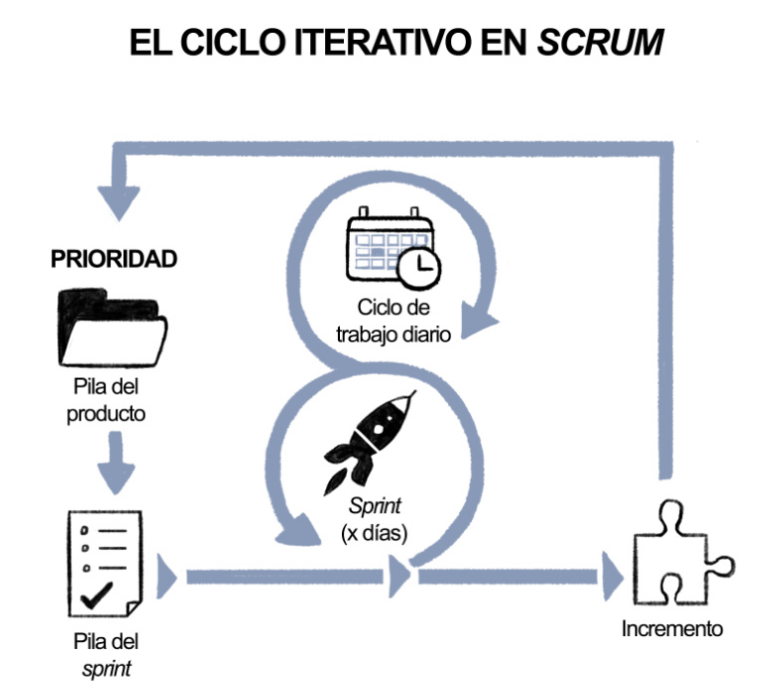
\includegraphics[scale=0.45]{../img/anexos/scrum/ciclo}
\end{figure}

\subsection{Roles}
Descripción de los posibles interventores durante el desarrollo de un producto.

\begin{itemize}
	\item \textit{Product owner}: es el representante del cliente, y su responsabilidad es el valor del producto. Es quien gestiona la pila del producto (conjunto de historias de usuario solicitadas por el cliente), así como la prioridad de cada ítem que lo compone.
	
	\item \textit{Scrum Master:} es el responsable de garantizar que el proyecto se desarrolla siguiendo los principios de \textit{scrum}, asesorando a los desarrolladores. También es el moderador en las reuniones diarias de \textit{scrum} y el encargado de resolver dinámicas que puedan perjudicar al equipo.
	
	\item \textit{Equipo de desarrollo:} es el conjunto de programadores autogestionados encargados de generar los incrementos. Profesionales multifuncionales, deben completar las tareas que se les asignen en el plazo estimado, además de participar en la toma de decisiones.
\end{itemize}

\subsection{Artefactos}

Son las <<herramientas>>~\cite{scrumMaster2022} elementales. Entre ellos se encuentran:

\begin{itemize}
	\item Pila de producto o \textit{product backlog}: contiene las historias de usuario (el equivalente a los <<requisitos>> en las metodologías tradicionales). Evoluciona durante el proyecto en función de las peticiones del cliente.
	\item Pila del \textit{sprint} o \textit{sprint backlog}: es la lista de tareas que han de completar los desarrolladores en un \textit{sprint}. En este proyecto, se han utilizado las \textit{milestones} de GitHub (asignándoles \textit{issues}) para representarla.
	\item Incremento: resultado de cada \textit{sprint}. Ha de ser un entregable.
	\item Gráfico de avance o \textit{burn down report}: muestra el trabajo pendiente por realizar en un \textit{sprint} y es actualizado por los desarrolladores. Indica, además, el ritmo de trabajo <<ideal>> que se debería seguir para alcanzar los objetivos. En este caso, se ha utilizado el gráfico generado por ZenHub.
	\item Gráfico de producto o \textit{burn up report}: mide cuánto se ha completado respecto al total.
\end{itemize}

\subsection{Eventos}
Durante el ciclo de \textit{scrum}, se pueden identificar varias actividades que constituyen la rutina y se represetan en la imagen~\ref{img:eventos_scrum} facilitada por el Manual de \textit{scrum}~\cite{scrumMaster2022}.

\begin{figure}[h]
	\caption{Eventos de \textit{scrum} según el Manual de \textit{scrum}~\cite{scrumMaster2022}.}
	\label{img:eventos_scrum}
	\centering
	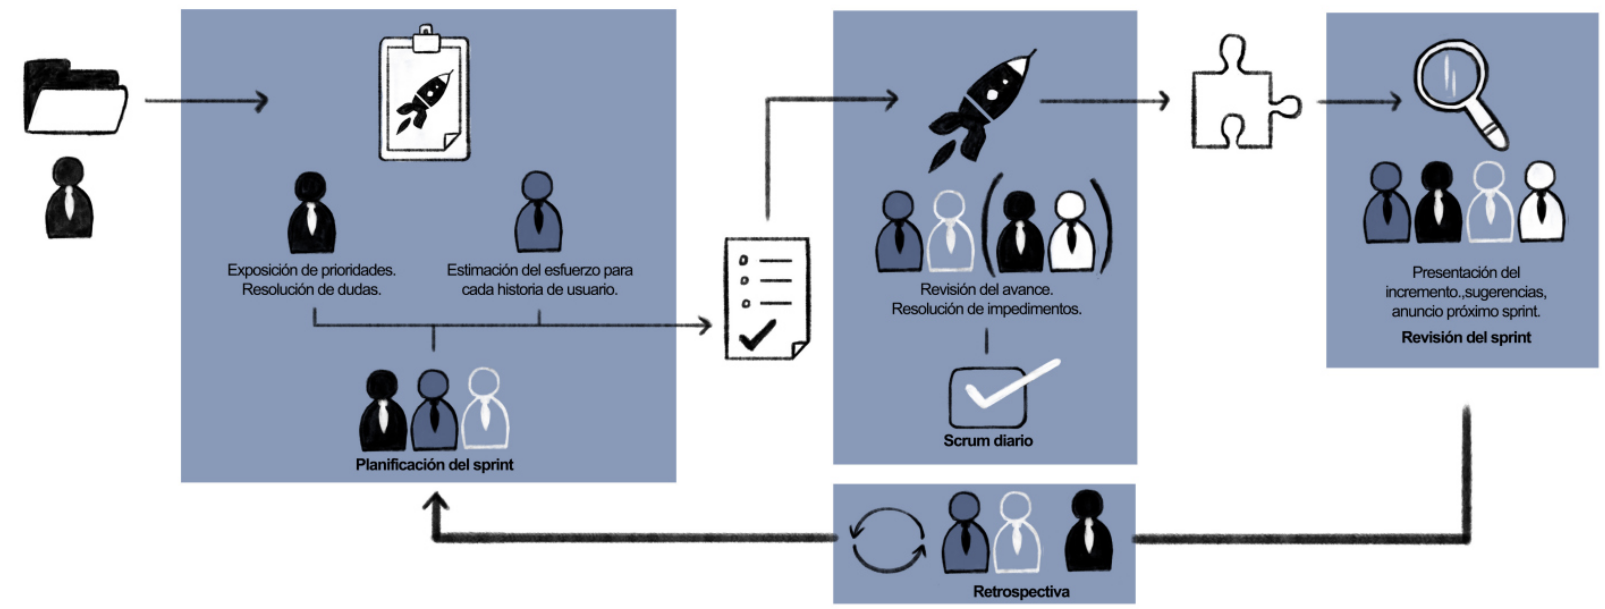
\includegraphics[width=\textwidth]{../img/anexos/scrum/eventos}
\end{figure}

\begin{enumerate}
	\item \textit{Sprint} o iteración: es un periodo de tiempo fijo (y breve) en el que se trabaja para completar una cantidad de tareas prefijadas con antelación (la pila del \textit{sprint}). Se han utilizado los \textit{sprints} de ZenHub para realizar el seguimiento.
	\item Reunión de planificación sel \textit{sprint}: marca el inicio de cada \textit{sprint} y determina las tareas a desarrollar, además de su duración temporal.
	\item\textit{Scrum} diario: breve reunión en la que cada integrante del equipo notifica su ritmo de trabajo con el fin de corregir posibles impedimentos que ralenticen el ciclo. Además, se actualiza el \textit{burndown report}. En este caso, debido a que el equipo está formado únicamente por un desarrollador, se ha omitido.
	\item Revisión del \textit{sprint}: se analiza el incremento entregado y se adapta la pila del producto en caso de necesitarlo (por ejemplo, si se ha encontrado algún \textit{bug} o se necesita refactorizar).
	\item Retrospectiva del \textit{sprint}: se aporta el \textit{feedback} necesario para mejorar la siguiente iteración.
\end{enumerate}

\subsection{Medición}

Como se puede observar, cada equipo puede realizar una cantidad de trabajo, generalmente fija, en cada \textit{sprint}. Por ello, es necesario estimar el tiempo que requiere cada tarea y no asignar más trabajo del que se pueda asimilar en cada iteración.

En este proyecto, se han utilizado los <<puntos de historia>> como unidad de medida.


\section{Planificación temporal}

\subsection{Planificación por \textit{sprints}}

Siguiendo los eventos de \textit{scrum}, y adaptándolos teniendo en cuenta el tamaño del equipo (un desarrollador), se ha decidido planificar el proyecto mediante \textit{sprints}.

\subsubsection{\textit{Sprint 1: Mustard}}

\begin{itemize}
	\item \textbf{\textit{Planning meeting}}
	
	Durante la reunión se marcaron los siguientes objetivos:
	
	\begin{enumerate}
		\item Configuración básica: incluyendo la creación del repositorio, la correcta instalación de ZenHub, la creación de entornos virtuales (miniconda, SKLearn, etc.) y la familiarización con conceptos \textit{scrum}: \textit{milestones, sprints, epics}, etc.
		\item Memoria: comienzo de la redacción incluyendo las secciones de introducción, conceptos teóricos (aprendizaje automático) y trabajo relacionado.
		\item Investigación: búsqueda del código SSADR-CoF y de las bases de datos utilizadas en el paper.
		\item Lectura de papers: Engelen \& Hoos~\cite{engelen2020surveyOnSemiSupervised}, García, Triguero \& Herrera~\cite{triguero2015SelflabeledTechniques}, y Zhou \& Duan~\cite{zhou2021SemisupervisedRecommendationAttack}.
	\end{enumerate}
	
	\item \textbf{Marcas temporales}
	El \textit{sprint} se desarrolló entre el 24 de septiembre de 2022 y el 2 de octubre del 2022.
	
	\item \textbf{\textit{Burndown Report}}
	\begin{figure}[h]
		\caption{\textit{Burndown Report Sprint 01}}
		\centering
		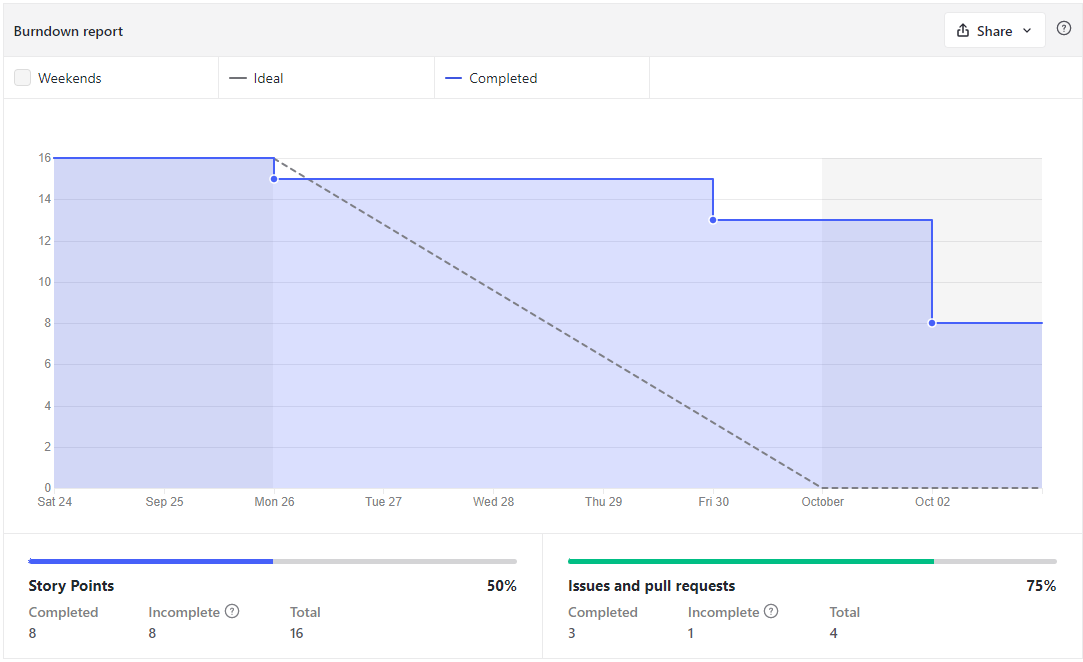
\includegraphics[width=\textwidth]{../img/anexos/bdr/s01_bdr}
	\end{figure}
	
	Como se puede comprobar, no todos los objetivos marcados fueron cumplidos: la estimación del tiempo fue demasiado optimista, además de no contar con el tiempo requerido en solucionar problemas técnicos (\LaTeX{}). Se dejó para próximos sprints la lectura del último paper.

	\item \textbf{\textit{Sprint review meeting}}
	Durante la reunión se fijaron ciertas correcciones en la memoria (mejorar referencias bibliográficas y la sección de <<Trabajos relacionados>>), además de la necesidad de introducir una sección teórica de ataques a los sistemas de recomendación.
	
\end{itemize}


\subsubsection{\textit{Sprint 2: Paprika}}
\begin{itemize}
	\item \textbf{\textit{Planning meeting}}
	Objetivos del siguiente Sprint:
	
	\begin{enumerate}
		\item Configuración: debido a la gran cantidad de tiempo invertida en solucionar errores de compilación en \LaTeX{}, se decidió migrar el proyecto a una nueva instalación basada en Debian.
		\item Correcciones: aspectos estilísticos y completar información.
		\item Lectura: Mingdan y Qingshan~\cite{mingdan2018ShillingAttacksAReview} con el objetivo de introducir una sección teórica de ataques.
		\item Memoria: redacción completa de los modelos de ataque en los aspectos teóricos.
		
	\end{enumerate}
	
	\item \textbf{Marcas temporales}
	El \textit{sprint} se desarrolló entre el 3 de octubre de 2022 y el 18 de octubre del 2022.
	
	\item \textbf{\textit{Burndown Report}}
	\begin{figure}[h]
		\caption{\textit{Burndown Report Sprint 02}}
		\centering
		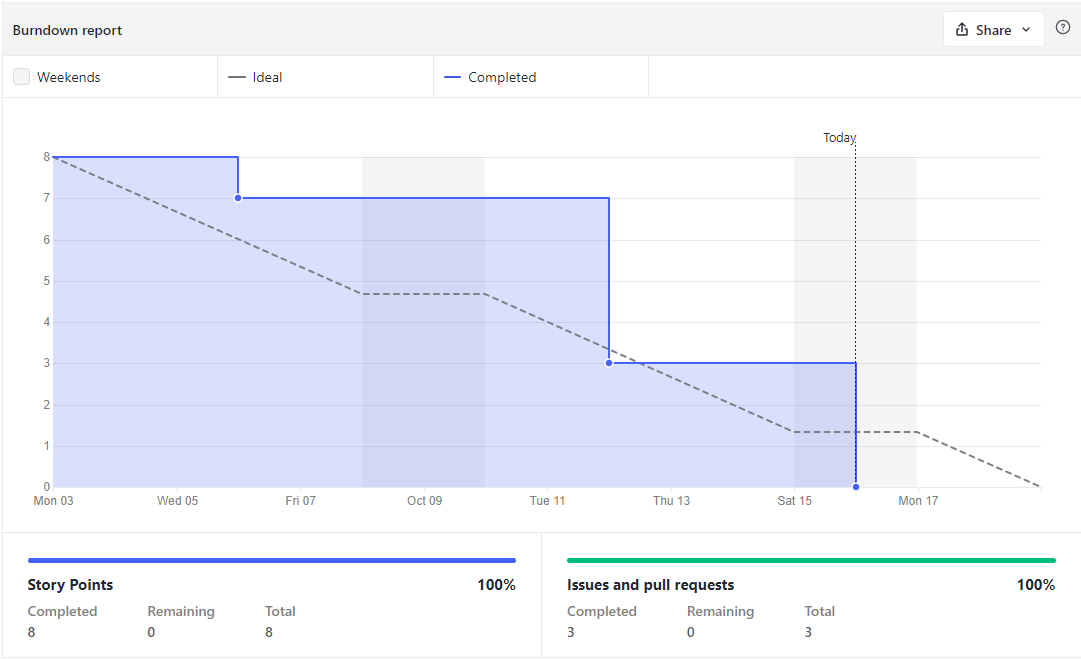
\includegraphics[width=\textwidth]{../img/anexos/bdr/s02_bdr}
	\end{figure}
		
	En este \textit{sprint} sí se cumplió con los objetivos marcados. Sin embargo, la estimación de tiempo tampoco fue la adecuada, requiriendo más de lo previsto.
	\item \textbf{\textit{Sprint review meeting}}
	Durante la reunión se resolvieron dudas acerca de bibliografía, referencias y trabajo previo. Además, se acordó empezar a programar, definiendo así los \textit{issues} desarrollados en el siguiente \textit{sprint}.
	
\end{itemize}

\subsubsection{\textit{Sprint 3: Fennel Seeds}}
\begin{itemize}
	\item \textbf{\textit{Planning meeting}}
	
	Durante esta reunión, se decidió empezar a programar el \textit{co-forest}. Para ello, se definieron los siguientes pasos:
	
	\begin{enumerate}
		
		\item Librerías: se acordó aprender a utilizar las librerías más comunes en el \textit{data science}. Entre ellas: MatplotLib y SKLearn. Además, se requirió la correcta configuración del entorno virtual, haciendo que el tiempo dedicado al \textit{issue} fuese mayor de lo estimado (problemas en el \texttt{PATH} y con las dependencias).
		
		\item \textit{SKLearn}: aprovechando la correcta documentación de la librería, se decidió repasar los conceptos teóricos básicos, además del manejo de la <<interfaz>> (métodos comunes). Entre ellos:
		
		\begin{itemize}
			\item \textit{Decision trees}
			\item \textit{Self training}
			\item \textit{Random Forest}
		\end{itemize}
	
		\item Lectura: se concertó la relectura del artículo de Zhou~\cite{zhou2021SemisupervisedRecommendationAttack} con la intención de comprender el algoritmo y del \textit{paper} <<original>> del \textit{co-forest}~\cite{originalCoForest2007}. Durante el proceso de programación, además, se encontró la tesis de Van Engelen~\cite{engelen2018thesis} y se añadió al conjunto.
		\item Documentación: se acordó la corrección de los errores previamente señalados y la inclusión del \textit{sprint} en los anexos.
		\item Programación del \textit{Co-Forest}: se programó el pseudocódigo ilustrado en la Tesis de Van Engelen~\cite{engelen2018thesis}, que es muy similar al original~\cite{originalCoForest2007} pero con algunas diferencias. Inicialmente se intentó usar el \textit{Random Forest} de \textit{SKLearn}, pero se descartó la idea debido a la poca versatilidad que se ofrecía para manejar los \textit{concomitant ensembles}. Se han de corregir ciertos factores, pero se pospondrá hasta la correcta discusión con el tutor.
		
	\end{enumerate}
	
	\item \textbf{Marcas temporales}	
	El \textit{sprint} se desarrolló entre el 19 de octubre de 2022 y el 2 de noviembre del 2022.
	
	\item \textbf{\textit{Burndown Report}}
	
		\begin{figure}[h]
		\caption{\textit{Burndown Report Sprint 03}}
		\centering
		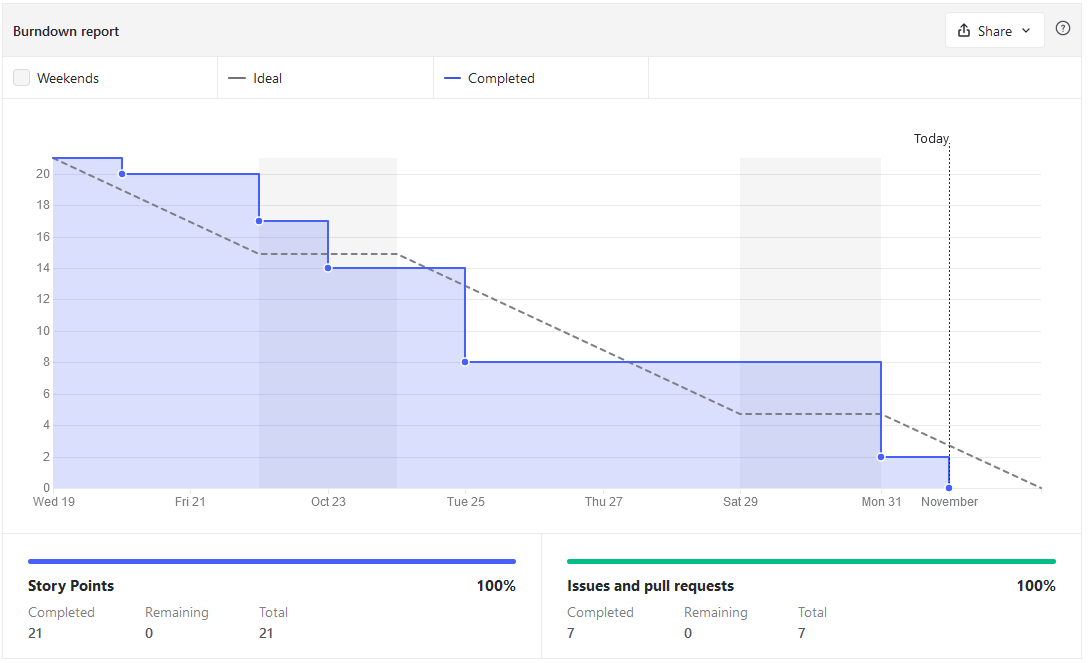
\includegraphics[width=\textwidth]{../img/anexos/bdr/s03_bdr}
		\end{figure}
	
	En este \textit{sprint} se cumplió con los objetivos marcados. Nuevamente, la estimación del tiempo fue inferior a la real (se pensaba que se podría depender más de librerías existentes de lo que se pudo en realidad), calculándose un total de aproximadamente 25 horas reales.

	\item \textbf{\textit{Sprint review meeting}}
	
	Durante la revisión del \textit{sprint}, se llegó a la conclusión de que el pseudocódigo podía ser mejor implementado aprovechando ciertas librerías de \textit{Python}. Se comentó cómo mejorar complejidades espaciales y reducir el código. Se fijaron objetivos para las próximas semanas.
	
\end{itemize}


\subsubsection{\textit{Sprint 4: Cayenne}}
\begin{itemize}
	\item \textbf{\textit{Planning meeting}}
	
	Durante la reunión se acordaron los siguientes objetivos:
	
	\begin{enumerate}
		\item Reimplementación del código: se acordó volver a programar el \textit{co-forest}, esta vez implementando una versión más <<\textit{pythoniana}>> con el fin de mejorar la complejidad espacial y facilitar la lectura.
		\item Curso de Numpy: se decidió que sería interesante la realización de un curso para aprender a utilizar la librería y aplicarla al código.
		\item Curso de Pandas: aprovechando la relación con el punto anterior, se acordó completar también un curso de esta librería.
		\item Memoria: corregir aspectos anteriores e incluir toda la teoría relacionada con el \textit{co-forest}.
	\end{enumerate}
	
	\item \textbf{Marcas temporales}
	El \textit{sprint} se desarrolló entre el 3 de noviembre de 2022 y el 15 de noviembre del 2022.
			
	\item \textbf{\textit{Burndown Report}}
	\begin{figure}[h]
		\caption{\textit{Burndown Report Sprint 04}}
		\centering
		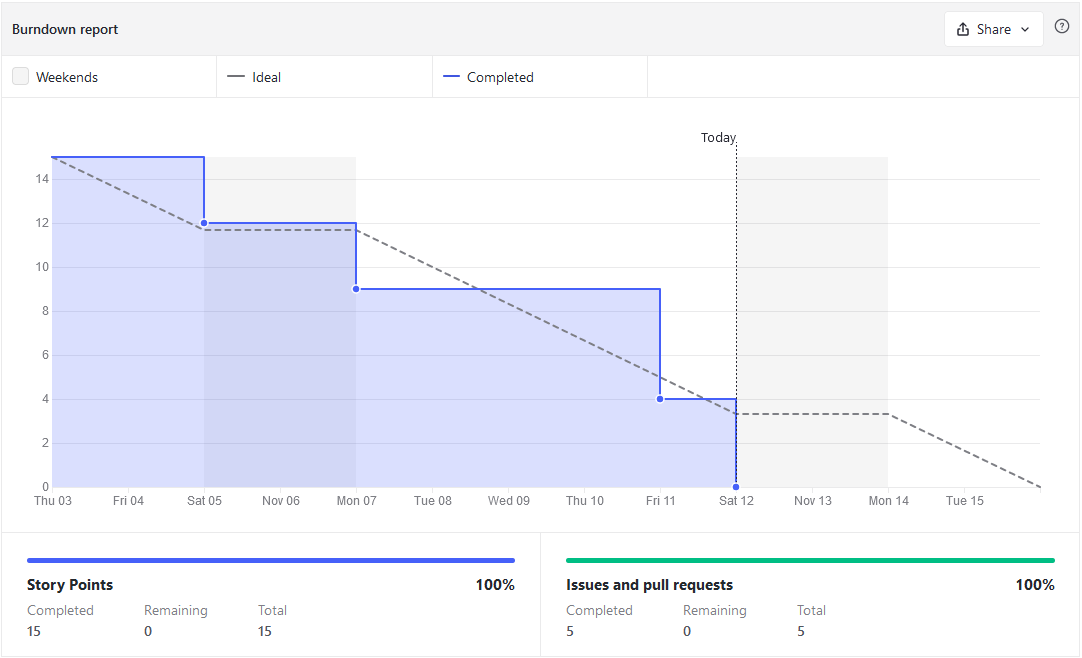
\includegraphics[width=\textwidth]{../img/anexos/bdr/s04_bdr}
	\end{figure}
	
	En este \textit{sprint} se completaron los objetivos, aunque quedaron pendientes ciertos aspectos a comentar respecto al código. Destacar que, debido a que se terminaron antes de lo planeado los \textit{issues} planificados, se aprovechó para modificar ciertos aspectos pendientes relacionados con la memoria y para probar correctamente el código. Esto hizo que el tiempo real dedicado haya sido ligeramente superior al estimado (más tiempo de documentación).
	
	\item \textbf{\textit{Sprint review meeting}}
	En la reunión se acordó experimentar con el algoritmo utilizando distintos conjuntos de datos, además de mejorar ciertos detalles de implementación.
	
\end{itemize}

\subsubsection{\textit{Sprint 5: Curry}}

\begin{itemize}
	\item \textbf{\textit{Planning meeting}}
		Durante la reunión se acordaron los siguientes objetivos:
	
	\begin{enumerate}
		\item Ajustes al código: se acordó mejorar algunos factores, como la generación de objetos <<aleatorios>> para obtener resultados deterministas en los experimentos, optimización de memoria o corrección de parámetros.
		\item Experimentación: se determinó probar el código con distintos conjuntos de datos en diferentes fases: durante el entrenamiento y tras terminarlo. Para ello, se estudiaron algunos conceptos teóricos y el uso de la librería MatplotLib para representar gráficamente los resultados obtenidos.
		\item Memoria: documentación de los experimentos realizados y correcciones.
	\end{enumerate}

	\item \textbf{Marcas temporales}		
	El \textit{sprint} se desarrolló entre el 15 de noviembre de 2022 y el 25 de noviembre del 2022.
	
	\item \textbf{\textit{Burndown Report}}
		\begin{figure}[h]
		\caption{\textit{Burndown Report Sprint 05}}
		\centering
		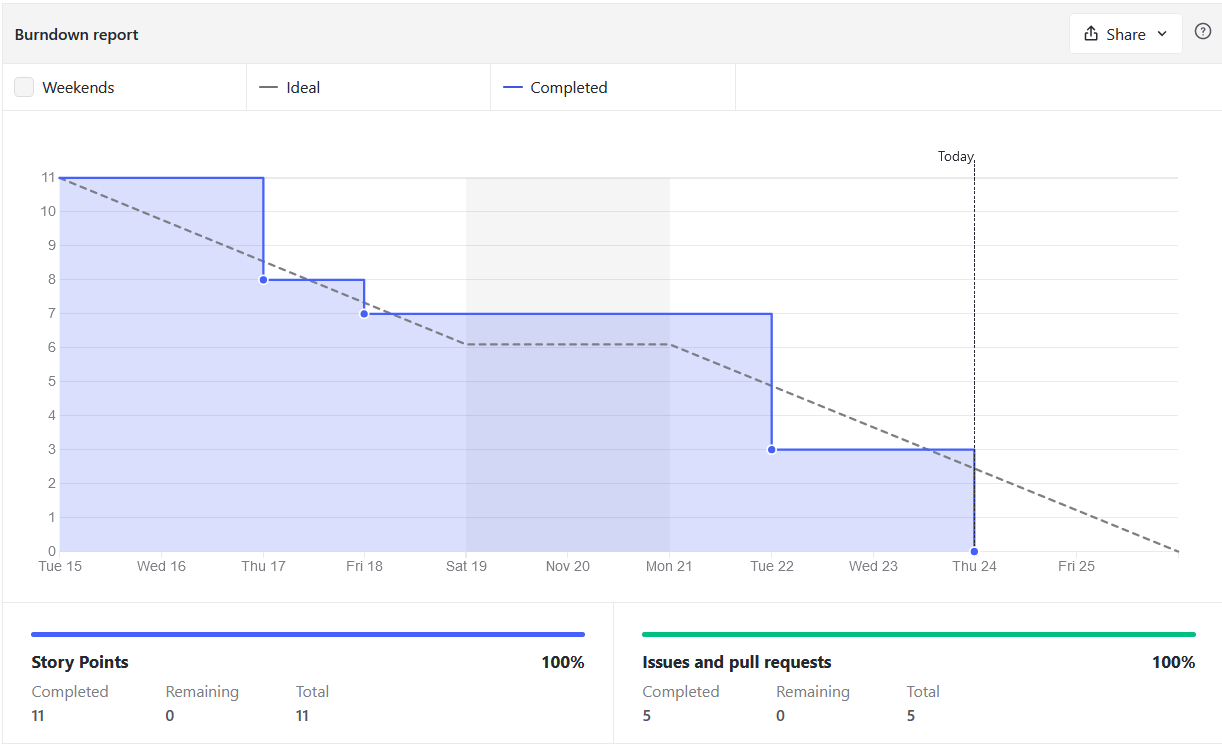
\includegraphics[width=\textwidth]{../img/anexos/bdr/s05_bdr}
	\end{figure}
	
	En este \textit{sprint} se cerraron todos los puntos de historia propuestos. Aunque se estimaron 11 horas de trabajo, el tiempo invertido fue superior, realizando 15. La mayor dedicación se justifica por la existencia de reuniones intermedias y de <<defectos>> encontrados en el código en el trascurso del \textit{sprint}.
	
	\item \textbf{\textit{Sprint review meeting}}
	Durante la reunión se acordó comparar los resultados obtenidos con los de otras herramientas, además de empezar el tratamiento de los conjuntos de datos utilizados en el \textit{paper}~\cite{zhou2021SemisupervisedRecommendationAttack}.
	
\end{itemize}


\subsubsection{\textit{Sprint 6: Coriander}}
\begin{itemize}
	\item \textbf{\textit{Planning meeting}}
	Durante la reunión se fijaron los siguientes objetivos:
	
		\begin{enumerate}
		\item Ajustes en las gráficas: arreglar detalles menores en el formato de ciertos gráficos.
		\item Comparativas: probar los resultados obtenidos y compararlos la herramienta de la Universidad de Granada llamada \textit{Keel}.
		\item \textit{Datasets} <<reales>>: probar el algoritmo utilizando MovieLens, una de las bases de datos utilizadas en el \textit{paper}~\cite{zhou2021SemisupervisedRecommendationAttack}. Para ello, es necesaria una re-lectura del artículo y realizar el procesamiento inicial de los datos.
		\item Memoria: documentación de los experimentos realizados.
	\end{enumerate}

	\item \textbf{Marcas temporales}		
	El \textit{sprint} se desarrolló entre el 25 de noviembre de 2022 y el 5 de diciembre del 2022.
	
	\item \textbf{\textit{Burndown Report}}
		\begin{figure}[h]
			\caption{\textit{Burndown Report Sprint 06}}
			\centering
			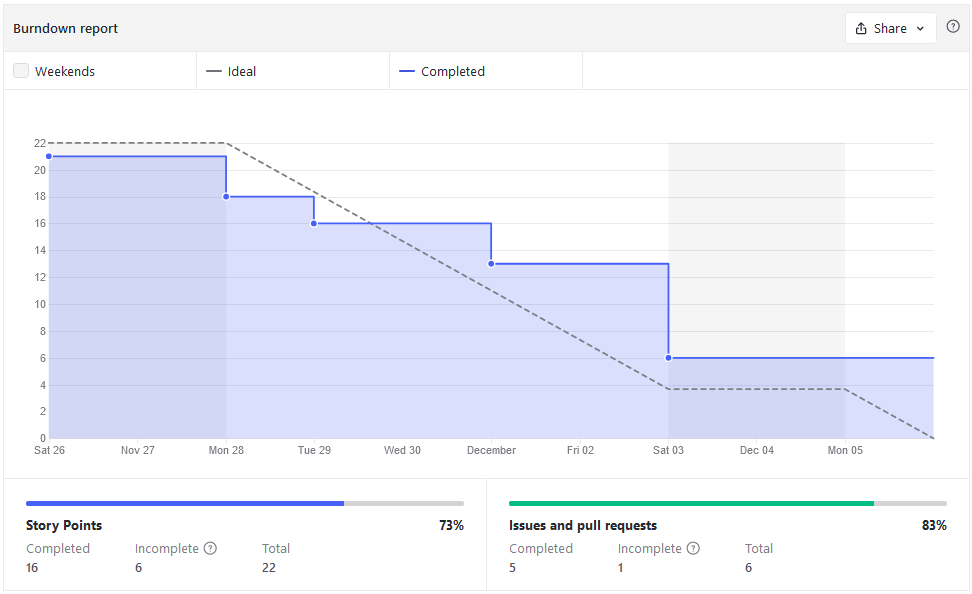
\includegraphics[width=\textwidth]{../img/anexos/bdr/s06_bdr}
		\end{figure}
	
	Puede parecer que los puntos de historia fueron mal estimados debido a que el ritmo de trabajo es bajo. Sin embargo, se justifica debido a que durante la experimentación (en concreto, durante la comparativa contra KEEL) se encontraron dos \textit{bugs} en el código (causados no por la lógica del programa, sino por el operador \textit{in} de Python y por no estar preparado para recibir etiquetas que no comiencen en 0).
	
	Debido a que los errores se encontraron una vez se realizó toda la documentación, se tuvo que repetir la sección asociada a los experimentos del \textit{co-forest}, además de localizar y depurar los errores de código. Todo este trabajo supuso un esfuerzo extra de 7 horas, que fueron introducidas en el \textit{backlog} del \textit{sprint} a mediados del mismo (debido a la gran importancia que tienen y la influencia en pasos posteriores). Por este motivo, no se completaron los objetivos previstos. Sin embargo, el tiempo dedicado al proyecto fue el estimado.
	
	Es destacable también que de los 6 puntos de historia que quedan se realizaron 2, pero se decidió dejar el \textit{issue} abierto para el siguiente \textit{sprint}.

	\item \textbf{\textit{Sprint review meeting}}
	
	Habiendo finalizado el modelo, se decidió empezar a experimentar con bases de datos de sistemas de recomendación. Además, se acordó añadir nuevas gráficas.
\end{itemize}

\subsubsection{\textit{Sprint 7: Cinnamon }}
\begin{itemize}
	\item \textbf{\textit{Planning meeting}}
	
	Se marcaron los siguientes objetivos para el \textit{sprint}.
	
	\begin{enumerate}
		\item Extraer vectores de características: estudiar e implementar el método de extracción de vectores por ventanas expuesto en el \textit{paper} de Zhou y Duan~\cite{zhou2021SemisupervisedRecommendationAttack}. Generar ficheros \texttt{.csv} con dichos vectores para poder importarlos posteriormente con Pandas. Probar la correcta generación de vectores con perfiles verdaderos y atacantes.
		\item Generación de reseñas de atacantes: siguiendo los modelos estadísticos, generar reseñas de ataque para el \textit{random attack}, el \textit{average attack} y el \textit{bandwagon attack}.
		\item Documentación: añadir introducción y descripción de \textit{scrum} en los anexos. Corregir las sugerencias anteriores. Incluir la descripción del método de extracción de vectores de características por ventanas y la generación de reseñas de atacantes.
	\end{enumerate}
	
	\item \textbf{Marcas temporales}		
	El \textit{sprint} se planificó para desarrollarse entre el 8 y el 20 de diciembre de 2022. Sin embargo y debido al ritmo de trabajo, se cerró el 15 de diciembre de 2022.
	
	\item \textbf{\textit{Burndown Report}}
	\begin{figure}[h]
		\caption{\textit{Burndown Report Sprint 07}}
		\centering
		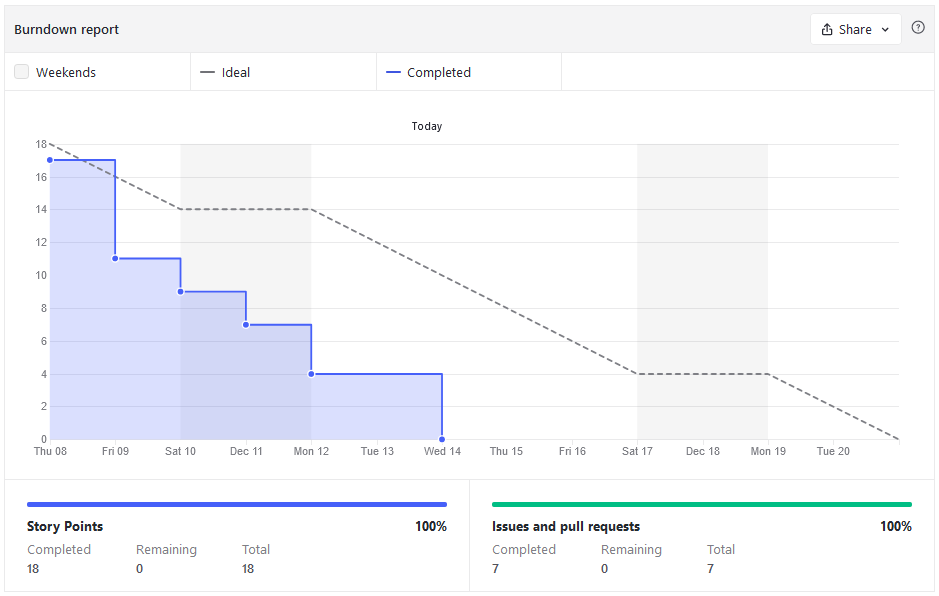
\includegraphics[width=\textwidth]{../img/anexos/bdr/s07_bdr}
	\end{figure}

	Como se puede comprobar, se finalizaron las tareas del \textit{sprint} antes de lo previsto. En gran parte, debido a que el \textit{issue} de extracción de vectores de características estaba ya comenzado en el \textit{sprint} anterior, y requirió menos tiempo del planificado. Además, el resto de tareas no dieron problemas en esta iteración. Debido a que \textit{scrum} no permite añadir nuevos ítems en la pila del \textit{sprint} durante el desarrollo de este, se decidió cerrar y comenzar uno nuevo.

	\item \textbf{\textit{Sprint review meeting}}
	
	Durante la reunión se concluyó que la forma de generar vectores de características y reseñas de ataques es correcta, por lo que se decidió experimentar con el \textit{co-forest} y datos reales.
	
\end{itemize}



\subsubsection{\textit{Sprint 8: Kaffir Lime Leaves}}
\begin{itemize}
	\item \textbf{\textit{Planning meeting}}
	
	Durante este \textit{sprint} se fijaron los siguientes objetivos:
			\begin{enumerate}
			\item Refactorizar el extractor de vectores de características y el generador de reseñas de atacantes: debido a que la sintetización de los conjuntos de entrenamiento y \textit{test} requiere demasiado tiempo ($25h$), se ha decidido mejorar la complejidad algorítmica y convertir a clase con el fin de reducir llamadas con mayor complejidad temporal.
			\item Completar el \textit{co-forest}: añadir nuevos métodos para realizar comparaciones (predicción con probabilidades, AUC, \textit{recall} y precisión).
			\item Orden de repositorio: lectura acerca de la creación de módulos en python, conversión de los \textit{notebooks} a archivos \texttt{.py} importables, configuración de rutas.
			\item Análisis de resultados: analizar los resultados en busca de posibles errores cometidos durante la experimentación.
			\item Generación de gráficas y comparación contra \textit{random forest}: utilizando clases de SKLearn, automatizar la generación de gráficas para imitar el experimento realizado por Zhou y Duan~\cite{zhou2021SemisupervisedRecommendationAttack} para el \textit{co-forest} y dos \textit{random forest} con distintos conjuntos de entrenamiento.
			\end{enumerate}
		
	\item \textbf{Marcas temporales}	
	
	Para evitar solapamientos con el \textit{sprint} anterior, oficialmente (en el repositorio) se desarrolló entre el 18 y el 22 de Diciembre del 2022. Sin embargo, se empezó unos días antes.	
	
	\item \textbf{\textit{Burndown Report}}
	
	\begin{figure}[h]
		\caption{\textit{Burndown Report Sprint 08}}
		\centering
		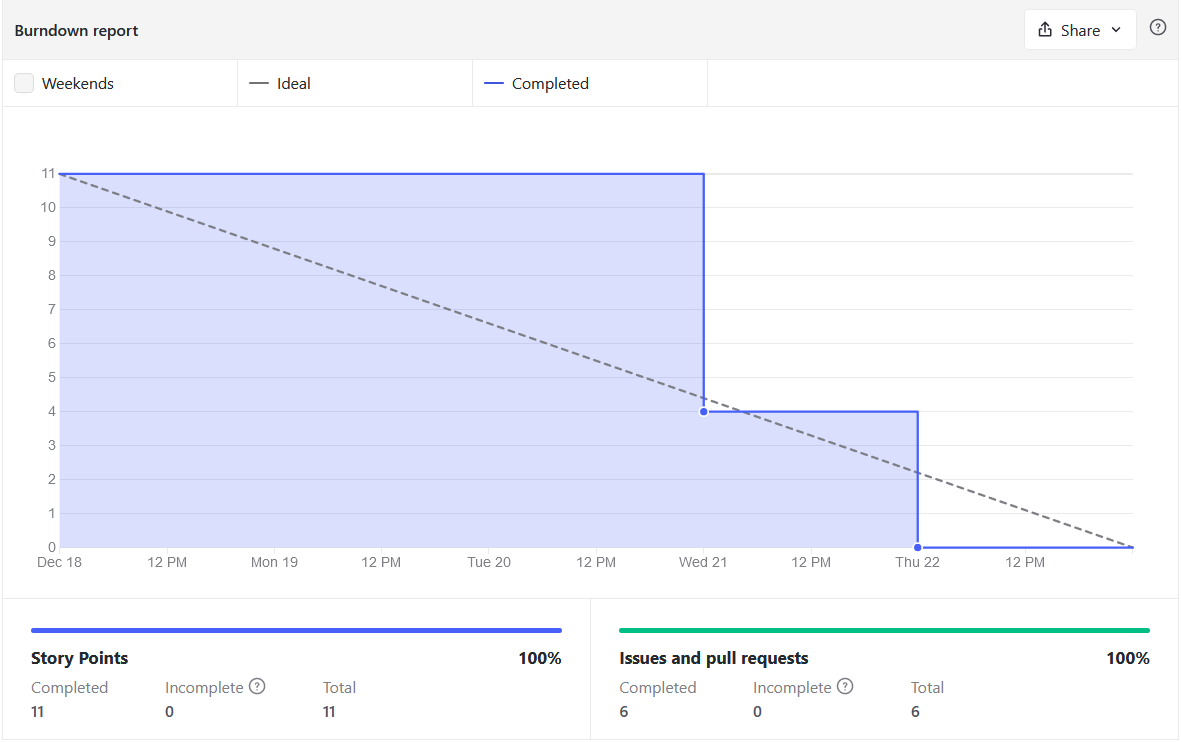
\includegraphics[width=\textwidth]{../img/anexos/bdr/s08_bdr}
	\end{figure}

	Como se puede comprobar, los \textit{issues} fueron completados correctamente.	

	\item \textbf{\textit{Sprint review meeting}}
	Durante la reunión se comprobó que los resultados obtenidos en la fase de experimentación no se asemejan a los presentados en el \textit{paper} seguido~\cite{zhou2021SemisupervisedRecommendationAttack}. Sin embargo, se concluyó que deberían ser correctos. Para evitar realizar afirmaciones erróneas, se decidió revisar todo el proceso de experimentación.
\end{itemize}



\subsubsection{\textit{Sprint 9: Ginger}}
\begin{itemize}
	\item \textbf{\textit{Planning meeting}}
	
	Debido a que este \textit{sprint} se realizó durante la época vacacional, se decidió realizar una revisión general del documento completando aspectos pendientes.
	
	\begin{enumerate}
		\item Experimentación \textit{co-forest}: se incluyó una gráfica \textit{extra} pendiente (tiempo de entrenamiento-número de árboles) y se repitió la experimentación esta vez utilizando conjuntos estratificados. Se corrigieron los cambios surgidos y actualizaron las gráficas en la memoria. Se revisó la clase del \textit{co-forest} y se terminó de documentar.
		\item Documentación: se decidió cerrar aspectos pendientes. Entre ellos: completar las secciones teóricas de semisupervisado, ensembles y métricas, repetir gráficas e ilustraciones incorrectas, revisar la bibliografía y trabajos relacionados, completar los anexos y corregir aspectos menores.
		\item Revisión de la detección de ataques: debido a que los resultados obtenidos no son los esperados, se decidió revisar toda la generación de reseñas de atacantes, extracción de perfiles y métodos de experimentación en busca de posibles errores.
		\item Implementación: comenzar a implementar el \textit{democratic-co} y leer sobre él.
	\end{enumerate}

	\item \textbf{Marcas temporales}		
	El \textit{sprint} se desarrolló entre el 27 de Diciembre del 2022 y el 8 de Enero del 2023.
	
	
	\item \textbf{\textit{Burndown Report}}
	...
	
	El número total de horas dedicadas al proyecto fue de 20. Como algunos de los \textit{issues} requirieron menos tiempo del planificado (en especial los relacionados con la documentación), se destinó el tiempo sobrante a otros pendientes.
	
	
	\item \textbf{\textit{Sprint review meeting}}
\end{itemize}







\subsubsection{\textit{Sprint N: }}
\begin{itemize}
	\item \textbf{\textit{Planning meeting}}
	\begin{enumerate}
		\item
		\item
		\item
		\item 
	\end{enumerate}
	\item \textbf{Marcas temporales}		
	\item \textbf{\textit{Burndown Report}}
	\item \textbf{\textit{Sprint review meeting}}
\end{itemize}
\section{Estudio de viabilidad}

\subsection{Viabilidad económica}

\subsection{Viabilidad legal}



\apendice{Especificación de Requisitos}

\section{Introducción}

La fase de análisis es una etapa fundamental en el ciclo de vida del desarrollo ya que permite entender los requerimientos del cliente e identificar los componentes necesarios para entregar un producto adecuado.

Durante esta fase, el equipo de desarrollo se reune con el cliente (o con su representante el \textit{product owner}) y, tras realizar diversas entrevistas, se recoge lo que este espera de la aplicación. Además, el equipo de desarrollo analizará todos los requisitos no relacionados con la funcionalidad (como puede ser seguridad, escalabilidad, rendimiento, etc.) que se puedan deducir de dichas conversaciones.

Debido a la importancia que tiene esta fase, se ha experimentado una evolución con los años y se han propuesto distintas aproximaciones en función de las metodologías utilizadas. Entre ellas:

\begin{itemize}
	\item \textbf{Metodologías tradicionales}: estas metodologías realizan la captura de los requerimientos en fases tempranas del desarrollo, realizando una <<fotografía>> exacta (e, idealmente, inmutable) de lo que el usuario necesita. Para ello, se hace uso de requisitos funcionales y no funcionales que se documentan en un formato estructurado y definido en estándares. Un ejemplo de especificación es el estándar IEEE 830~\cite{ieee830}, donde se implora que los requisitos han de ser claros, precisos, medibles, coherentes, completos, factibles, específicos y verificables.
	
	\item  \textbf{Metodologías ágiles}: en contraposición, las metodologías ágiles tratan de ser flexibles y adaptarse al usuario (ya que, muchas veces, es común que no tenga claro en etapas tempranas de desarrollo lo que realmente necesita). Para ello utilizan las denominadas historias de usuario, que son breves descripciones de las funcionalidades que el usuario necesita para realizar una tarea específica. Estos documentos se recogen en estructuras tabulares y se almacenan en el \textit{product backlog}, que lejos de ser una <<fotografía>>, es una lista <<viva>> que se actualiza y prioriza en función de las necesidades del cliente. 
\end{itemize}


Aunque en un proyecto real puede no resultar óptimo realizar una <<mezcla>> de metodologías, debido a las peculiares características de este (equipo de un desarrollador) y a que se solicita la inclusión de requisitos funcionales y no funcionales de una manera más tradicional en la memoria, se ha hecho uso de ambos métodos de documentación (complementados, además, mediante prototipos expuestos en la sección~\ref{s:mockups}). Por lo tanto, se realizará una especificación de requisitos clásica (expuesta en la sección~\ref{s:cat-requisitos} y desarrollada en la sección~\ref{s:requisitos}) complementada con alguna historia de usuario extraída de las entrevistas con el \textit{product owner} (sección~\ref{s:hu}).

Cabe destacar que durante el desarrollo real se ha utilizado una metodología ágil mediante el uso de \textit{sprints} como se ha expuesto en la sección~\ref{s:planificacion-sprints}.

\section{Objetivos generales}

En este proyecto se han definido distintos objetivos que pueden ser resumidos en los siguientes puntos:

\begin{enumerate}
	\item Implementación y validación de algoritmos de aprendizaje semisupervisado: en concreto el \textit{co-forest}, el \textit{democratic-co learning} y el \textit{tri-training}.
	\item Aplicación del \textit{machine learning} a la solución de un problema real relacionado con la ciberseguridad: se ha escogido la detección de \textit{phishing} y detección de ataques en sistemas de recomendación, aunque esta última ha sido descartada por su bajo desempeño.
	\item Desarrollo de una herramienta que permita poner al servicio de la comunidad el conocimiento desarrollado: se ha decidido desarrollar un analizador de \textit{phishing} en formato página \textit{web}, permitiendo además administración avanzada de modelos de \textit{machine learning} e instancias de aprendizaje (URLs legítimos y fraudulentos).
\end{enumerate}

Como se puede intuir, los dos primeros están enfocados a la investigación mientras que el último es una tarea de desarrollo. Por este motivo, este anexo se centrará principalmente en el tercer punto.

\section{Usuarios}
\label{s:usuarios}

En las metodologías ágiles no sólo es necesario definir las funcionalidades, sino también quién las realiza. Por ello, se introducen a continuación los distintos usuarios de la página \textit{web} desarrollada, aunque sus funciones completas se pueden observar en el diagrama de casos de uso~\ref{b:diagrama-cu}.

\section{Catálogo de historias de usuario}
\label{s:hu}

\begin{table}
	\scalebox{0.80}{
	\begin{tabular}{@{}p{3em} p{6em} p{9em} p{9em} p{9em}@{}}		
	\toprule
	\textbf{ID} & \textbf{Como} & \textbf{Quiero} & \textbf{Para} & \textbf{Aceptación}\\
	\midrule
		& & & & \\
	\bottomrule
	\end{tabular}
	}
	\caption[Historias de usuario:]{Ejemplo de estructura tabular para recoger una historia de usuario}
	\label{hu:estructura-tabular}
\end{table}


\section{Catálogo de requisitos}
\label{s:cat-requisitos}

\section{Prototipado}
\label{s:mockups}

Como es conocido, en el mundo del desarrollo \textit{software} suele haber una diferencia en el entendimiento de una aplicación por parte del cliente y del equipo de desarrollo que puede desembocar en malentendidos que causen retrasos temporales y pérdidas económicas.

Con el fin de reducir dichas desventajas y realizar un diseño que se adapte a los requerimientos del usuario, se ha decidido realizar una fase de prototipado durante las entrevistas del producto. Esto ha permitido identificar posibles diferencias entre el equipo del desarrollo y el cliente (representado por el \textit{product owner}), facilitando la comunicación y colaboración entre ambas partes.

Se adjuntan a continuación los diferentes \textit{mockups} del analizador de \textit{phishing} realizados durante esta fase.


\begin{figure}[h]
	\caption{Prototipos: página principal}
	\centering
	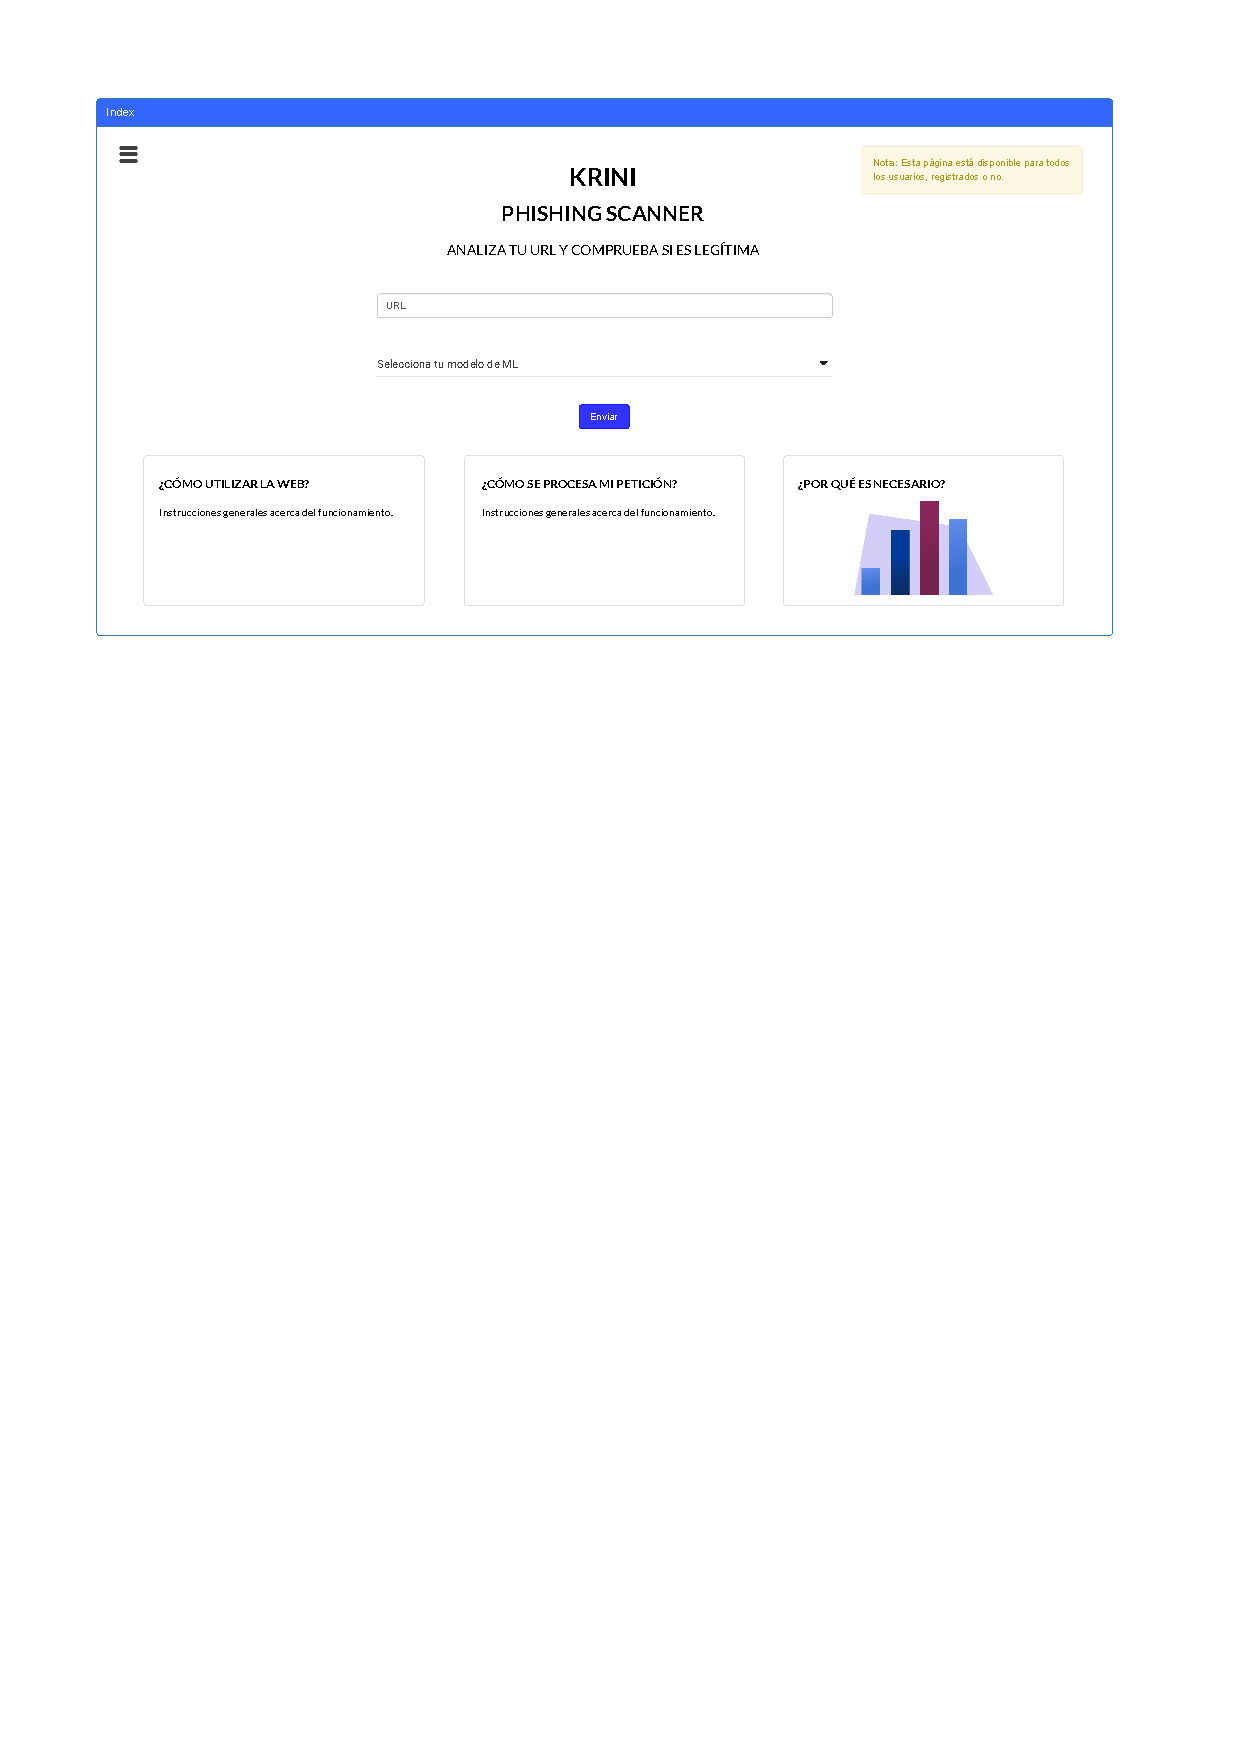
\includegraphics[width=\textwidth]{../img/anexos/mockups/1-mockups-index}
	\label{mock:index}
\end{figure}

\begin{figure}[h]
	\caption{Prototipos: \textit{dashboard}}
	\centering
	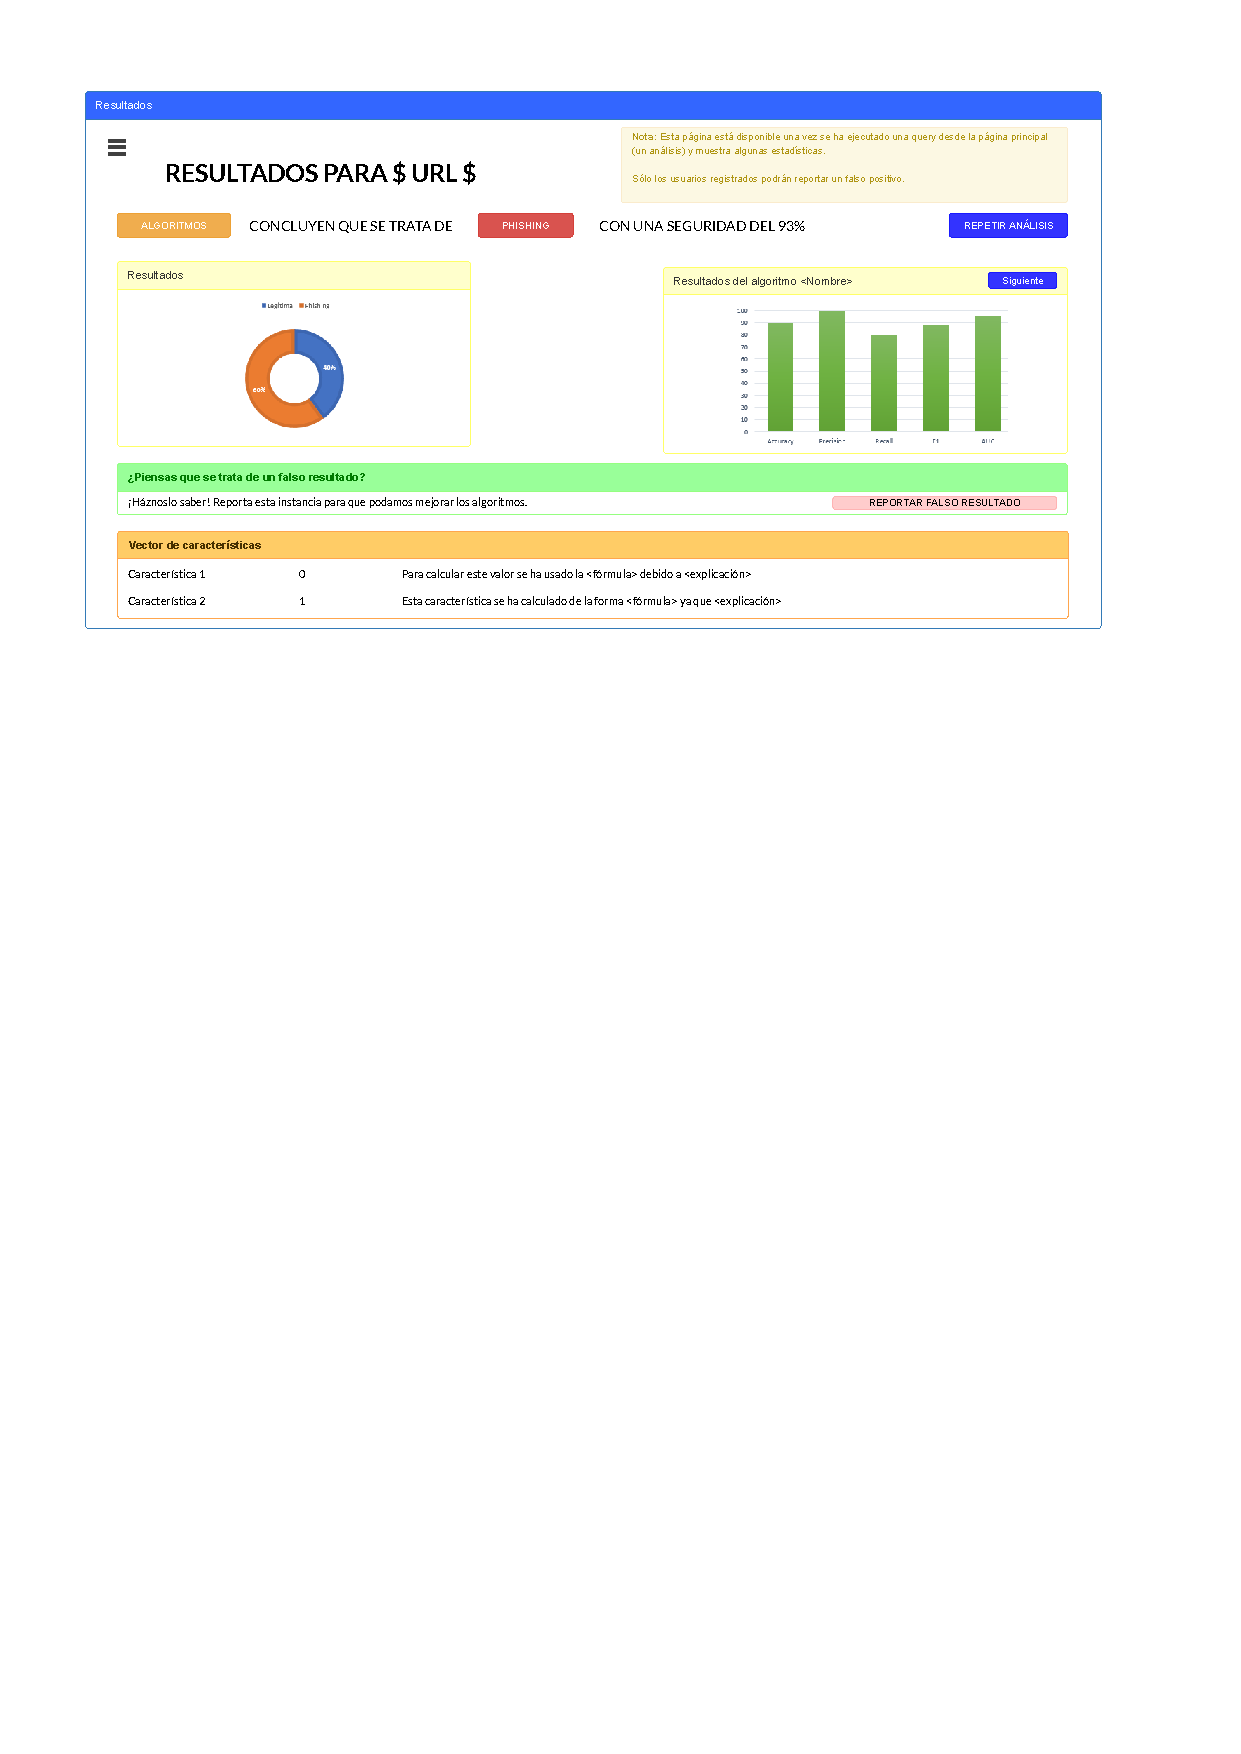
\includegraphics[width=\textwidth]{../img/anexos/mockups/2-mockups-dashboard}
	\label{mock:dashboard}
\end{figure}

\begin{figure}[h]
	\caption{Prototipos: reportar una URL}
	\centering
	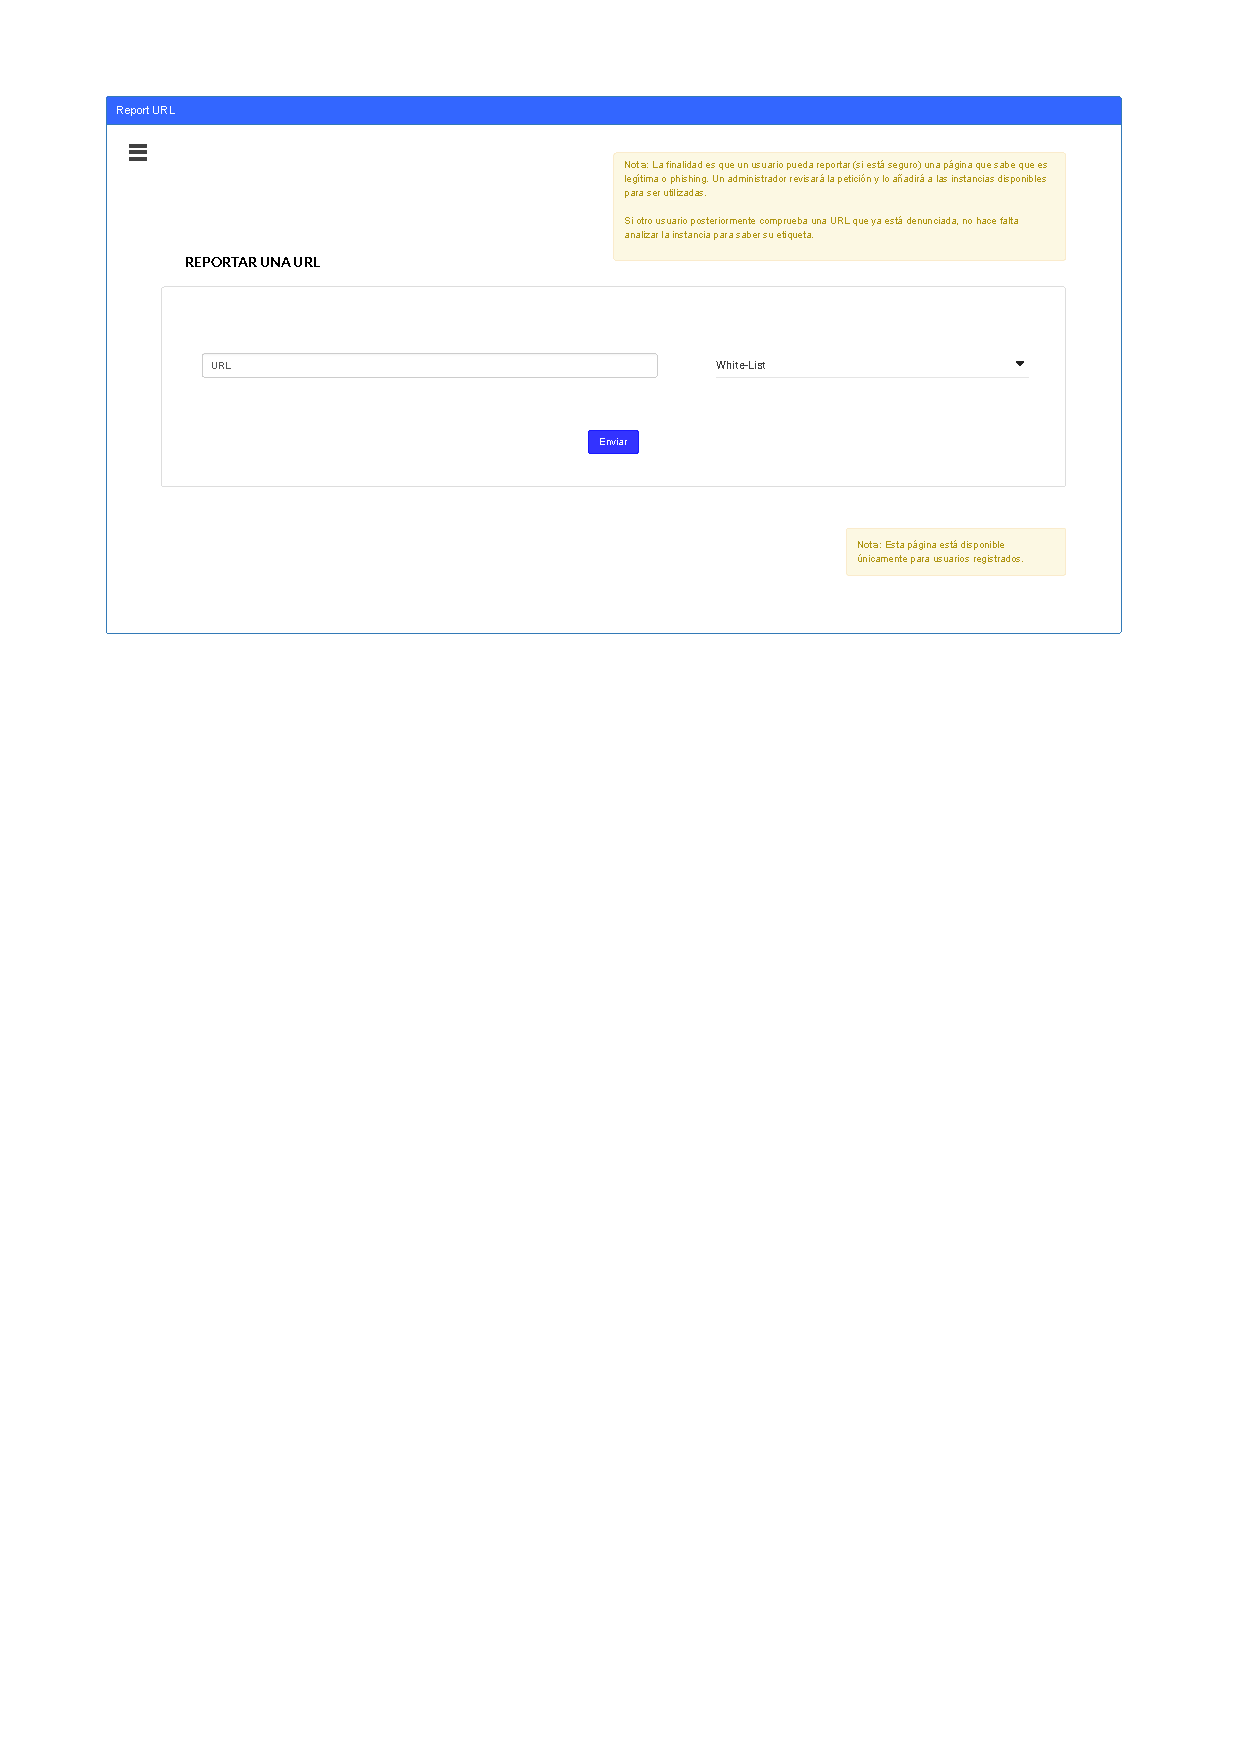
\includegraphics[width=\textwidth]{../img/anexos/mockups/3-mockups-report_url}
	\label{mock:report_url}
\end{figure}

\begin{figure}[h]
	\caption{Prototipos: perfil del usuario}
	\centering
	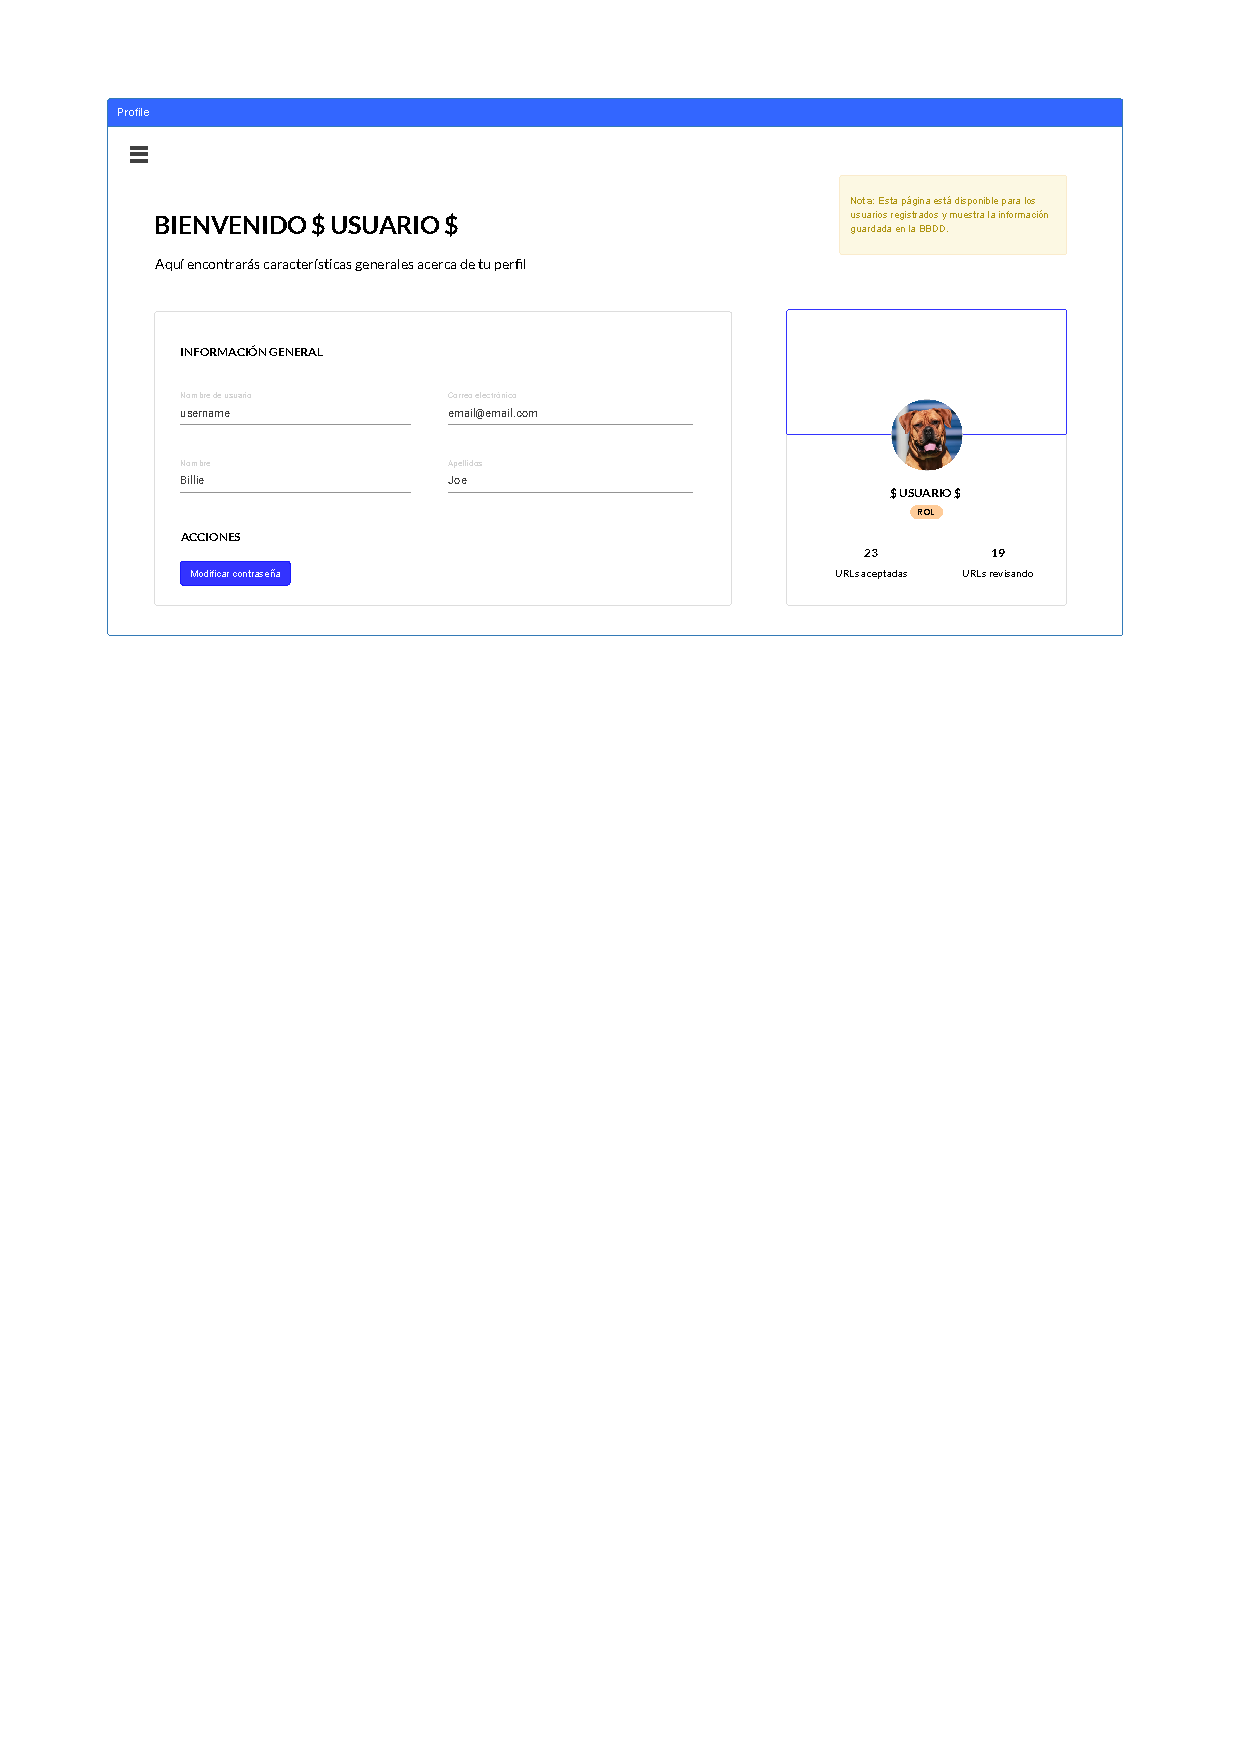
\includegraphics[width=\textwidth]{../img/anexos/mockups/4-mockups-profile}
	\label{mock:profile}
\end{figure}

\begin{figure}[h]
	\caption{Prototipos: administración de modelos}
	\centering
	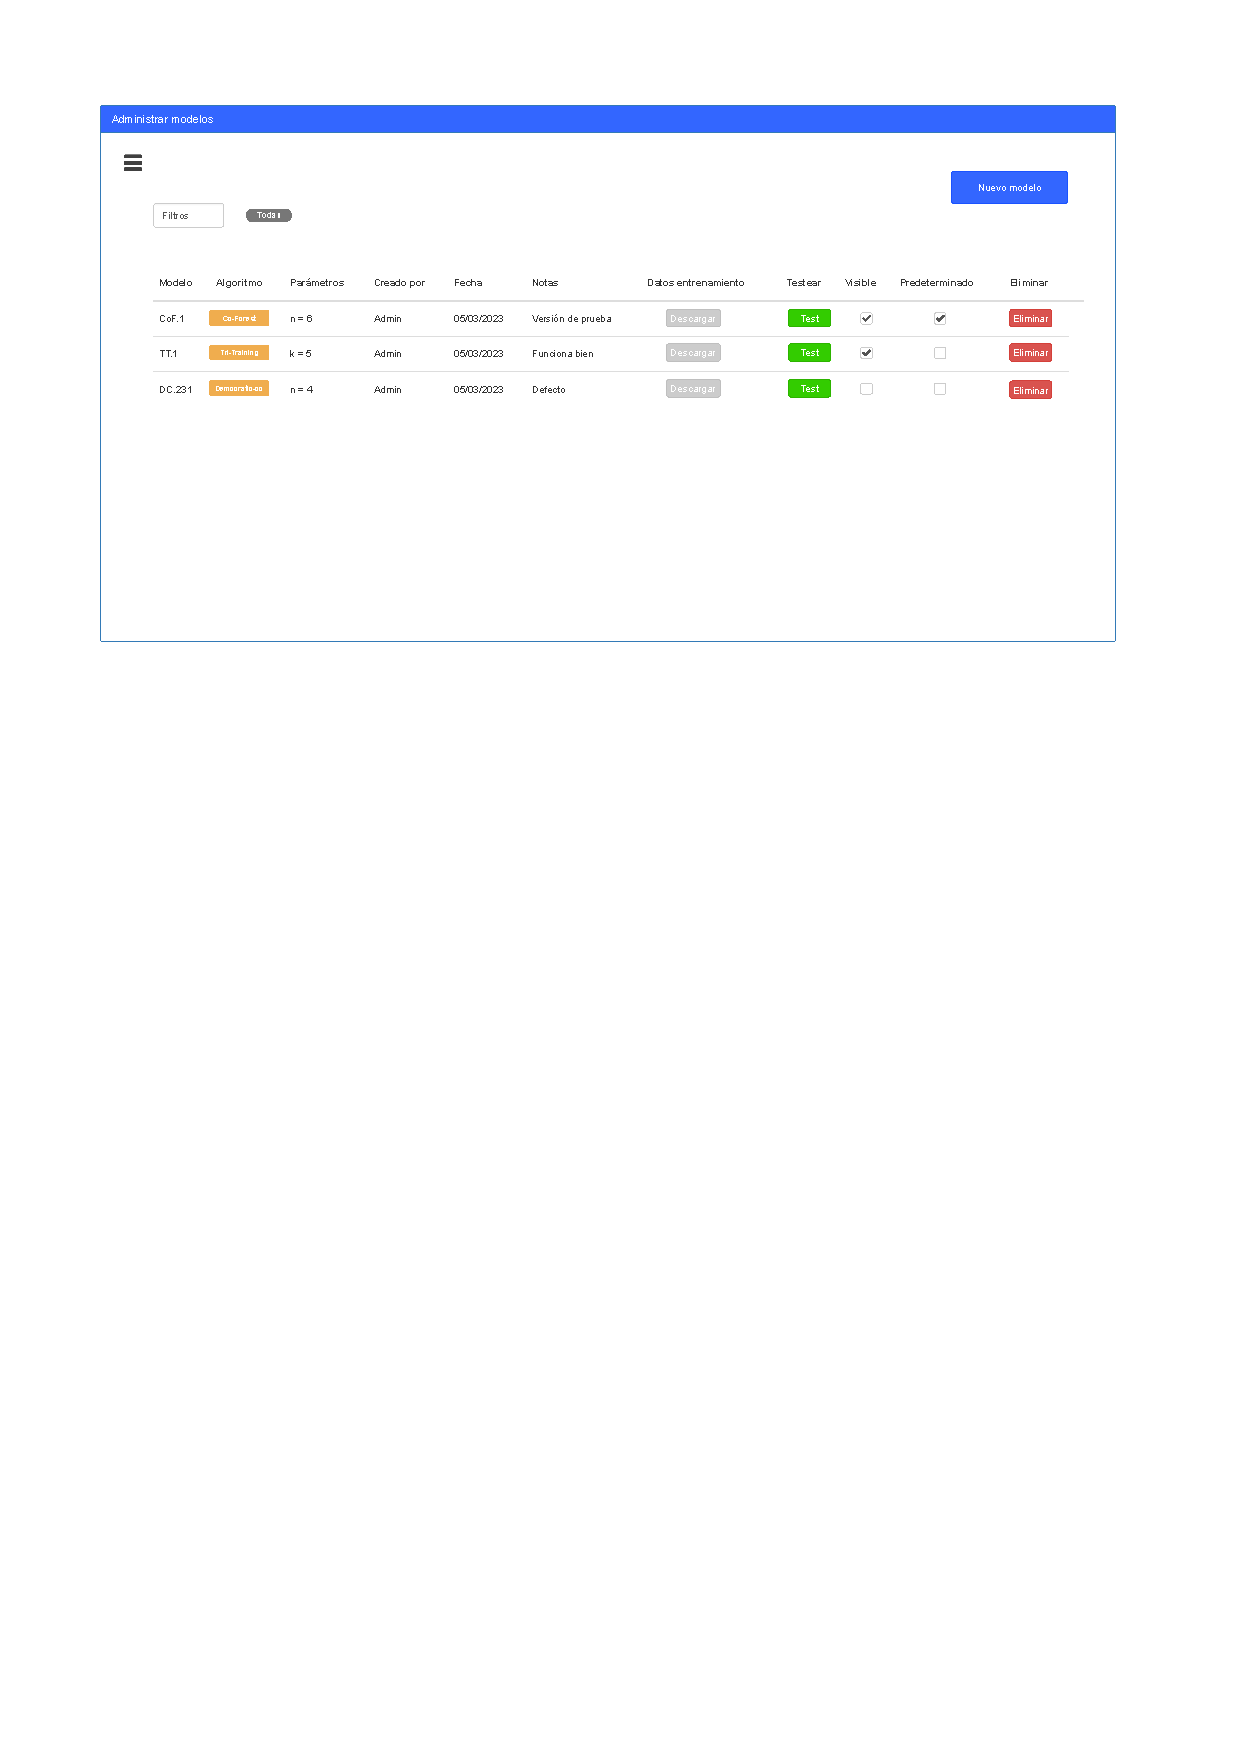
\includegraphics[width=\textwidth]{../img/anexos/mockups/5-mockups-models}
	\label{mock:model-admin}
\end{figure}

\begin{figure}[h]
	\caption{Prototipos: creación de modelos}
	\centering
	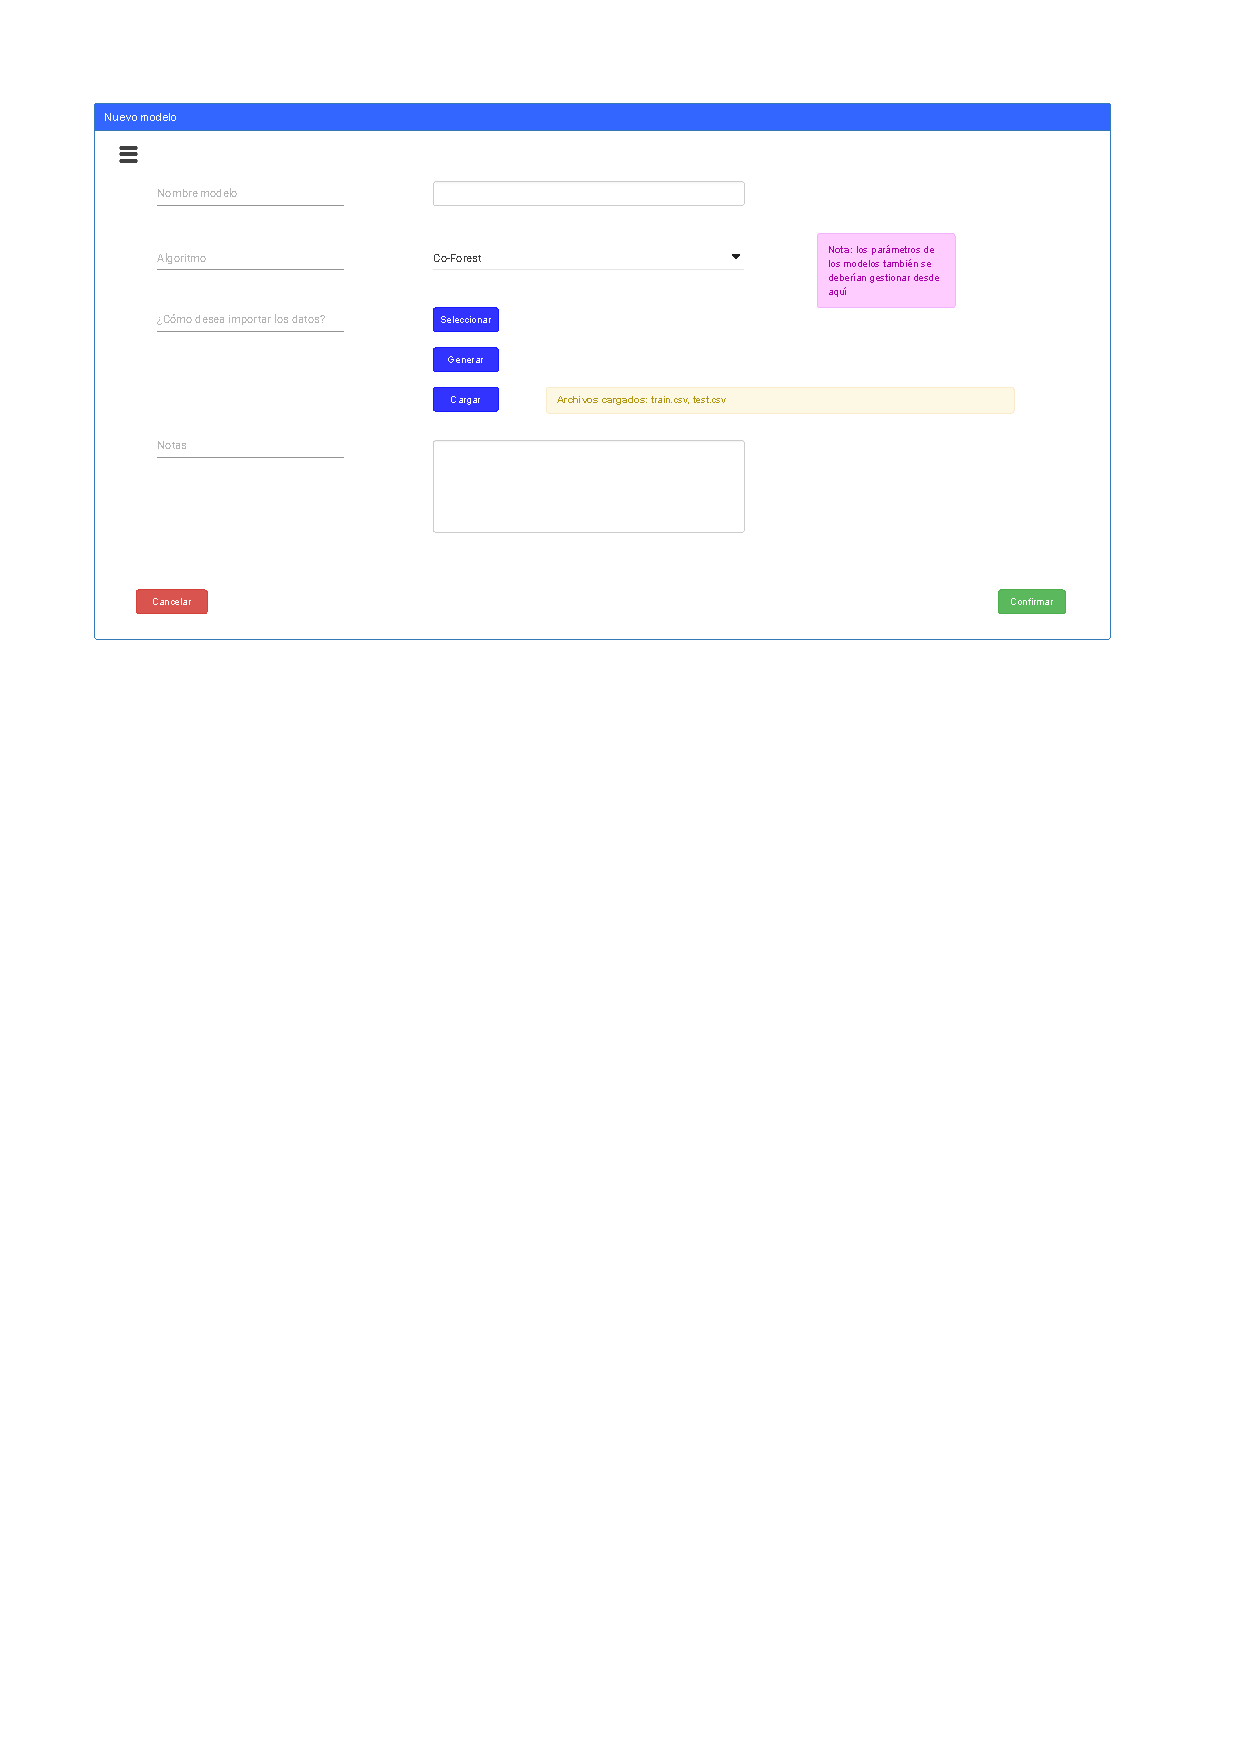
\includegraphics[width=\textwidth]{../img/anexos/mockups/6-mockups-new_model}
	\label{mock:model-new}
\end{figure}

\begin{figure}[h]
	\caption{Prototipos: evaluación de modelos}
	\centering
	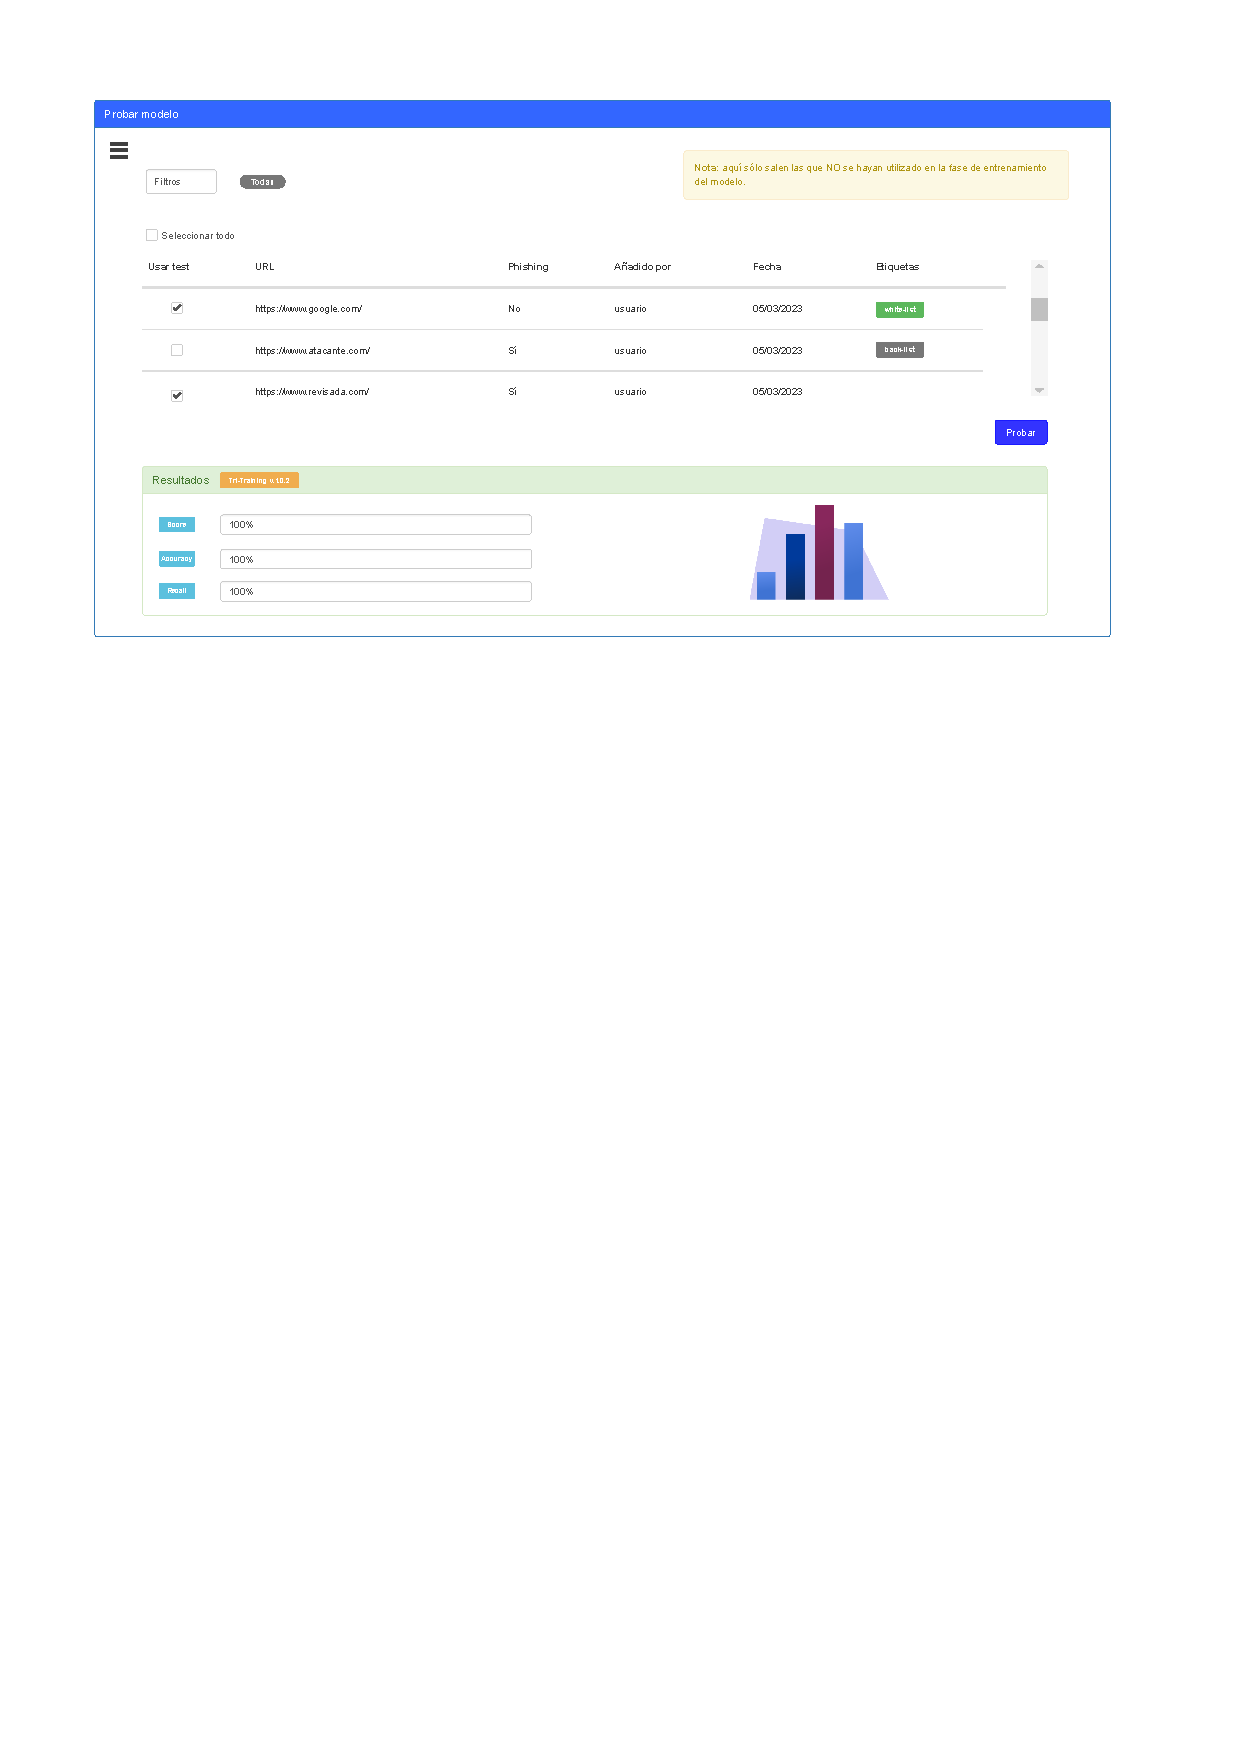
\includegraphics[width=\textwidth]{../img/anexos/mockups/7-mockups-test_model}
	\label{mock:model-test}
\end{figure}

\begin{figure}[h]
	\caption{Prototipos: selección de instancias}
	\centering
	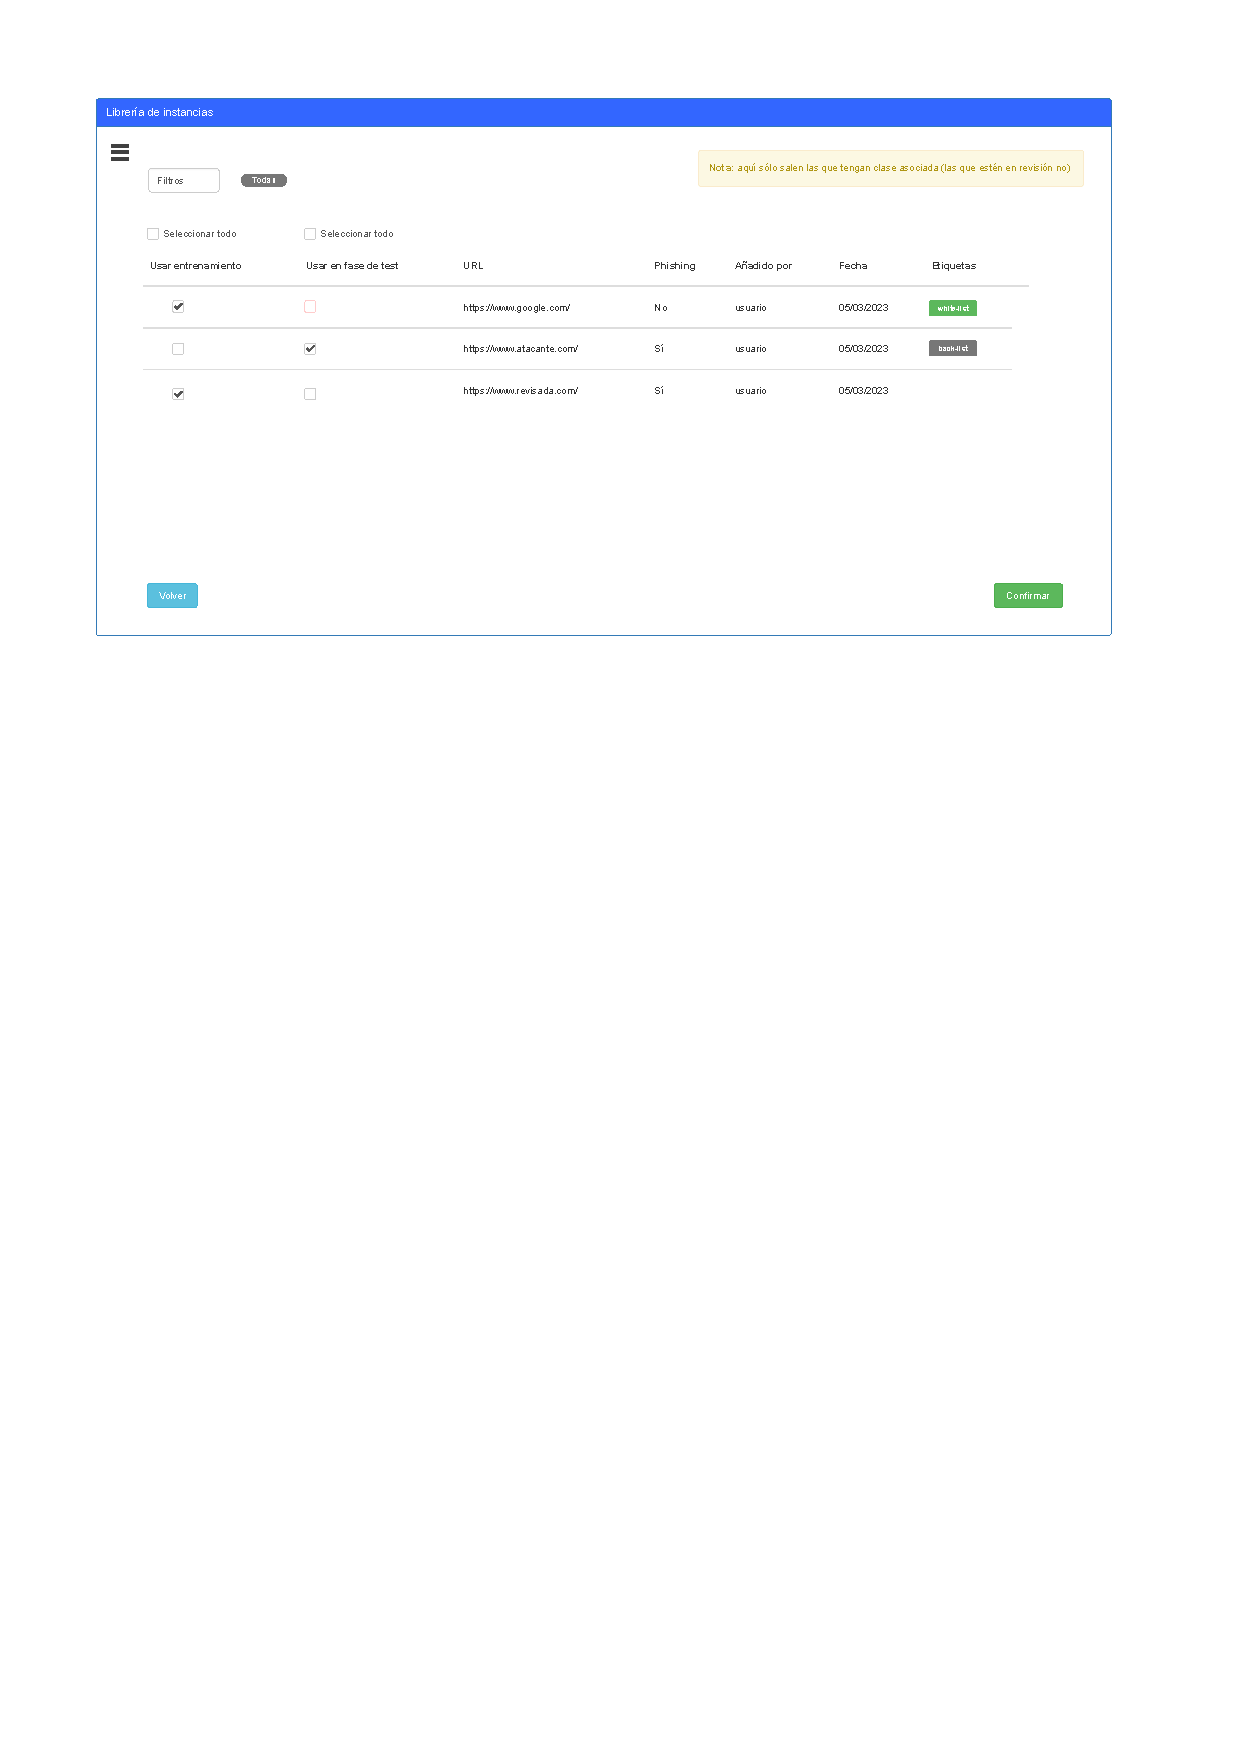
\includegraphics[width=\textwidth]{../img/anexos/mockups/8-mockups-select_instances}
	\label{mock:instance-selection}
\end{figure}

\begin{figure}[h]
	\caption{Prototipos: administración de instancias}
	\centering
	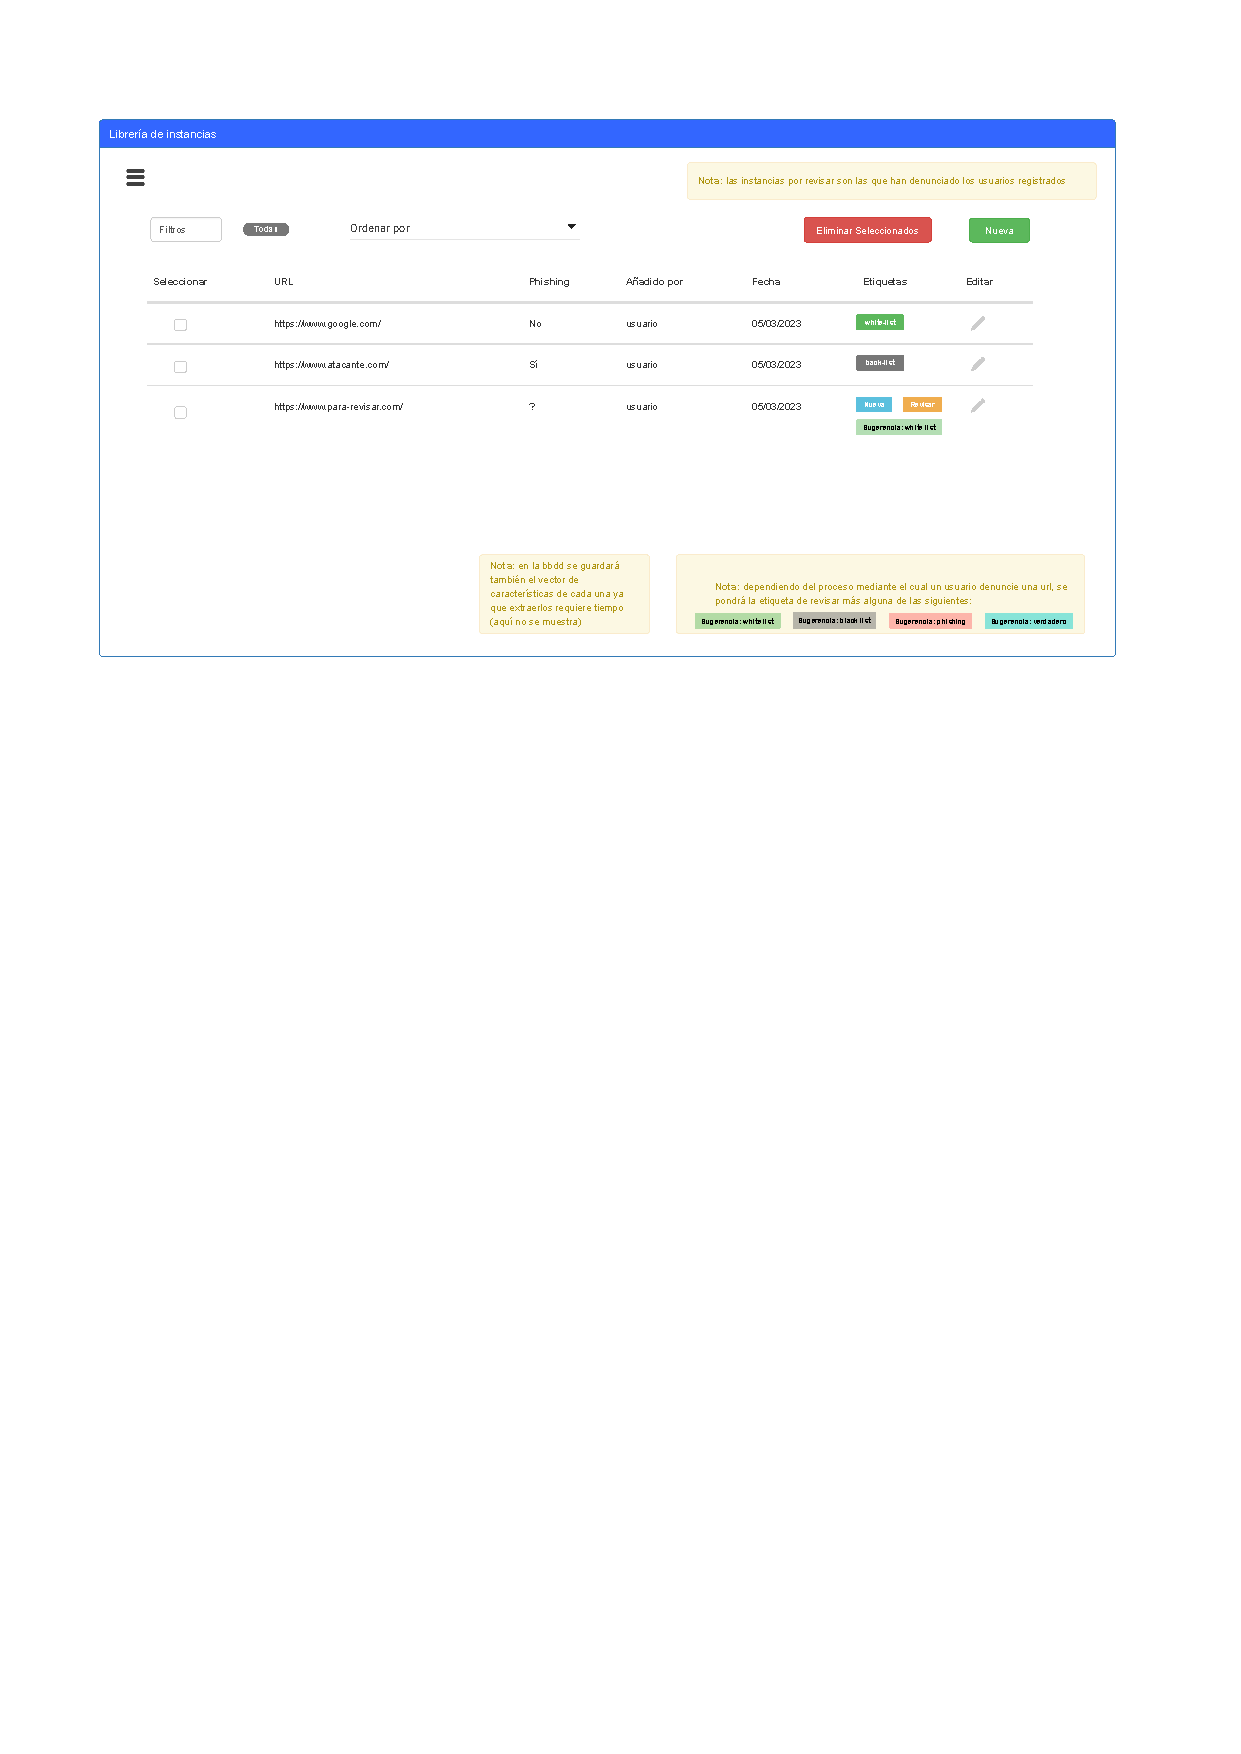
\includegraphics[width=\textwidth]{../img/anexos/mockups/9-mockups-instances}
	\label{mock:instance-admin}
\end{figure}

\begin{figure}[h]
	\caption{Prototipos: edición de instancias}
	\centering
	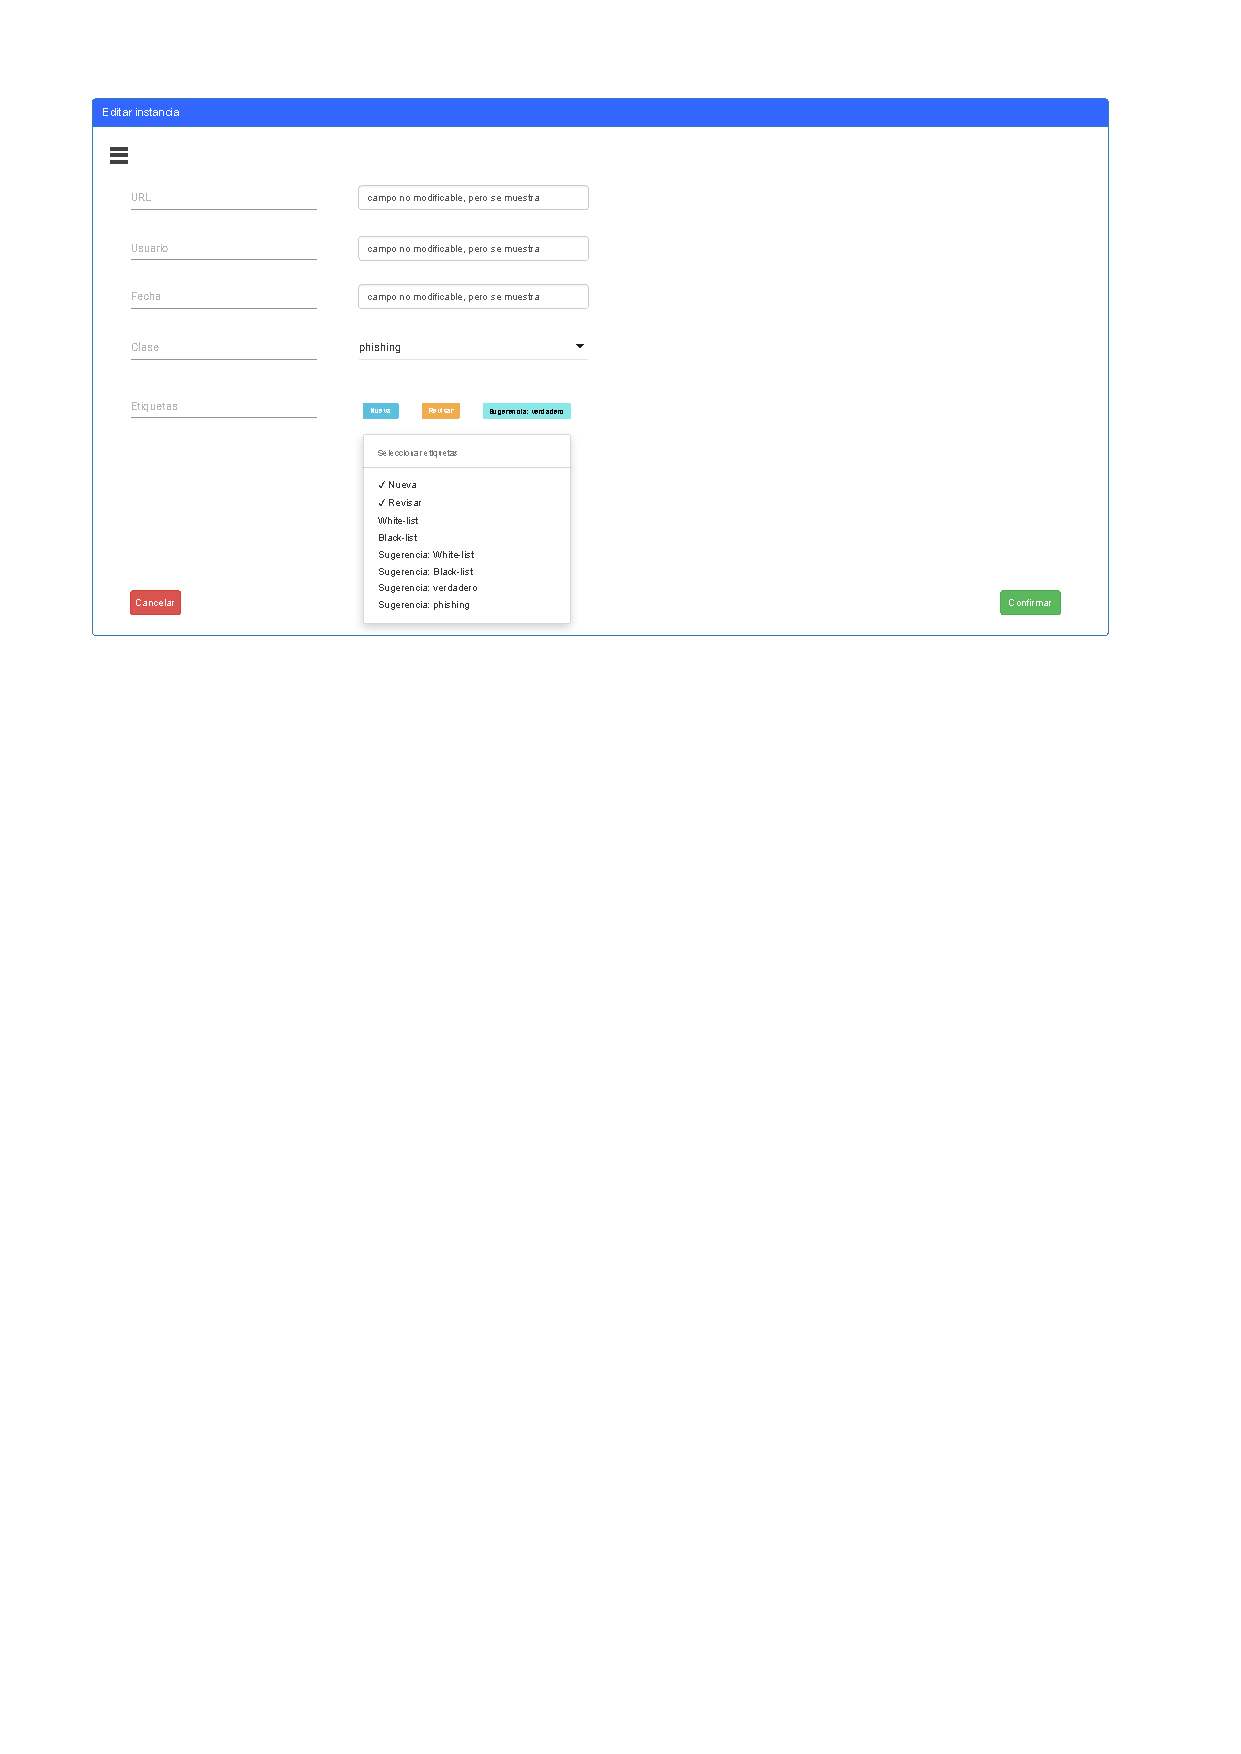
\includegraphics[width=\textwidth]{../img/anexos/mockups/10-mockups-edit_instance}
	\label{mock:instances-edit}
\end{figure}


\section{Especificación de requisitos}
\label{s:requisitos}

Se detalla a continuación la especificación de requisitos tradicional de la aplicación \textit{web} propuesta basada en el catálogo de requisitos de la sección~\ref{s:cat-requisitos}.

\subsection{Diagrama de casos de uso}
\label{ss:diagrama-casos-uso}

Partiendo de las historias de usuario extraídas en las entrevistas realizadas con el \textit{product owner} y de los \textit{mockups} mostrados en la sección~\ref{s:mockups}, se ha extraído el diagrama de casos de uso disponible en la figura~\ref{b:diagrama-cu}.

\begin{figure}[h]
	\caption{Diagramas: casos de uso}
	\centering
	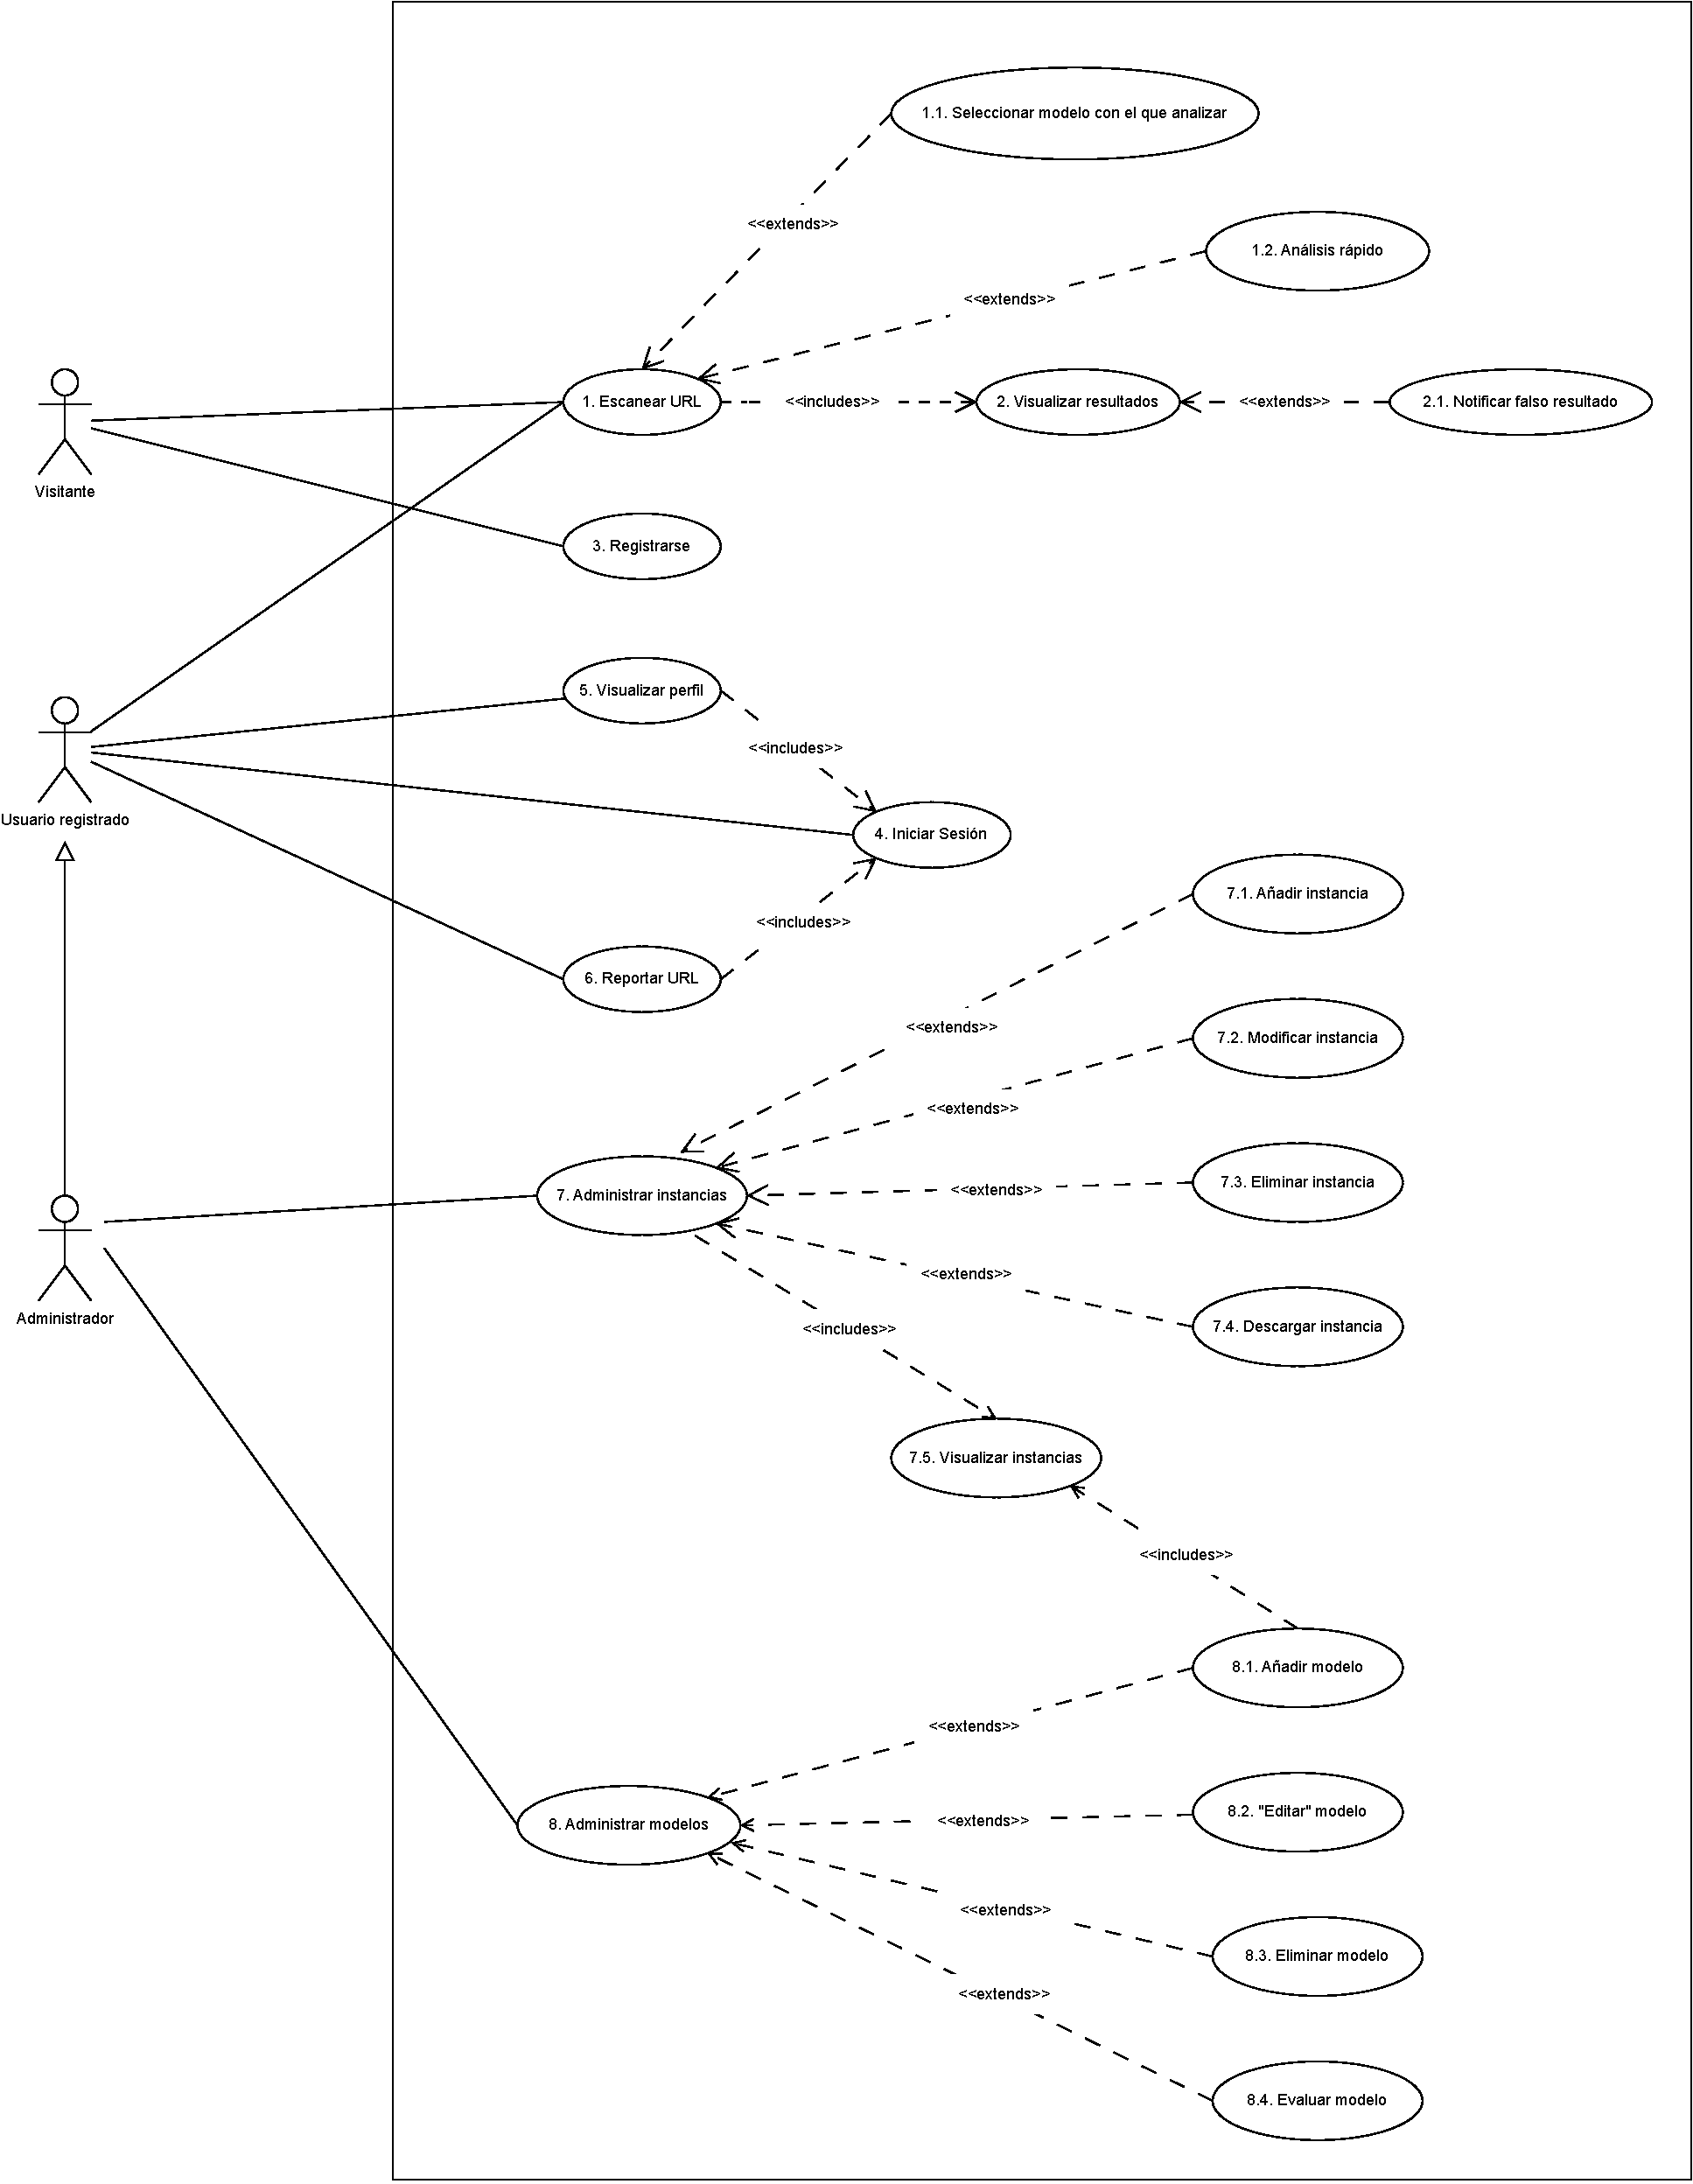
\includegraphics[width=\textwidth]{../img/anexos/diagrams/cu}
	\label{b:diagrama-cu}
\end{figure}

A continuación se muestra la tabla correspondiente a cada caso de uso.

% Caso de Uso 1 -> Escanear URL
\begin{table}[p]
	\centering
	\begin{tabularx}{\linewidth}{ p{0.21\columnwidth} p{0.71\columnwidth} }
		\toprule
		\textbf{CU-1}    & \textbf{Escanear URL}\\
		\toprule
		\textbf{Versión}              & 1.0    \\
		\textbf{Autor}                & Patricia Hernando Fernández \\
		\textbf{Requisitos asociados} & RF-xx, RF-xx \\
		\textbf{Descripción}          & Permitir que un usuario realice un escaneo de la URL que desee. Para ello, seleccionará los modelos que considere adecuados y se mostrarán los resultados en un \textit{dashboard} (CU-2 en la tabla~\ref{cu:visualizar-resultados}). \\
		\textbf{Precondición}         & No hay precondiciones. \\
		\textbf{Acciones}             &
		\begin{enumerate}
			\def\labelenumi{\arabic{enumi}.}
			\tightlist
			\item El usuario introduce la URL.
			\item El usuario selecciona los modelos de ML que considere (consultar CU-1.1 en la tabla~\ref{cu:seleccionar-modelos-ml}).
			\item El usuario decide si quiere realizar un análisis rápido.
			\item El usuario pulsa el botón de <<realizar análisis>>.
		\end{enumerate}\\
		\textbf{Postcondición}        & No hay postcondiciones. \\
		\textbf{Excepciones}          & En caso de que la URL introducida sea inalcanzable (tras aplicar reintentos) o que no haya ningún modelo disponible, el usuario será notificado y redirigido a la página principal. \\
		\textbf{Importancia}          & Alta \\
		\bottomrule
	\end{tabularx}
	\caption{CU-1 Escanear URL.}
	\label{cu:escanear-url}
\end{table}


% Caso de Uso 1.1 -> Seleccionar modelos
\begin{table}[p]
	\centering
	\begin{tabularx}{\linewidth}{ p{0.21\columnwidth} p{0.71\columnwidth} }
		\toprule
		\textbf{CU-1.1}    & \textbf{Seleccionar modelos con los que analizar}\\
		\toprule
		\textbf{Versión}              & 2.0    \\
		\textbf{Autor}                & Patricia Hernando Fernández \\
		\textbf{Requisitos asociados} & RF-xx, RF-xx \\
		\textbf{Descripción}          & Se mostrará al usuario los distintos modelos disponibles (y visibles) para que elija los que desee. \\
		\textbf{Precondición}         & Estar realizando el CU-1 (disponible en la tabla~\ref{cu:escanear-url}). \\
		\textbf{Acciones}             &
		\begin{enumerate}
			\def\labelenumi{\arabic{enumi}.}
			\tightlist
			\item Se cargan los modelos disponibles en la base de datos.
			\item El usuario selecciona los modelos que quiera utilizar.
		\end{enumerate}\\
		\textbf{Postcondición}        & Los modelos seleccionados quedan guardados. \\
		\textbf{Excepciones}          & En caso de no haber modelos disponibles la lista quedará vacía y se controlará la excepción en el CU-1 (tabla~\ref{cu:escanear-url}). \\
		\textbf{Importancia}          & Baja \\
		\bottomrule
	\end{tabularx}
	\caption{CU-1.1 Seleccionar modelos con los que analizar.}
	\label{cu:seleccionar-modelos-ml}
\end{table}

% Caso de Uso 2 -> Visualizar resultados
\begin{table}[p]
	\centering
	\begin{tabularx}{\linewidth}{ p{0.21\columnwidth} p{0.71\columnwidth} }
		\toprule
		\textbf{CU-2}    & \textbf{Visualizar resultados}\\
		\toprule
		\textbf{Versión}              & 1.0    \\
		\textbf{Autor}                & Patricia Hernando Fernández \\
		\textbf{Requisitos asociados} & RF-xx, RF-xx \\
		\textbf{Descripción}          & Se muestra al usuario los resultados tras haber analizado la URL mediante los algoritmos de ML seleccionados. Para ello se hará uso de un \textit{dashboard}, donde además se podrá notificar un falso resultado (CU-2.1 en la tabla~\ref{cu:notificar-falso-resultado}).\\
		\textbf{Precondición}         & Haber realizado un análisis previamente (CU-1 en la tabla~\ref{cu:escanear-url}). \\
		\textbf{Acciones}             &
		\begin{enumerate}
			\def\labelenumi{\arabic{enumi}.}
			\tightlist
			\item El usuario es redirigido a un \textit{dashboard}.
			\item El usuario puede interactuar con los distintos gráficos y la información mostrada en la página.
			\item El usuario puede notificar si considera que el análisis es erróneo (CU-2.1 en la tabla~\ref{cu:notificar-falso-resultado}).
		\end{enumerate}\\
		\textbf{Postcondición}        & No hay postcondiciones \\
		\textbf{Excepciones}          & En caso de intentar acceder al \textit{dashboard} sin haber realizado un análisis previo, el usuario será redirigido a la página principal con un mensaje informativo.\\
		\textbf{Importancia}          & Alta \\
		\bottomrule
	\end{tabularx}
	\caption{CU-2 Visualizar resultados.}
	\label{cu:visualizar-resultados}
\end{table}


% Caso de Uso 2.1 -> Notificar falso resultado
\begin{table}[p]
	\centering
	\begin{tabularx}{\linewidth}{ p{0.21\columnwidth} p{0.71\columnwidth} }
		\toprule
		\textbf{CU-2.1}    & \textbf{Notificar falso resultado}\\
		\toprule
		\textbf{Versión}              & 1.0    \\
		\textbf{Autor}                & Patricia Hernando Fernández \\
		\textbf{Requisitos asociados} & RF-xx, RF-xx \\
		\textbf{Descripción}          & Permite a un usuario notificar automáticamente a la aplicación si considera que el resultado de un análisis es erróneo.\\
		\textbf{Precondición}         & Encontrarse en el \textit{dashboard} tras un análisis (CU-2 en la tabla~\ref{cu:visualizar-resultados}) y haber iniciado sesión (CU-4 en la tabla~\ref{cu:iniciar-sesion}).\\
		\textbf{Acciones}             &
		\begin{enumerate}
			\def\labelenumi{\arabic{enumi}.}
			\tightlist
			\item El usuario pulsa el botón <<notificar falso resultado>>.
		\end{enumerate}\\
		\textbf{Postcondición}        & Se registra la URL notificada en la base de datos con el campo <<sugerencia>> establecido al valor opuesto del resultado mostrado. \\
		\textbf{Excepciones}          & Si el usuario no ha iniciado sesión, será informado de que la notificación no ha sido realizada por este motivo. En caso de errores con la base de datos se controlarán y se informará al usuario de la notificación no realizada.\\
		\textbf{Importancia}          & Baja \\
		\bottomrule
	\end{tabularx}
	\caption{CU-2.1  Notificar falso resultado.}
	\label{cu:notificar-falso-resultado}
\end{table}


% Caso de Uso 3 -> Registrarse
\begin{table}[p]
	\centering
	\begin{tabularx}{\linewidth}{ p{0.21\columnwidth} p{0.71\columnwidth} }
		\toprule
		\textbf{CU-3}    & \textbf{Registrarse}\\
		\toprule
		\textbf{Versión}              & 1.0    \\
		\textbf{Autor}                & Patricia Hernando Fernández \\
		\textbf{Requisitos asociados} & RF-xx, RF-xx \\
		\textbf{Descripción}          & Permite a un usuario crear una cuenta en la aplicación.\\
		\textbf{Precondición}         & El usuario no debe estar registrado ni haber iniciado sesión (CU-4 en la tabla~\ref{cu:iniciar-sesion}). \\
		\textbf{Acciones}             &
		\begin{enumerate}
			\def\labelenumi{\arabic{enumi}.}
			\tightlist
			\item El usuario selecciona <<Registrarse>>.
			\item El usuario introduce el nombre de usuario que considere.
			\item El usuario introduce un \textit{email} asociado a la cuenta.
			\item El usuario introduce la contraseña deseada.
			\item El usuario pulsa el botón de <<Registrar>>.
		\end{enumerate}\\
		\textbf{Postcondición}        & La información del nuevo usuario queda almacenada en la base de datos. \\
		\textbf{Excepciones}          & En caso de que los datos estén repetidos o el \textit{email} sea incorrecto, se pedirá al usuario que corrija los errores y no se creará la nueva cuenta. Si hay un usuario \textit{logueado} será redirigido a la página principal con un mensaje informativo.\\
		\textbf{Importancia}          & Media \\
		\bottomrule
	\end{tabularx}
	\caption{CU-3 Registrarse.}
	\label{cu:registrarse}
\end{table}


% Caso de Uso 4 -> Iniciar sesión
\begin{table}[p]
	\centering
	\begin{tabularx}{\linewidth}{ p{0.21\columnwidth} p{0.71\columnwidth} }
		\toprule
		\textbf{CU-4}    & \textbf{Iniciar sesión}\\
		\toprule
		\textbf{Versión}              & 1.0    \\
		\textbf{Autor}                & Patricia Hernando Fernández \\
		\textbf{Requisitos asociados} & RF-xx, RF-xx \\
		\textbf{Descripción}          & Permite a un usuario iniciar sesión en la aplicación.\\
		\textbf{Precondición}         & El usuario no debe haber iniciado sesión en el navegador (CU-4 en la tabla~\ref{cu:iniciar-sesion}). \\
		\textbf{Acciones}             &
		\begin{enumerate}
			\def\labelenumi{\arabic{enumi}.}
			\tightlist
			\item El usuario pulsa el botón de <<Iniciar sesión>>.
			\item El usuario introduce el nombre de usuario asociado a su cuenta.
			\item El usuario introduce la contraseña asociada a la cuenta.
			\item El usuario pulsa el botón de <<Iniciar sesión>>.
		\end{enumerate}\\
		\textbf{Postcondición}        & La información del usuario queda cargada en las variables de sesión. \\
		\textbf{Excepciones}          & En caso de que los datos sean incorrectos el usuario será notificado. Si hay un usuario \textit{logueado} será redirigido a la página principal con un mensaje informativo.\\
		\textbf{Importancia}          & Media \\
		\bottomrule
	\end{tabularx}
	\caption{CU-3 Iniciar sesión.}
	\label{cu:iniciar-sesion}
\end{table}

% Caso de Uso 5 -> Reportar URL
\begin{table}[p]
	\centering
	\begin{tabularx}{\linewidth}{ p{0.21\columnwidth} p{0.71\columnwidth} }
		\toprule
		\textbf{CU-5}    & \textbf{Reportar URL}\\
		\toprule
		\textbf{Versión}              & 1.0    \\
		\textbf{Autor}                & Patricia Hernando Fernández \\
		\textbf{Requisitos asociados} & RF-xx, RF-xx \\
		\textbf{Descripción}          & Permite a un usuario reportar una
		URL si considera que pertenece a una lista blanca o a una lista negra.\\
		\textbf{Precondición}         & El usuario debe de haber iniciado sesión (CU-4 en la tabla~\ref{cu:iniciar-sesion}). \\
		\textbf{Acciones}             &
		\begin{enumerate}
			\def\labelenumi{\arabic{enumi}.}
			\tightlist
			\item El usuario introduce la URL a reportar.
			\item El usuario selecciona el tipo de lista a la que pertenece la URL.
			\item El usuario pulsa el botón de <<Enviar>>.
		\end{enumerate}\\
		\textbf{Postcondición}        & Se registra la URL reportada en la base de datos con el campo <<sugerencia>> establecido al valor seleccionado en el desplegable (ejemplo: \textit{white-list}). \\
		\textbf{Excepciones}          & En caso de no haber iniciado sesión, el usuario será redirigido a una pantalla especial (error 403, acceso restringido) con un enlace para iniciar sesión. Se controla en aplicación que el usuario haya rellenado todos los campos necesarios. \\
		\textbf{Importancia}          & Baja \\
		\bottomrule
	\end{tabularx}
	\caption{CU-5 Reportar URL.}
	\label{cu:reportar-url}
\end{table}



\apendice{Especificación de diseño}
\label{s:anexo-C}

\section{Introducción}

La especificación de diseño es una descripción detallada de la estructura, el comportamiento y la interacción de los componentes de un producto \textit{software}. Se muestran a continuación dichos apartados para la aplicación desarrollada en este proyecto.

\section{Diseño de datos}
\label{s:diseno-datos}
A continuación se expone el procedimiento seguido para desarrollar el diseño de datos de la aplicación.

Para implementar la persistencia, se ha decidido utilizar una base de datos PostgreSQL (debido a la compatibilidad con Heroku y a su carácter \textit{open-source}). El diseño de la misma ha pasado por diversas fases: el diseño del modelo entidad-relación (disponible en la subsección~\ref{c:diagrama_entidad_relacion}), el diseño del diagrama relacional (subsección~\ref{c:diagrama_relacional}) y, por último, el diccionario de datos (subsección~\ref{c:diccionario_datos}).


\subsection{Modelo entidad-relación}
\label{c:diagrama_entidad_relacion}

Para analizar las posibles relaciones entre entidades, se ha hecho uso del diagrama E-R disponible en la imagen~\ref{c:diagrama-er}. Como se puede observar, ambas ISAs son exclusivas totales (es decir, todos los elementos pertenecen a una y solo una subclase).

Son destacables dos aspectos dentro del diagrama: la aparición de <<bucles>> y una relación ternaria. La relación ternaria se debe a la posibilidad de que un mismo usuario reporte más de una vez la misma URL en distintas fechas (se ha de mantener un historial). Por otro lado (y tras haberlo consultado con el profesor Jesús Maudes), los <<bucles>> se han permitido debido a que, en este caso, los extremos aportan información y realizan roles muy distintos.

En el primero (relaciones <<reporta>> y <<revisa>>), un administrador debe revisar todas las instancias reportadas por cualquier usuario. En un lado, el rol desempeñado sería <<reportar una URL>>, mientras que en el otro, sería <<revisarla>> y aceptarla (aporta nueva información, el usuario que reporta es distinto del que revisa). En el segundo (relaciones <<administra>>, <<revisa>> y <<se entrena>>) nuevamente hay una gran independencia en el rol desempeñado. Por ejemplo, para que un modelo se entrene con una instancia, debe de estar revisada por un administrador. Evidentemente este modelo va a ser gestionado por otro, pero es independiente de las acciones anteriores.

\subsection{Diagrama relacional}
\label{c:diagrama_relacional}

Partiendo del modelo E-R disponible en la figura~\ref{c:diagrama-er}, se ha diseñado el diagrama relacional disponible en la imagen~\ref{c:diagrama-relacional}.

A continuación se van a mencionar algunas de las decisiones de implementación tomadas. Sin embargo, el desarrollo completo de por qué se ha tomado cada una y todos los detalles se encuentran disponibles en el diccionario de datos de la sección~\ref{c:diccionario_datos}.

Respecto a la ISA existente en la entidad \texttt{Users}, se ha decidido implementar en una única tabla debido a que resulta útil para los desarrolladores contar con el discriminante como campo de tabla y, además, únicamente hay un atributo extra para los usuarios <<estándar>> (que son la mayoría, por lo que la pérdida de espacio es completamente despreciable). En cuanto a la ISA en la entidad \texttt{Models}, se ha implementado considerando que es una interrelación 1:1 debido a que cada subclase tiene atributos muy distintos.

Por otro lado, se ha omitido la entidad \texttt{Date} ya que este es uno de los casos en los que no merece la pena que pase a ser tabla por no aportar información extra (resulta indiferente contar con una clase o con un \textit{timestamp}). Aún así, formará parte de la clave primaria (\texttt{PK}) en la relación.

Para facilitar el desarrollo y reducir errores derivados de posibles equivocaciones, se han decorado los atributos con un prefijo. De este modo, por ejemplo, el identificador de la tabla \texttt{Available\_instances} pasará a llamarse \texttt{instance\_id}. Además, también se ha añadido el prefijo \textit{available} a ciertas clases para que sea más evidente la diferencia entre los propios objetos del sistema y la información almacenada en la base de datos.


\begin{landscape}
\begin{figure}[h]
	\caption[Diagrama: entidad-relación]{Diagrama entidad relación de la aplicación}
	\centering
	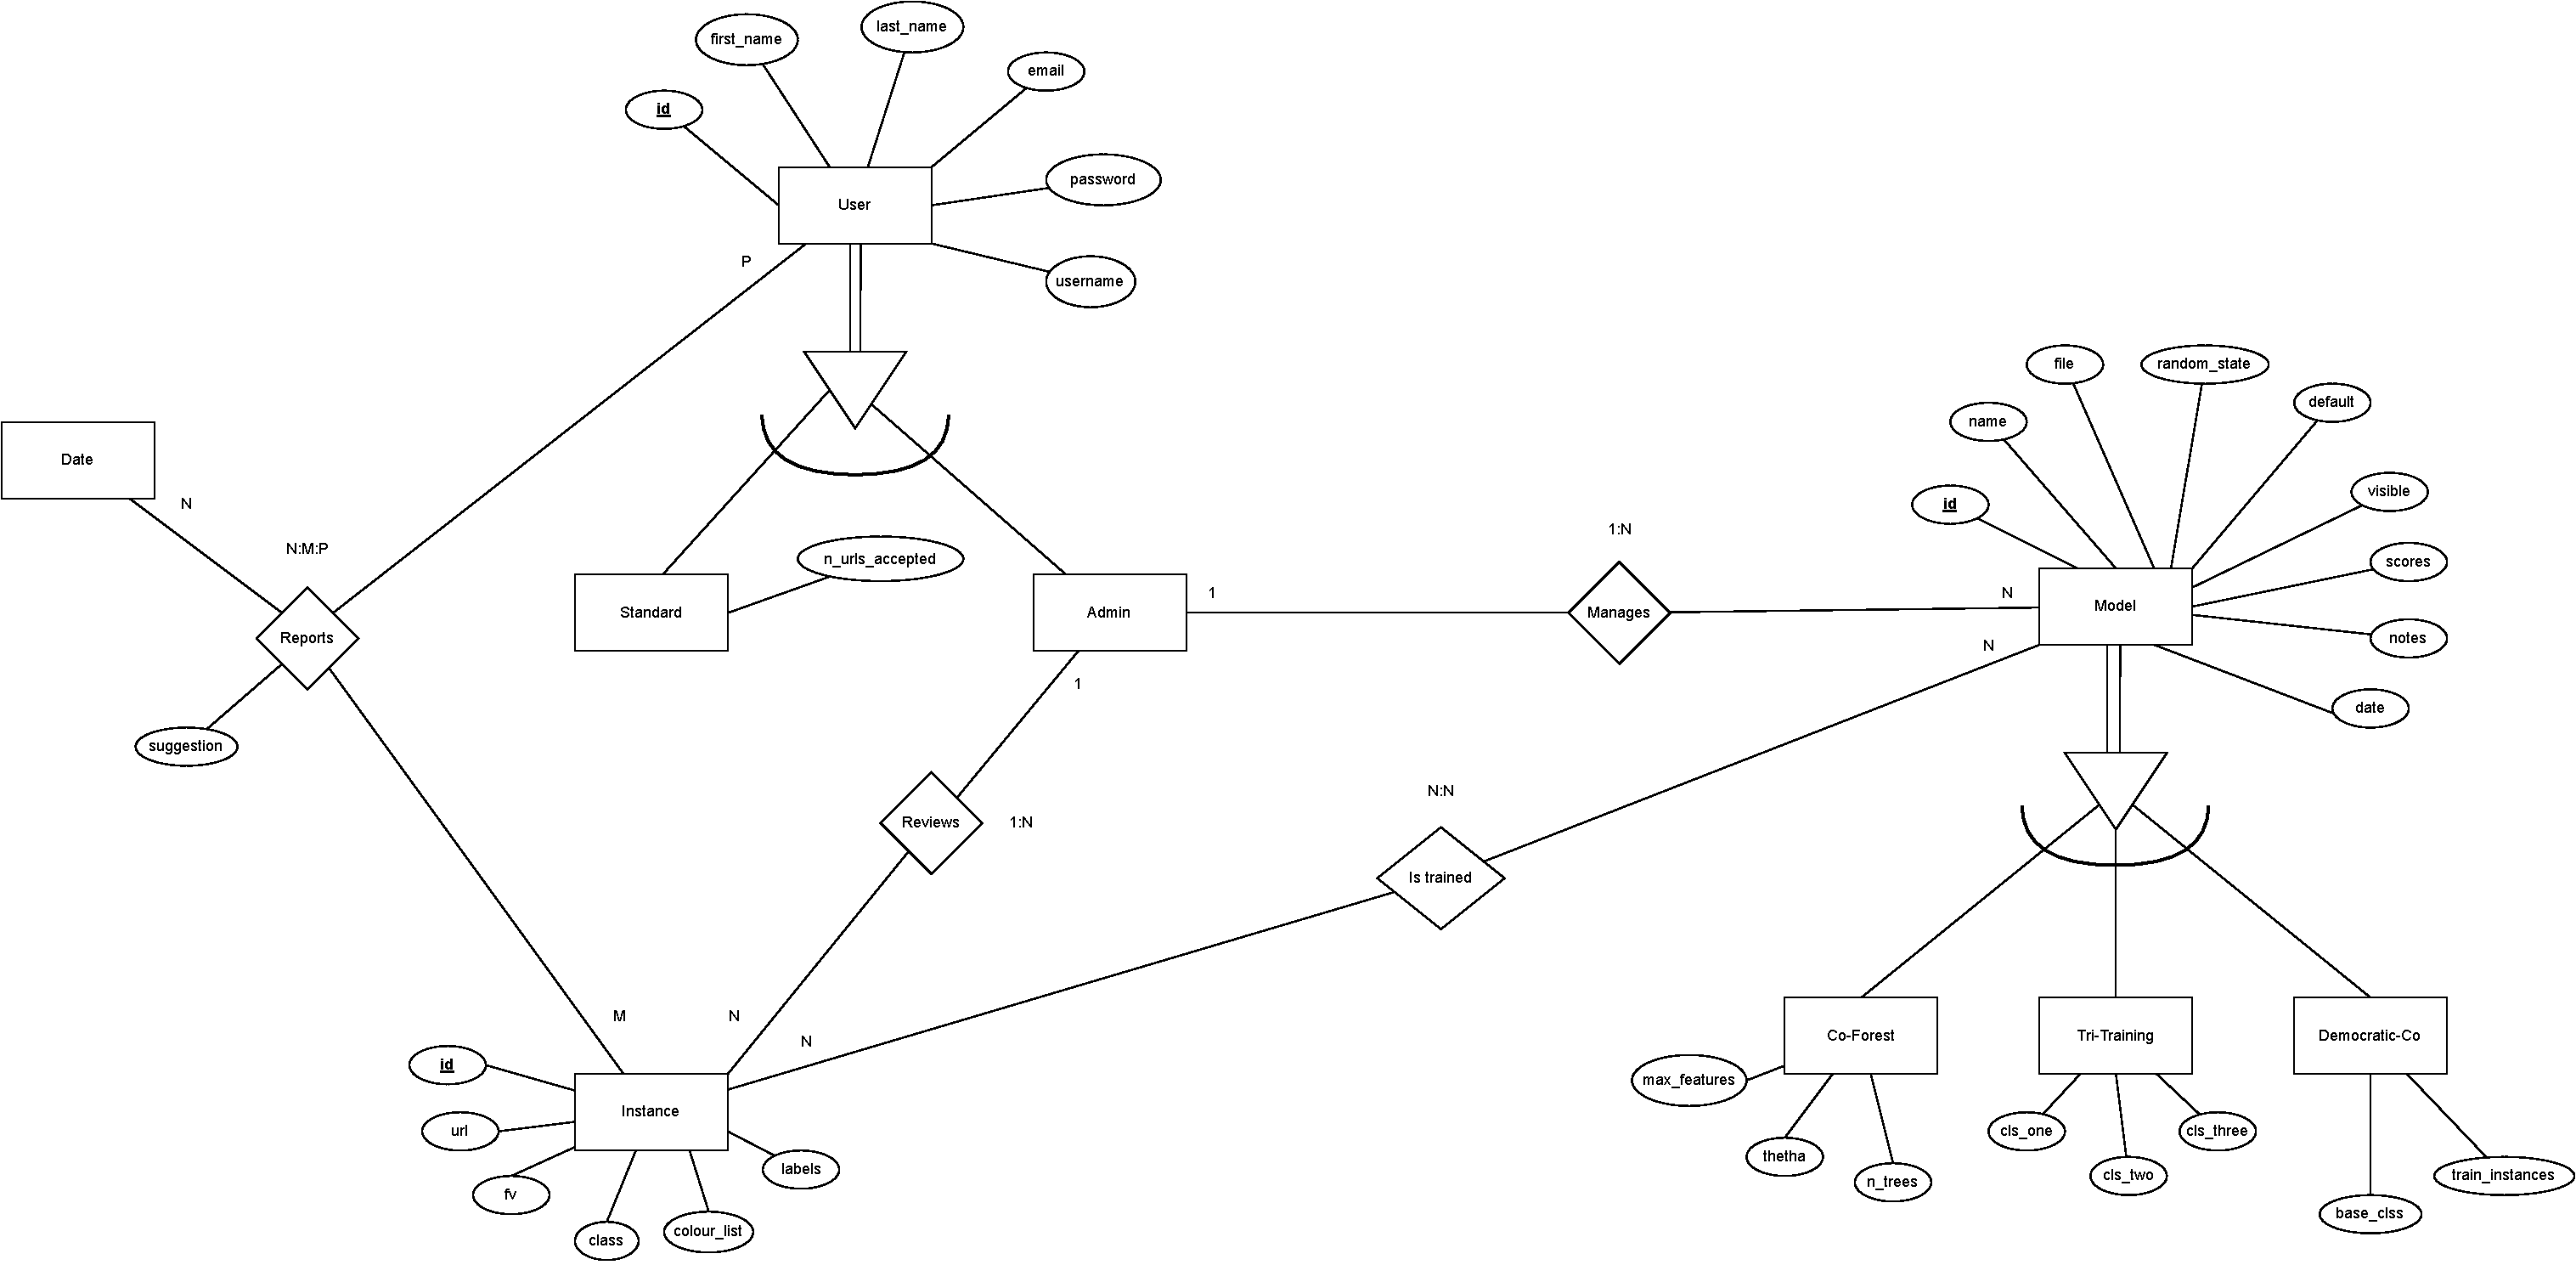
\includegraphics[scale=0.4]{../img/anexos/diagrams/er}
	\label{c:diagrama-er}
\end{figure}
\end{landscape}

\begin{landscape}
	\begin{figure}[h]
		\caption[Diagrama: relacional]{Diagrama relacional de la base de datos}
		\centering
		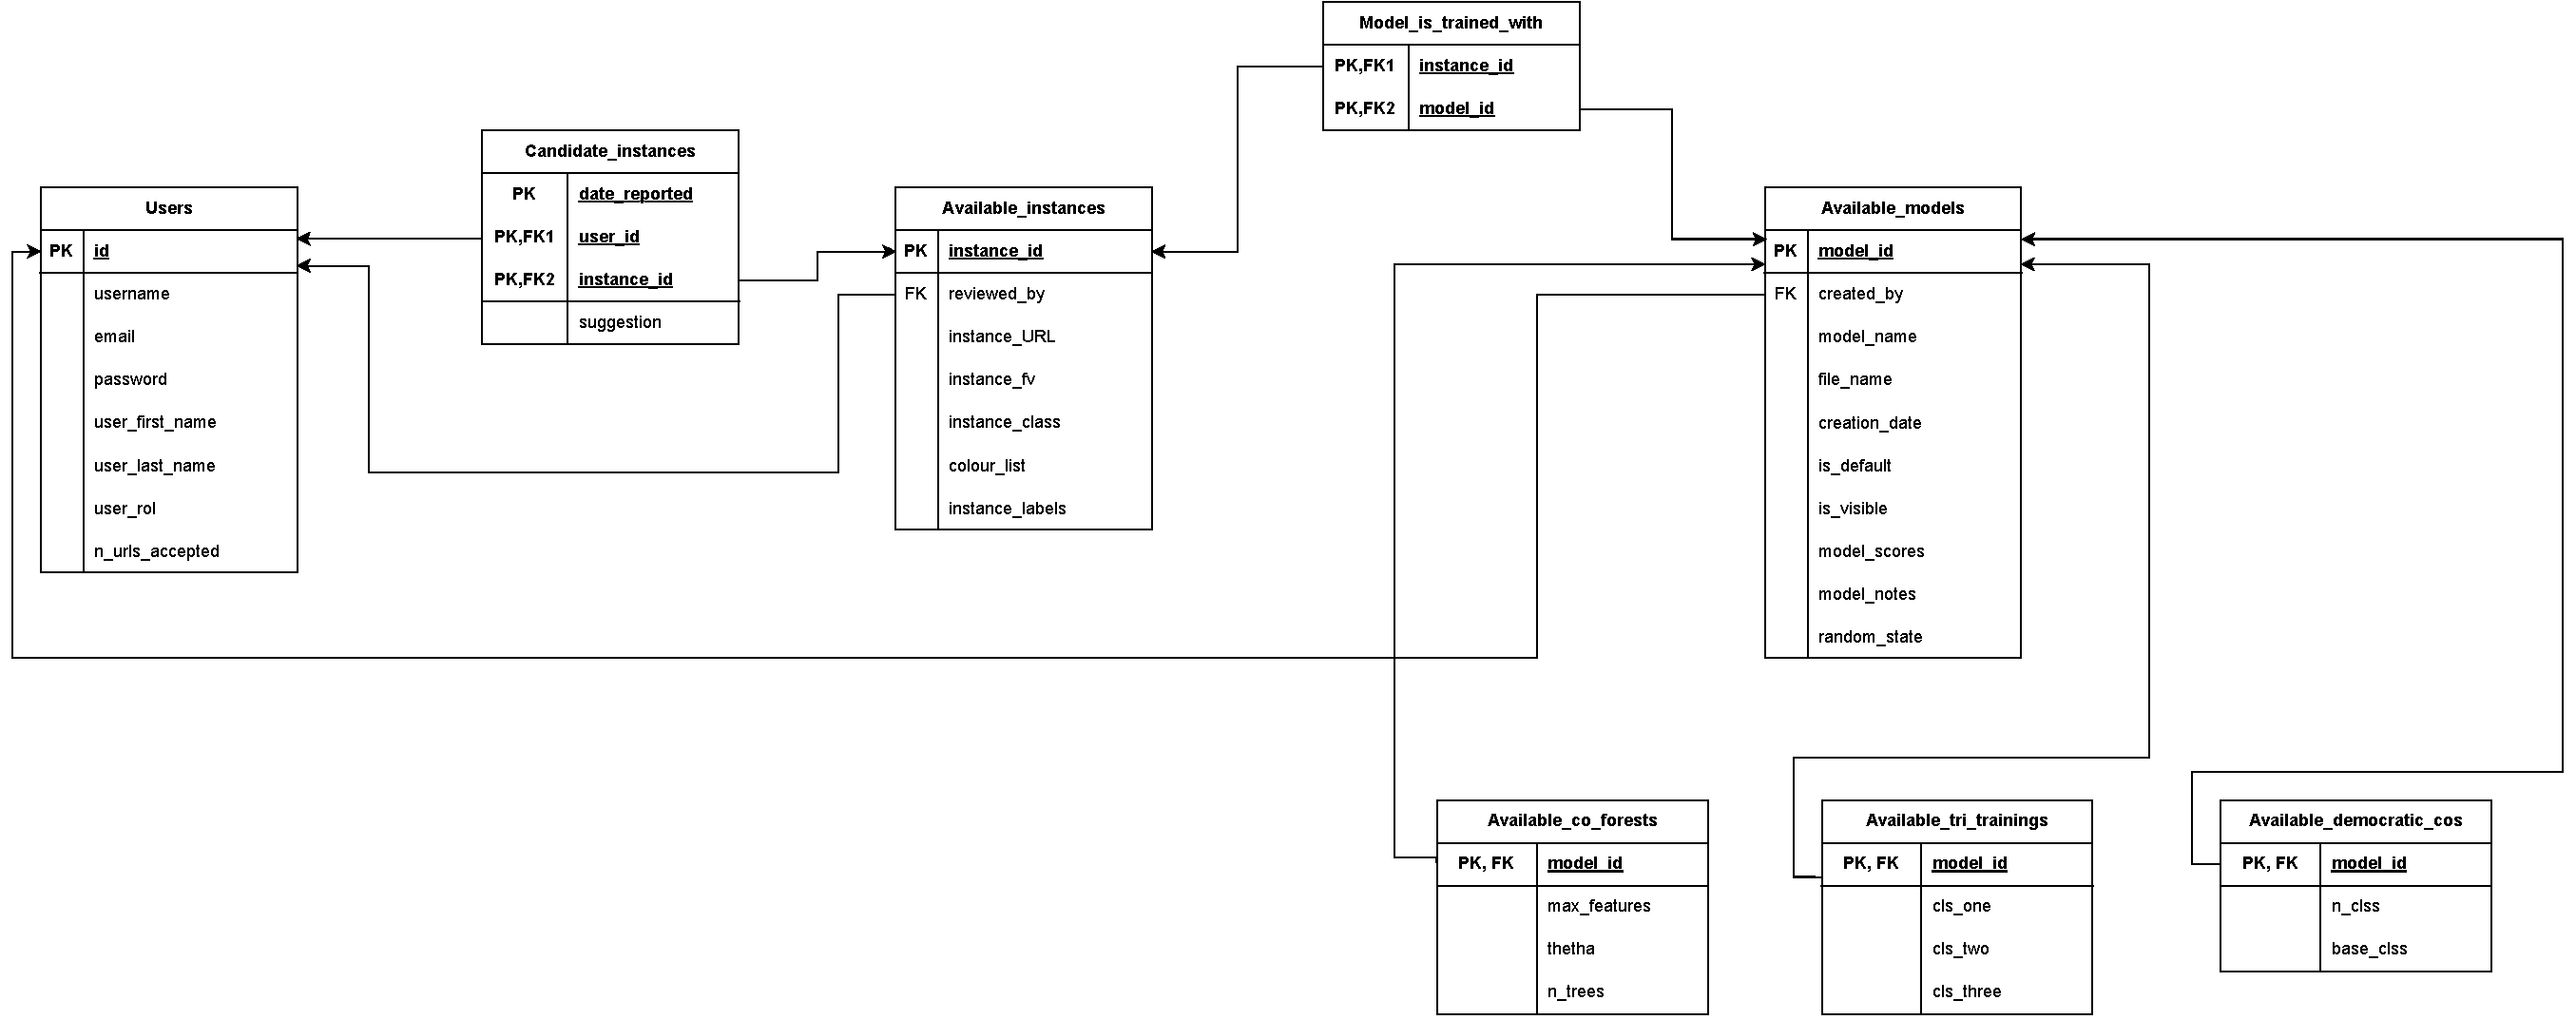
\includegraphics[scale=0.46]{../img/anexos/diagrams/relational}
		\label{c:diagrama-relacional}
	\end{figure}
\end{landscape}

\subsection{Diccionario de datos}

Se adjunta a continuación, para cada tabla, el diccionario de datos correspondiente. \label{c:diccionario_datos}

\subsubsection{Tabla de usuarios (\texttt{Users})}

\begin{table}
	\scalebox{0.80}{
		\begin{tabular}{@{}p{5em} p{6em} p{6em} p{20em}@{}}
			\toprule
			\textbf{Nombre} & \textbf{Tipo} & \textbf{Columna} & \textbf{Descripción}\\
			\midrule
			\texttt{\textbf{\underline{id}}} & \texttt{INTEGER} & \texttt{\textbf{\underline{PK}}} & Identificador. Generado automáticamente mediante una secuencia. \\
			\texttt{username} &  \texttt{VARCHAR(64)} & \texttt{UNIQUE NOT NULL} & Inmutable. Nombre de usuario proporcionado en el registro.\\
			\texttt{email} & \texttt{VARCHAR(128)} & \texttt{UNIQUE NOT NULL} & Inmutable. Email del usuario proporcionado en el registro.\\
			\texttt{password} &  \texttt{BYTEA} & \texttt{NOT NULL} & Contraseña cifrada mediante \texttt{sha-512}. La \textit{salt} se obtiene aleatoriamente y está cifrada en \texttt{sha-256}.\\
			\texttt{user\_first \_name} & \texttt{VARCHAR(64)} & & Nombre del usuario.\\
			\texttt{user\_last \_name} & \texttt{VARCHAR(64)} & & Apellidos del usuario. \\
			\texttt{user\_rol} & \texttt{VARCHAR(16)} & \texttt{NOT NULL} & Rol del usuario. Puede ser <<standard>> o <<admin>>. Por defecto: <<standard>>. \\
			\texttt{n\_urls \_accepted} & \texttt{INTEGER} &  &  Atributo de usuarios <<standard>>. Contador de aquellas instancias que han sido reportadas y aceptadas por un administrador. \\
			\bottomrule
		\end{tabular}
	}
	\caption[Diccionario de datos: \texttt{Users}]{Diccionario de datos. Tabla correspondiente a la clase \texttt{Users}.}
	\label{datadic:users}
\end{table}

La tabla~\ref{datadic:users} almacena la información relevante de cada usuario registrado en la base de datos. Si se comprueba el diagrama E-R, se puede comprobar que una peculiaridad de esta tabla es que es una ISA. Debido a que, además del discriminante (usuario administrador o estándar), únicamente hay un atributo que diferencia ambas clases, se ha decidido implementar utilizando una sola tabla. Cabe destacar que la contraseña está correctamente cifrada mediante \texttt{sha-512} y la sal\footnote{\textit{Salt} es un término que se refiere a bits aleatorios usados como entrada (junto a la contraseña) en una función derivadora de claves (cuya salida es la contraseña cifrada).} se ha cifrado en \texttt{sha-256}.


\subsubsection{Tabla de instancias (\texttt{Available\_instances})}

\begin{table}
	\scalebox{0.80}{
	\begin{tabular}{@{}p{6em} p{6em} p{5em} p{20em}@{}}
		\toprule
		\textbf{Nombre} & \textbf{Tipo} & \textbf{Columna} & \textbf{Descripción}\\
		\midrule
			\texttt{\textbf{\underline{instance\_id}}} & \texttt{INTEGER} & \texttt{\textbf{\underline{PK}}} & Identificador. Generado automáticamente mediante una secuencia. \\
			\texttt{reviewed\_by} & \texttt{INTEGER} & \texttt{FK(Users)} & En caso de estar vacío, significa que la URL todavía no ha sido aprobada por un administrador y está en proceso de revisión, por lo que no se puede utilizar para entrenar modelos.\\
			\texttt{instance\_url} & \texttt{VARCHAR(256)} & \texttt{UNIQUE NOT NULL} &  URL de la instancia. Inmutable.\\
			\texttt{instance\_fv} &  \texttt{INTEGER ARRAY[19]} & & Vector de características de la URL.   \\
			\texttt{instance \_class} & \texttt{INTEGER} & & Etiqueta de la clase. Puede valer $0$ si la URL es legítima o $1$ en caso de que sea \textit{phishing}. \\
			\texttt{colour\_list} & \texttt{VARCHAR(16)} & & Puede ser <<black-list>>, <<white-list>> o estar vacío. En caso de contener un valor ha de ser aprobada por un administrador. \\
			\texttt{instance \_labels} & \texttt{VARCHAR(64) ARRAY[]} & &  Se preve que el campo varíe bastante, por lo que el tipo de dato no se ha definido como \texttt{VARCHAR}. Contiene etiquetas relacionadas con la instancia.\\
			\bottomrule
		\end{tabular}
	}
	\caption[Diccionario de datos: \texttt{Available\_instances}]{Diccionario de datos. Tabla correspondiente a la clase \texttt{Available\_instances}.}
	\label{datadic:instances}
\end{table}

La tabla~\ref{datadic:instances} almacena la información asociada a cada instancia disponible en el \textit{dataset}. Las instancias son URLs que pueden ser utilizadas posteriormente para entrenar y probar modelos. Además, esta tabla también almacena enlaces reportados por usuarios por pertenecer a una lista blanca o negra.

\subsubsection{Tabla de modelos (\texttt{Available\_models})}

La tabla~\ref{datadic:models} almacena los modelos de aprendizaje que han sido creados por un administrador y están disponibles en la \textit{web} para su uso.

\begin{table}
	\scalebox{0.80}{
	\begin{tabular}{@{}p{6em} p{6em} p{5em} p{20em}@{}}
		\toprule
		\textbf{Nombre} & \textbf{Tipo} & \textbf{Columna} & \textbf{Descripción}\\
		\midrule
			\texttt{\textbf{\underline{model\_id}}} & \texttt{INTEGER} & \texttt{\textbf{\underline{PK}}} & Identificador. Generado automáticamente mediante una secuencia. \\
			\texttt{created\_by} & \texttt{INTEGER} & \texttt{FK(Users) NOT NULL ON DELETE CASCADE} &  Enlace al administrador que ha creado un determinado modelo. Dependencia por existencia.\\
			\texttt{model\_name} & \texttt{VARCHAR(64)} & \texttt{UNIQUE NOT NULL} & Inmutable. Nombre común y visible para los usuarios. \\
			\texttt{file\_name} & \texttt{VARCHAR(64)} & \texttt{UNIQUE NOT NULL} & Inmutable. Preferiblemente seguirá la sintáxis \texttt{nombre\_v-a-b-c.pkl}, donde $a$, $b$, $c$ son los números de versión (ejemplo: \texttt{cof\_v-1-0-0.pkl})    \\
			\texttt{creation \_date} & \texttt{TIMESTAMP} & &  Fecha de creación.   \\
			\texttt{is\_default} & \texttt{BOOLEAN} & \texttt{NOT NULL} & Por defecto <<false>>. Determina si un clasificador es el utilizado por defecto (cuando un usuario realiza una consulta y no selecciona ningún modelo).   \\
			\texttt{is\_visible} & \texttt{BOOLEAN} & \texttt{NOT NULL} & Por defecto <<true>>. Determina si un clasificador está visible en la \textit{web} y disponible para ser utilizado.\\
			\texttt{model\_scores} & \texttt{FLOAT ARRAY[5]} & \texttt{NOT NULL} & Por defecto \texttt{[0.0, 0.0, 0.0, 0.0, 0.0]}. Son las últimas estadísticas del último \textit{test} realizado al clasificador. Las columnas (en este orden) corresponden a las métricas \textit{accuracy}, \textit{precision}, \textit{recall}, F1 y AUC. \\			
			\texttt{model\_ algorithm} & \texttt{VARCHAR(2)} & \texttt{NOT NULL} & Discriminante. Tomará valores entre \texttt{dc}, \texttt{tt} o \texttt{cf} controlados por aplicación.\\
			\texttt{model\_notes} & \texttt{VARCHAR(512)} & & Notas acerca del \textit{ensemble}.\\
			\texttt{random\_state} & \texttt{INTEGER} & & Semilla aleatoria.  \\
			\bottomrule
		\end{tabular}
	}
	\caption[Diccionario de datos: \texttt{Available\_models}]{Diccionario de datos: tabla correspondiente a la clase \texttt{Available\_models}.}
	\label{datadic:models}
\end{table}

Si se comprueba el diagrama E-R, se puede comprobar que esta tabla es una ISA. En este caso se ha decidido implementar considerando que es una interrelación 1:1. Por ello, se ha creado una tabla para la generalización y otra tabla para cada una de las especializaciones. Estas se enumeran a continuación:

\begin{itemize}
	\item \textbf{\texttt{Available\_co\_forests}}: los modelos pertenecientes a este algoritmo poseen los atributos de la tabla~\ref{datadic:coforest}.

	\begin{table}
	\scalebox{0.80}{
	\begin{tabular}{@{}p{6em} p{5em} p{6em} p{20em}@{}}
		\toprule
		\textbf{Nombre} & \textbf{Tipo} & \textbf{Columna} & \textbf{Descripción}\\
		\midrule
				\texttt{\textbf{\underline{model\_id}}} & \texttt{INTEGER} & \texttt{\textbf{\underline{PK}}, FK(Available \_models) ON DELETE CASCADE} & Identificador. Generado por la secuencia de la tabla padre e introducido mediante código (debe coincidir). \\
				\texttt{max\_features} & \texttt{VARCHAR(8)} & \texttt{NOT NULL} & Parámetro del árbol de decisión. Puede ser <<sqrt>> o <<log2>>. Por defecto <<log2>>.   \\
				\texttt{thetha} & \texttt{FLOAT(3)} & \texttt{NOT NULL} & Parámetro thetha del \textit{ensemble} (umbral de confianza). Por defecto 0.75.   \\
				\texttt{n\_trees} & \texttt{INTEGER} & \texttt{NOT NULL} & Número de árboles. Por defecto 3.   \\
				\bottomrule
			\end{tabular}
		}
		\caption[Diccionario de datos: \texttt{Available\_co\_forests}]{Diccionario de datos: tabla correspondiente a la clase \texttt{Available\_co\_forests}.}
		\label{datadic:coforest}
	\end{table}

	\item \textbf{\texttt{Available\_tri\_trainings}}: los modelos pertenecientes a este algoritmo poseen los atributos de la tabla~\ref{datadic:tritraining}.

	\begin{table}
	\scalebox{0.80}{
	\begin{tabular}{@{}p{6em} p{5em} p{6em} p{20em}@{}}		
		\toprule
		\textbf{Nombre} & \textbf{Tipo} & \textbf{Columna} & \textbf{Descripción}\\
		\midrule
				\texttt{\textbf{\underline{model\_id}}} & \texttt{INTEGER} & \texttt{\textbf{\underline{PK}}, FK(Available \_models) ON DELETE CASCADE} & Identificador. Generado por la secuencia de la tabla padre e introducido mediante código (debe coincidir).\\
				\texttt{cls\_one} & \texttt{VARCHAR(4)} & \texttt{NOT NULL}  &  Algoritmo del primer estimador base. Puede ser <<kNN>>, <<NB>> o <<DT>>.\\
				\texttt{cls\_two} & \texttt{VARCHAR(4)} & \texttt{NOT NULL} & Algoritmo del segundo estimador base. Puede ser <<kNN>>, <<NB>> o <<DT>>.\\
				\texttt{cls\_three} & \texttt{VARCHAR(4)} & \texttt{NOT NULL} & Algoritmo del tercer estimador base. Puede ser <<kNN>>, <<NB>> o <<DT>>.\\
				\bottomrule
			\end{tabular}
		}
		\caption[Diccionario de datos: \texttt{Available\_tri\_trainings}]{Diccionario de datos: tabla correspondiente a la clase \texttt{Available\_tri\_trainings}.}
		\label{datadic:tritraining}
	\end{table}

	\item \textbf{\texttt{Available\_democratic\_cos}}: los modelos pertenecientes a este algoritmo poseen los atributos de la tabla~\ref{datadic:democraticco}.

	\begin{table}
	\scalebox{0.80}{
	\begin{tabular}{@{}p{6em} p{5em} p{6em} p{20em}@{}}		
		\toprule
		\textbf{Nombre} & \textbf{Tipo} & \textbf{Columna} & \textbf{Descripción}\\
		\midrule
				\texttt{\textbf{\underline{model\_id}}} & \texttt{INTEGER} & \texttt{\textbf{\underline{PK}}, FK(Available \_models) ON DELETE CASCADE} & Identificador. Generado por la secuencia de la tabla padre e introducido mediante código (debe coincidir).\\
				\texttt{n\_clss} & \texttt{INTEGER} & \texttt{NOT NULL} & Número de clasificadores base.\\
				\texttt{base\_clss} & \texttt{VARCHAR(4) ARRAY} & \texttt{NOT NULL}  & Array con los algoritmos pertenecientes a los estimadores base. Los valores que puede contener son <<kNN>>, <<NB>> o <<DT>>.\\
				\bottomrule
			\end{tabular}
		}
		\caption[Diccionario de datos: \texttt{Available\_democratic\_cos}]{Diccionario de datos: tabla correspondiente a la clase \texttt{Available\_democratic\_cos}.}
		\label{datadic:democraticco}
	\end{table}
\end{itemize}

\subsubsection{Tablas de relación}

Se enumeran a continuación las tablas que son resultado de una relación entre entidades.

\begin{itemize}
	\item \textbf{\texttt{Candidate\_instances}}: en la tabla~\ref{datadic:candidate_instances} se almacenan aquellas instancias que han sido reportadas por un usuario y necesitan ser revisadas por un administrador antes de poder ser utilizadas para entrenar o probar modelos. Como se puede comprobar, se trata de una relación ternaria entre el usuario, la instancia reportada y la fecha (puede ser que un usuario reporte la misma URL más de una vez en dos fechas distintas). Es destacable que este es uno de los casos (excepción) en los que no merece la pena que la entidad <<Fecha>> pase a ser tabla debido a que no posee ninguna característica relevante.
	
		\begin{table}
		\scalebox{0.80}{
		\begin{tabular}{@{}p{7em} p{6em} p{7em} p{17em}@{}}		
			\toprule
			\textbf{Nombre} & \textbf{Tipo} & \textbf{Columna} & \textbf{Descripción}\\
			\midrule
				\texttt{user\_id} & \texttt{INTEGER} & \texttt{FK(Users) ON DELETE CASCADE} & Identificador del usuario que ha reportado la URL. \\
				\texttt{instance\_id} & \texttt{INTEGER} & \texttt{FK(Available \_instances) ON DELETE CASCADE} & Identificador de la URL reportada. \\
				\texttt{date\_reported} & \texttt{TIMESTAMP} & & Fecha de envío del formulario.     \\
				\texttt{suggestion} & \texttt{VARCHAR(16)} & \texttt{NOT NULL} & Lo que el usuario denuncia que la URL es (ejemplo: <<white-list>>).   \\\\
				\multicolumn{3}{l}{\hfill \texttt{\textbf{\underline{PK(user\_id, instance\_id, date\_reported)}}}} & Clave primaria compuesta de la relación. \\
				\bottomrule
			\end{tabular}
		}
		\caption[Diccionario de datos: \texttt{Candidate\_instances}]{Diccionario de datos: tabla correspondiente a la clase \texttt{Candidate\_instances}.}
		\label{datadic:candidate_instances}
		\end{table}

	\item \textbf{\texttt{Model\_is\_trained\_with}}: en la tabla~\ref{datadic:modeltrainedwith} se almacena qué instancia ha sido utilizada para entrenar qué modelo en el sistema.
	
		\begin{table}
		\scalebox{0.80}{
		\begin{tabular}{@{}p{7em} p{6em} p{7em} p{17em}@{}}		
			\toprule
			\textbf{Nombre} & \textbf{Tipo} & \textbf{Columna} & \textbf{Descripción}\\
			\midrule
				\texttt{model\_id} & \texttt{INTEGER} & \texttt{FK(Available \_models) ON DELETE CASCADE} & Identificador del modelo que ha sido entrenado. \\
				\texttt{instance\_id} & \texttt{INTEGER} & \texttt{FK(Available \_instances) ON DELETE CASCADE} & Identificador de la instancia utilizada en la fase de entrenamiento. \\\\
				\multicolumn{3}{l}{\hfill \texttt{\textbf{\underline{PK(model\_id, instance\_id)}}}} & Clave primaria compuesta de la relación. \\
				\bottomrule
			\end{tabular}
		}
		\caption[Diccionario de datos: \texttt{Model\_is\_trained\_with}]{Diccionario de datos: tabla correspondiente a la clase \texttt{Model\_is\_trained\_with}.}
		\label{datadic:modeltrainedwith}
	\end{table}
\end{itemize}


\section{Diseño procedimental}
\label{s:diseño-procedimental}

En el desarrollo de \textit{software}, el diseño procedimental se refiere a la definición de pasos ordenados para realizar una determinada funcionalidad. Se utiliza para crear métodos y se basa en la descomposición del problema en pequeñas tareas ejecutadas secuencialmente para alcanzar el resultado deseado. Para ello, se ha hecho uso de diagramas de secuencia UML\footnote{El Lenguaje Unificado de Modelado (UML) es un lenguaje estándar de modelado visual utilizado durante el diseño y la implementación de sistemas de \textit{software}.}. Estos muestran la interacción entre distintos componentes en un sistema.

Con el fin de facilitar la comprensión de ciertos métodos, se muestran a continuación los diagramas de algunas de las principales funcionalidades implementadas.



\noindent
\framebox{\parbox{\dimexpr\linewidth-2\fboxsep-2\fboxrule}{\vspace*{5px} \textbf{Importante:} es destacable que, debido a las peculiaridades de la aplicación, en ciertas ocasiones se ha hecho una interpretación libre de los diagramas UML incorporando los principios semánticos de este lenguaje. Un ejemplo son las funciones correspondientes a la aplicación de Flask, que se han incorporado en los diagramas (sin negrita ni subrayado) debido a que manejan la lógica de negocio, pero no son objetos al uso.\vspace*{5px}}}

\begin{itemize}
	\item \textbf{Página principal}: en el diagrama~\ref{c:diagrama-seq-index} se representan los pasos seguidos para la acción más común: analizar una URL. Como se puede comprobar, el usuario realiza una petición y permanece esperando en la pantalla de carga correspondiente. Mientras tanto, el analizador procesa su petición.
	
	Para extraer el vector de características es necesario que la dirección introducida sea alcanzable. En caso de que no lo sea, se realizan correcciones (completar protocolos, corregir sintaxis, etc.). Posteriormente se intenta recuperar posible información existente en la base de datos acerca de dicha instancia (si pertenece a una lista blanca o negra, si ya se tiene almacenado su vector de características, etc.).
	
	Si la dirección no es alcanzable y no hay información previa, se devuelve al usuario un mensaje informativo (es una excepción, no se puede analizar ni mostrar nada).
	
	En el caso de que exista información previa acerca de dicha instancia (el vector de características está almacenado), se puede analizar (ya sea llamable o no). Este camino también es seguido en caso de que el usuario seleccione el <<análisis rápido>>, ya que recuperar el vector de características de la base de datos no es temporalmente costoso.
	
	Por último, en caso de que la URL sea llamable y si no se ha recorrido ningún camino previo, se analiza utilizando el método de extracción de vector de características expuesto en la sección teórica de la memoria. Este proceso requiere unos 40 segundos aproximadamente, aunque varía en función de las características de cada página (número de enlaces que contenga, etc.).
	
	Si no ha ocurrido ninguna excepción, en cualquiera de las opciones se ha extraído el vecto de características. Por lo tanto, sólo queda analizar y mostrar los resultados haciendo uso de técnicas visuales (gráficos interactivos) en el \textit{dashboard}, por lo que se redirige a esta pantalla. En caso de que ocurra alguna excepción, el usuario será redirigido a la página principal con un mensaje informativo.

	\begin{figure}[h]
		\caption[Diagrama: secuencia (reportar url)]{Diagrama de secuencia de la página para reportar una URL.}
		\centering
		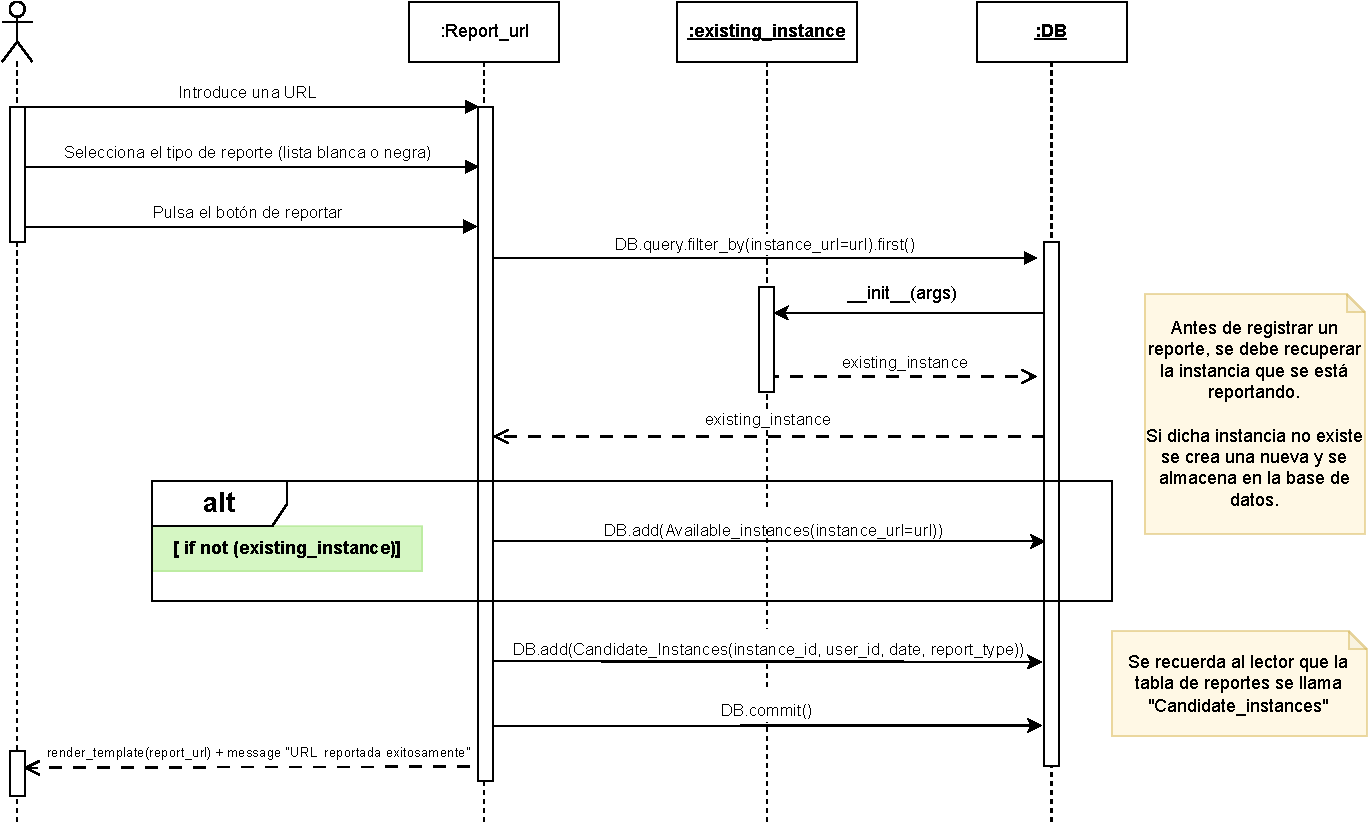
\includegraphics[width=\textwidth]{../img/anexos/diagrams/sequence-report_url}
		\label{c:diagrama-seq-report_url}
	\end{figure}

	\item \textbf{Página para reportar una URL}: la secuencia se ilustra en el diagrama~\ref{c:diagrama-seq-report_url}. Como se puede comprobar, el usuario tan solo ha de introducir la URL, seleccionar el tipo (lista blanca o lista negra) y aceptar.
	
	Como internamente la tabla donde se almacenan las URLs reportadas necesita información para incluir un nuevo registro (identificador de la instancia y del usuario), se intenta recuperar la instancia que se está reportando. En caso de no existir, se crea una nueva y se añade a la base de datos. Por último, se incluye el reporte con los datos y se redirige al usuario a la misma página con un mensaje informativo.
	
	Es destacable que un usuario registrado no va a poder acceder a esta pantalla (antes será redirigido por el sistema de control a la página de inicio de sesión).

	\item \textbf{Nueva instancia}: en el diagrama~\ref{c:diagrama-seq-instan} se muestra los pasos necesarios para crear una nueva instancia (es decir, una URL con su vector de características).
	
	En primer lugar, el usuario ineractúa con un formulario y, cuando confirma la selección, espera en una pantalla de carga al resultado. Internamente se comprueba que la instancia no exista ya en la base de datos (no hay ningún beneficio en almacenar URLs duplicadas) y, en caso de que no lo haga, se crea una con los datos introducidos por el usuario, además de las etiquetas por defecto.
	
	Es destacable que, debido a que generar un vector de características requiere tiempo y que la página esté activa, se ha permitido añadir instancias sin este campo (para que se genere más adelante). Aún así se debe recordar que una instancia sin vector no puede ser utilizada para entrenar modelos, pero sí se puede saber su pertenencia a una lista blanca o negra.
		
	\begin{figure}[h]
		\caption[Diagrama: secuencia (nueva instancia)]{Diagrama de secuencia correspondiente a la creación de una nueva instancia.}
		\centering
		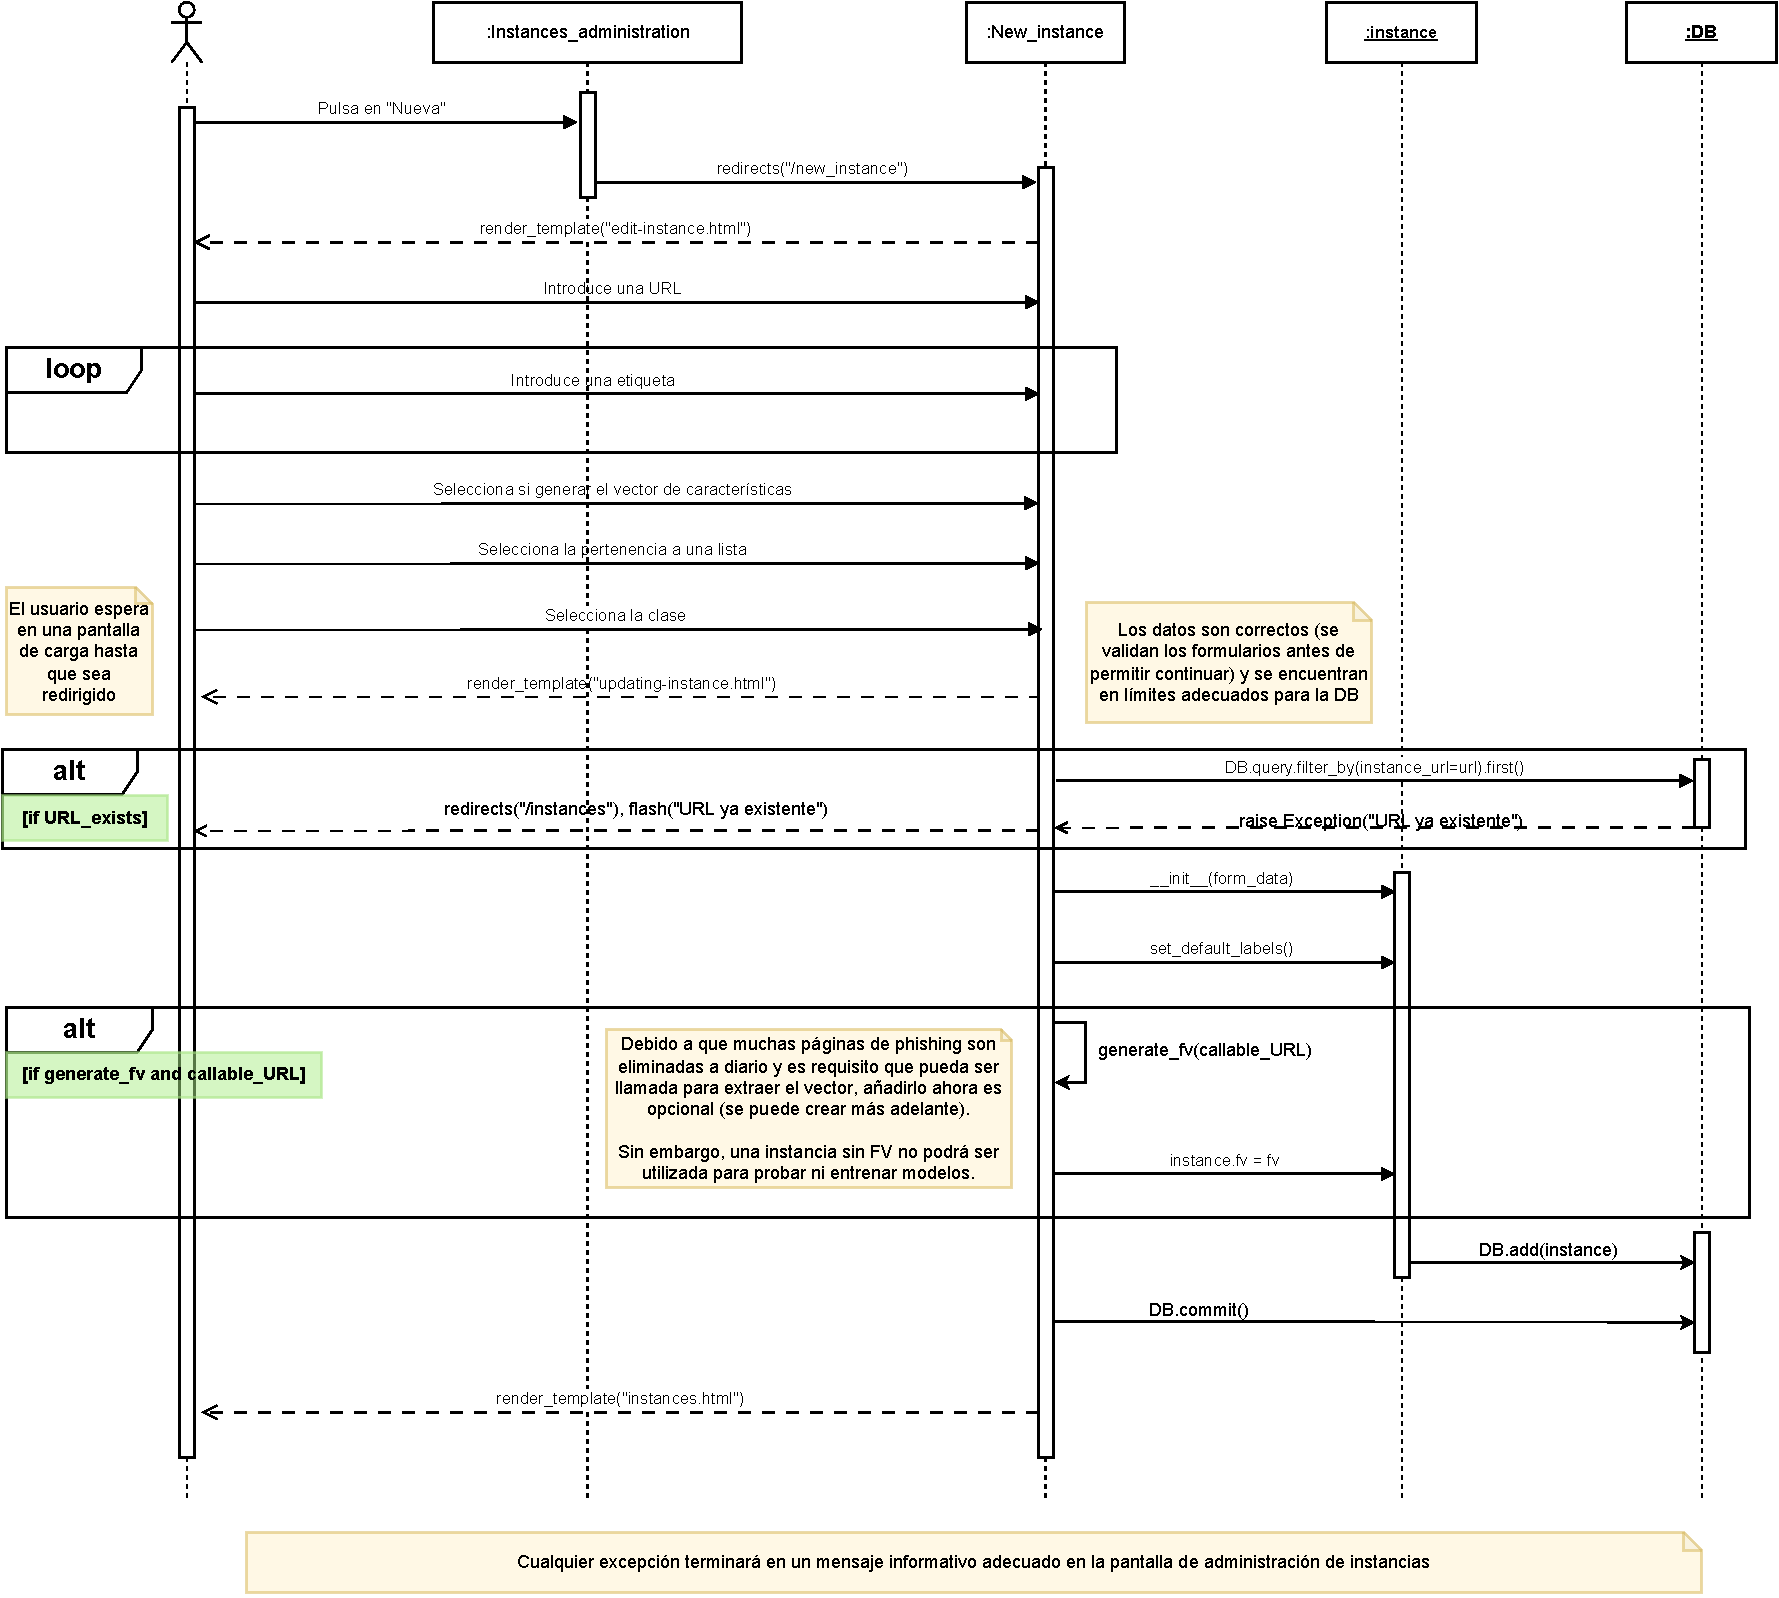
\includegraphics[width=\textwidth]{../img/anexos/diagrams/sequence-new_instance}
		\label{c:diagrama-seq-instan}
	\end{figure}

	\item \textbf{Evaluar modelo}: en el diagrama~\ref{c:diagrama-seq-test-model} se representa el flujo de comunicación correspondiente a la acción de evaluar modelos.
	
	Tras seleccionar un determinado modelo y pulsar en <<evaluar>>, el usuario deberá subir los datos (en formato correcto, si no será informado) o seleccionar si desea utilizar el \textit{dataset} de la aplicación. Internamente, la aplicación recupera el fichero asociado al modelo seleccionado y lo deserializa, consiguiendo un clasificador.
	
	Posteriormente se extrae el conjunto de \textit{test}. Si el usuario desea que se excluyan aquellas instancias vistas por el modelo durante el entrenamiento, la aplicación lo hará gracias a la tabla~\ref{datadic:modeltrainedwith} (\texttt{Model\_is\_trained \_with}). Por último, si el usuario lo desea, también se actualizarán las \textit{scores} del modelo y se mostrarán los resultados en una gráfica interactiva.
	
	\textbf{Importante}: En este diagrama es reseñable la diferencia entre el objeto \texttt{cls} y el objeto \texttt{model}. Mientras que uno es un objeto de Python (con sus métodos \texttt{fit} y \texttt{predict}), el otro es su equivalente en el modelo de datos. Es decir, el objeto que transporta los datos correspondientes al clasificador almacenados en la base de datos.
			
	\item \textbf{Aceptar sugerencia}: en el diagrama~\ref{c:diagrama-seq-accept-review} se muestra la comunicación que tiene lugar cuando un administrador acepta una sugerencia.
	
	En primer lugar, se recupera la instancia que se está reportando y se limpian las etiquetas asociadas a sugerencias. Posteriormente, se comprueba qué está denunciando el usuario y se modifica la instancia en consecuencia (por ejemplo, si el usuario denuncia que una URL pertenece a una lista blanca, se actualiza el campo de esa URL y se establece como tal). Por último, se elimina la sugerencia y se actualizan las etiquetas para eliminar posibles incoherencias.
	
	\textbf{Importante:} con el fin de simplificar el diagrama, se muestran a la derecha la clase \texttt{Available\_tags} y el objeto \texttt{report}. Estos se utilizan para realizar las comprobaciones que permiten analizar qué está denunciando el usuario para así modificar la instancia adecuadamente. Se puede observar que sus atributos son utilizados en la alternativa, pero no se ha dibujado el flujo con el fin de facilitar la visualización del diagrama.
	
	
	
\end{itemize}

	\begin{landscape}
		\begin{figure}[h]
			\caption[Diagrama: secuencia (página principal)]{Diagrama de secuencia de la página principal del analizador.}
			\centering
			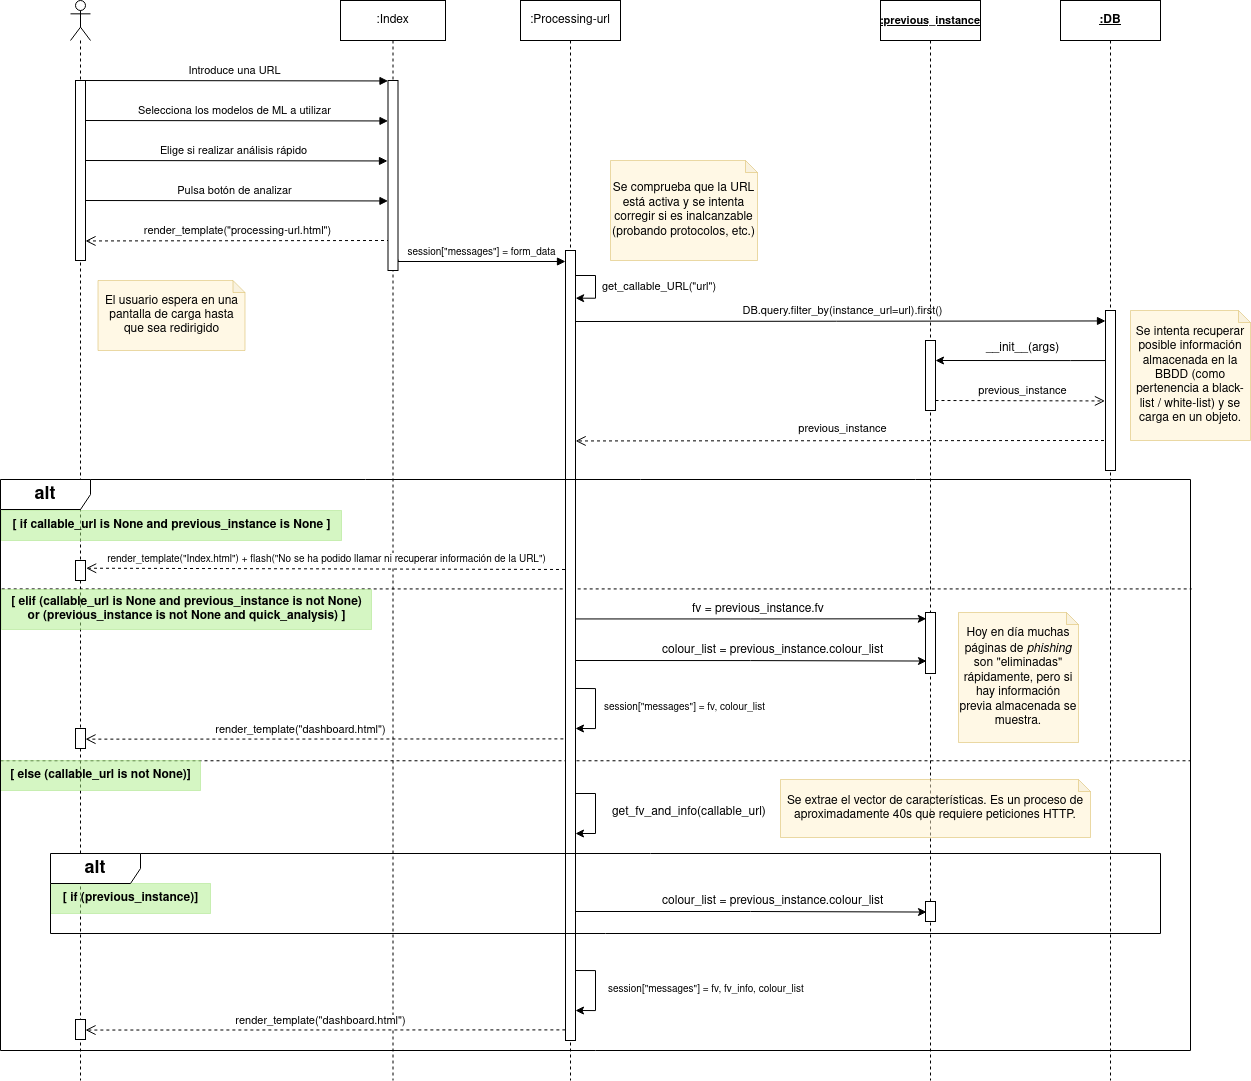
\includegraphics[scale=0.45]{../img/anexos/diagrams/sequence-index}
			\label{c:diagrama-seq-index}
		\end{figure}
	\end{landscape}

	\begin{landscape}
		\begin{figure}[h]
			\caption[Diagrama: secuencia (evaluar modelo)]{Diagrama de secuencia correspondiente a la evaluación de un modelo.}
			\centering
			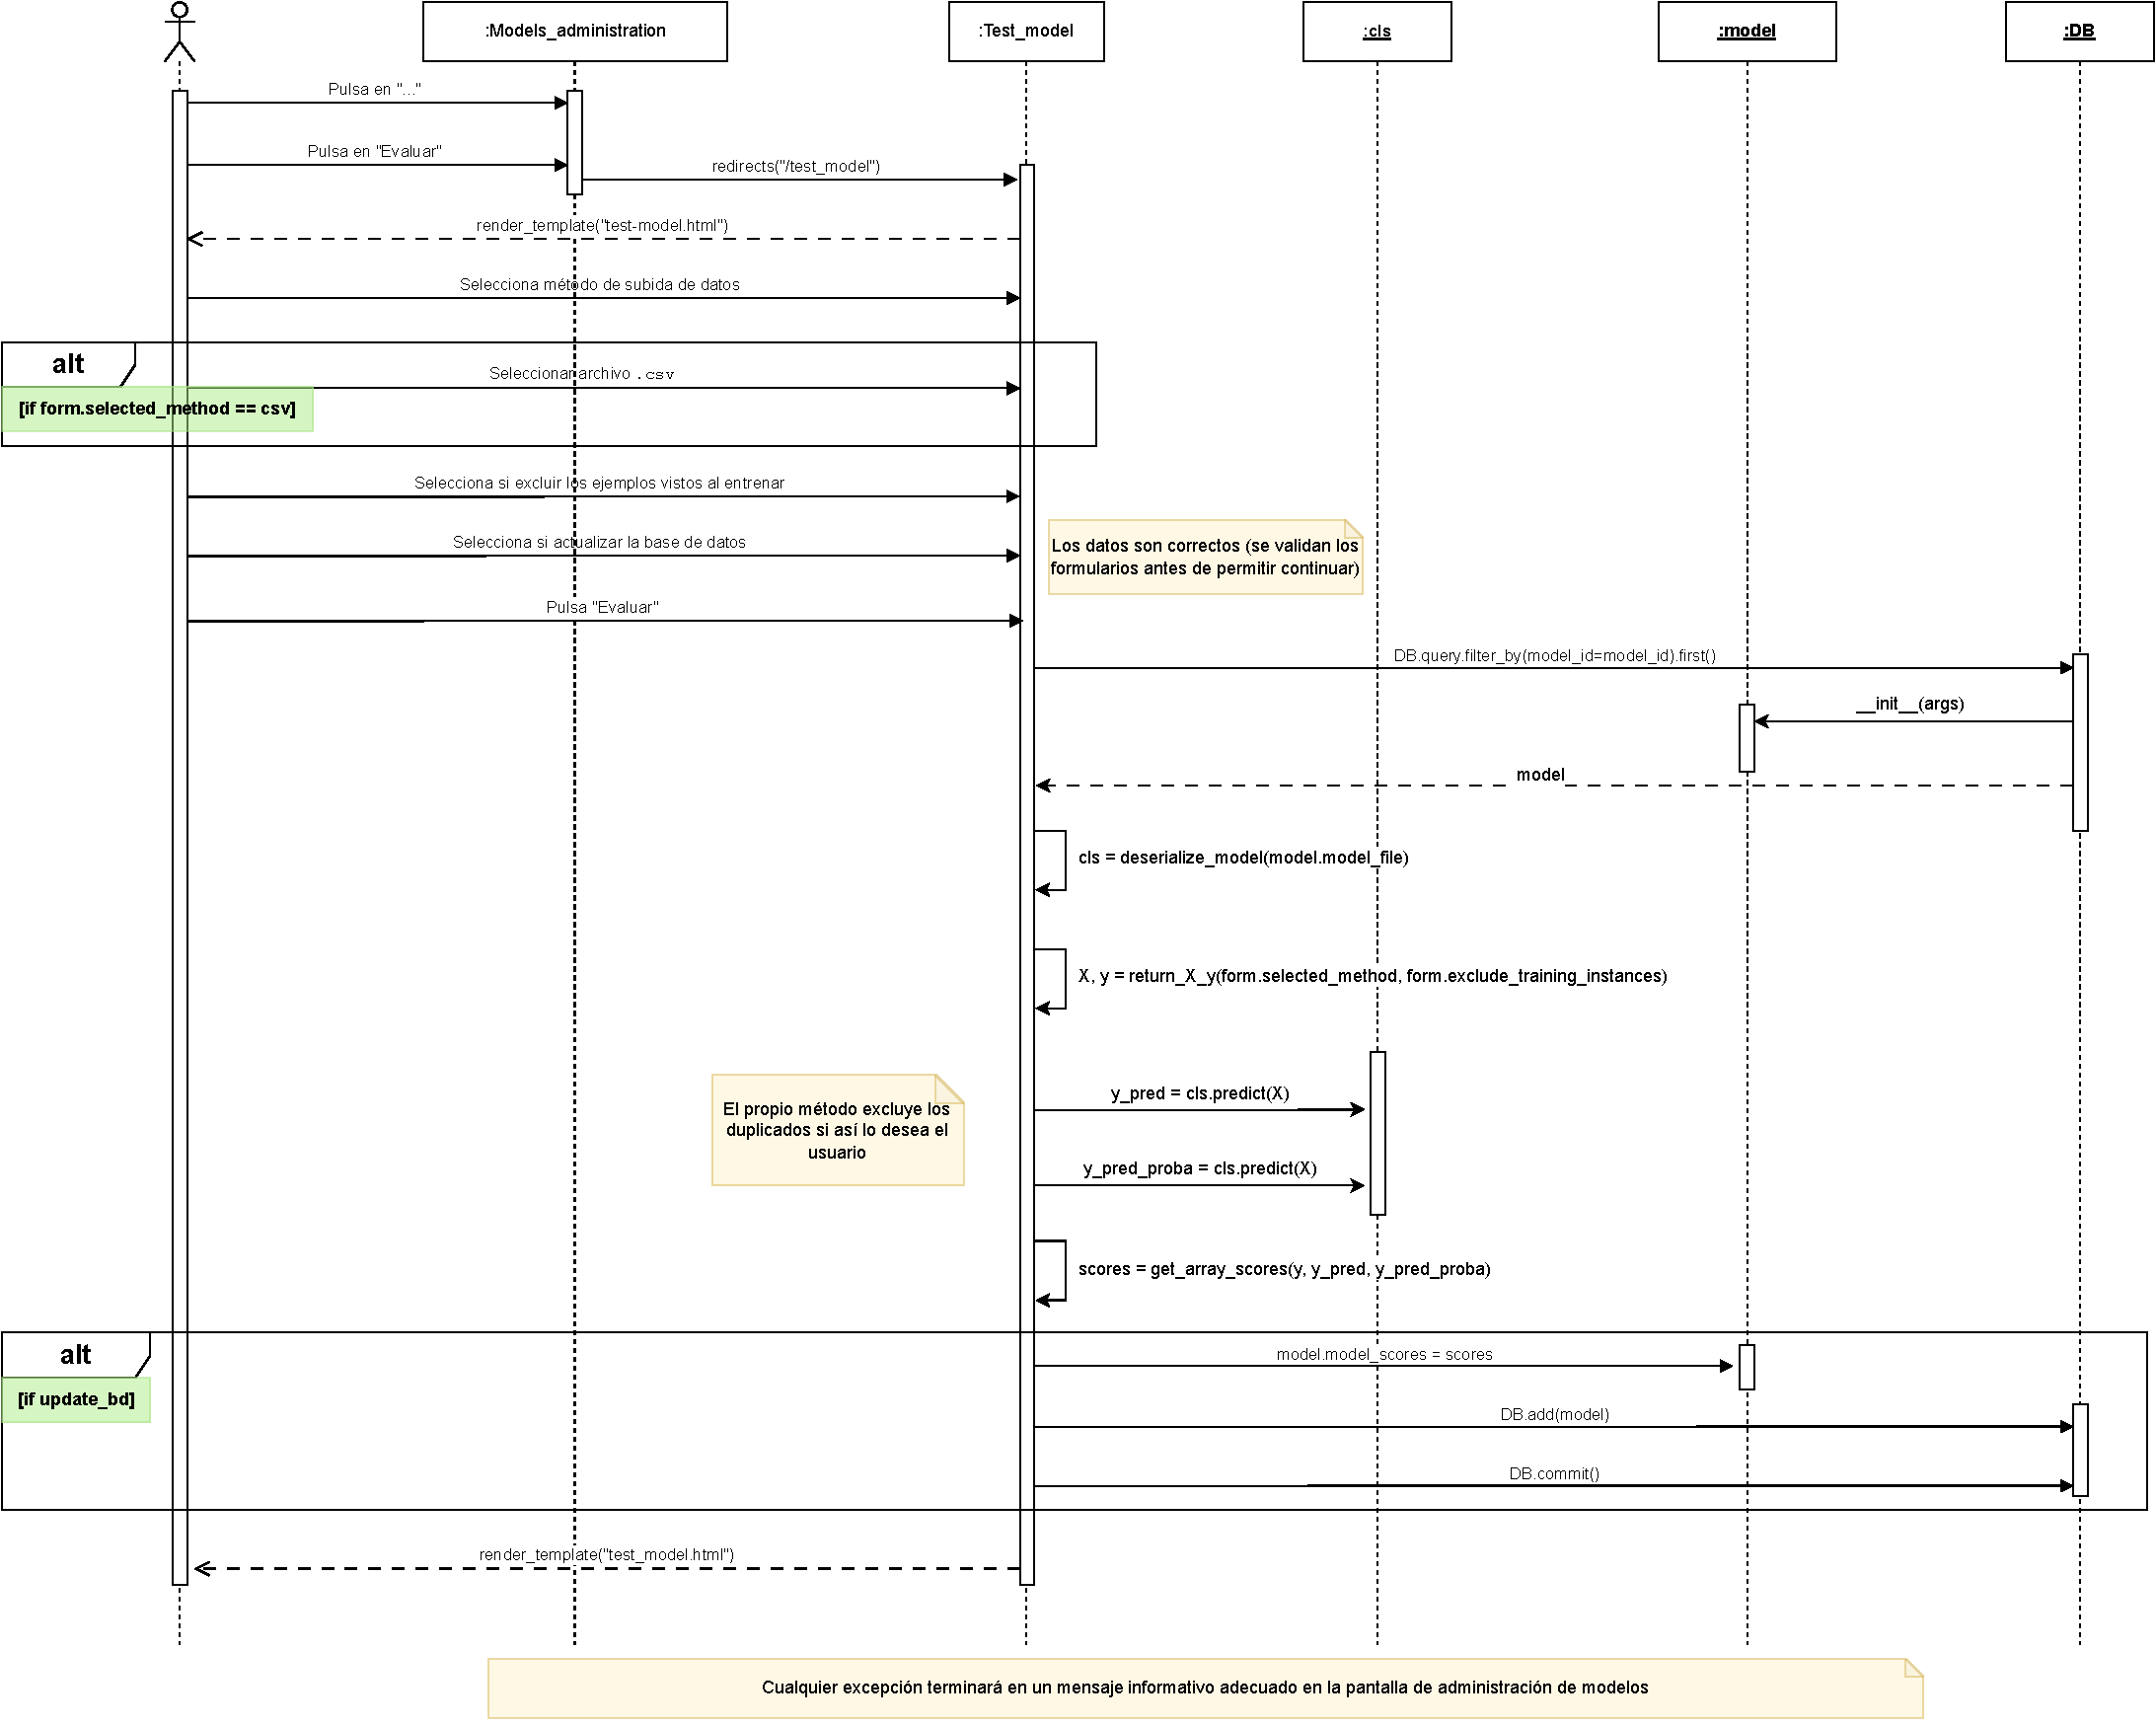
\includegraphics[scale=0.45]{../img/anexos/diagrams/sequence-test_model}
			\label{c:diagrama-seq-test-model}
		\end{figure}
	\end{landscape}

	\begin{landscape}
		\begin{figure}[h]
			\caption[Diagrama: secuencia (aceptar sugerencia)]{Diagrama de secuencia relativo a la aceptación de una sugerencia.}
			\centering
			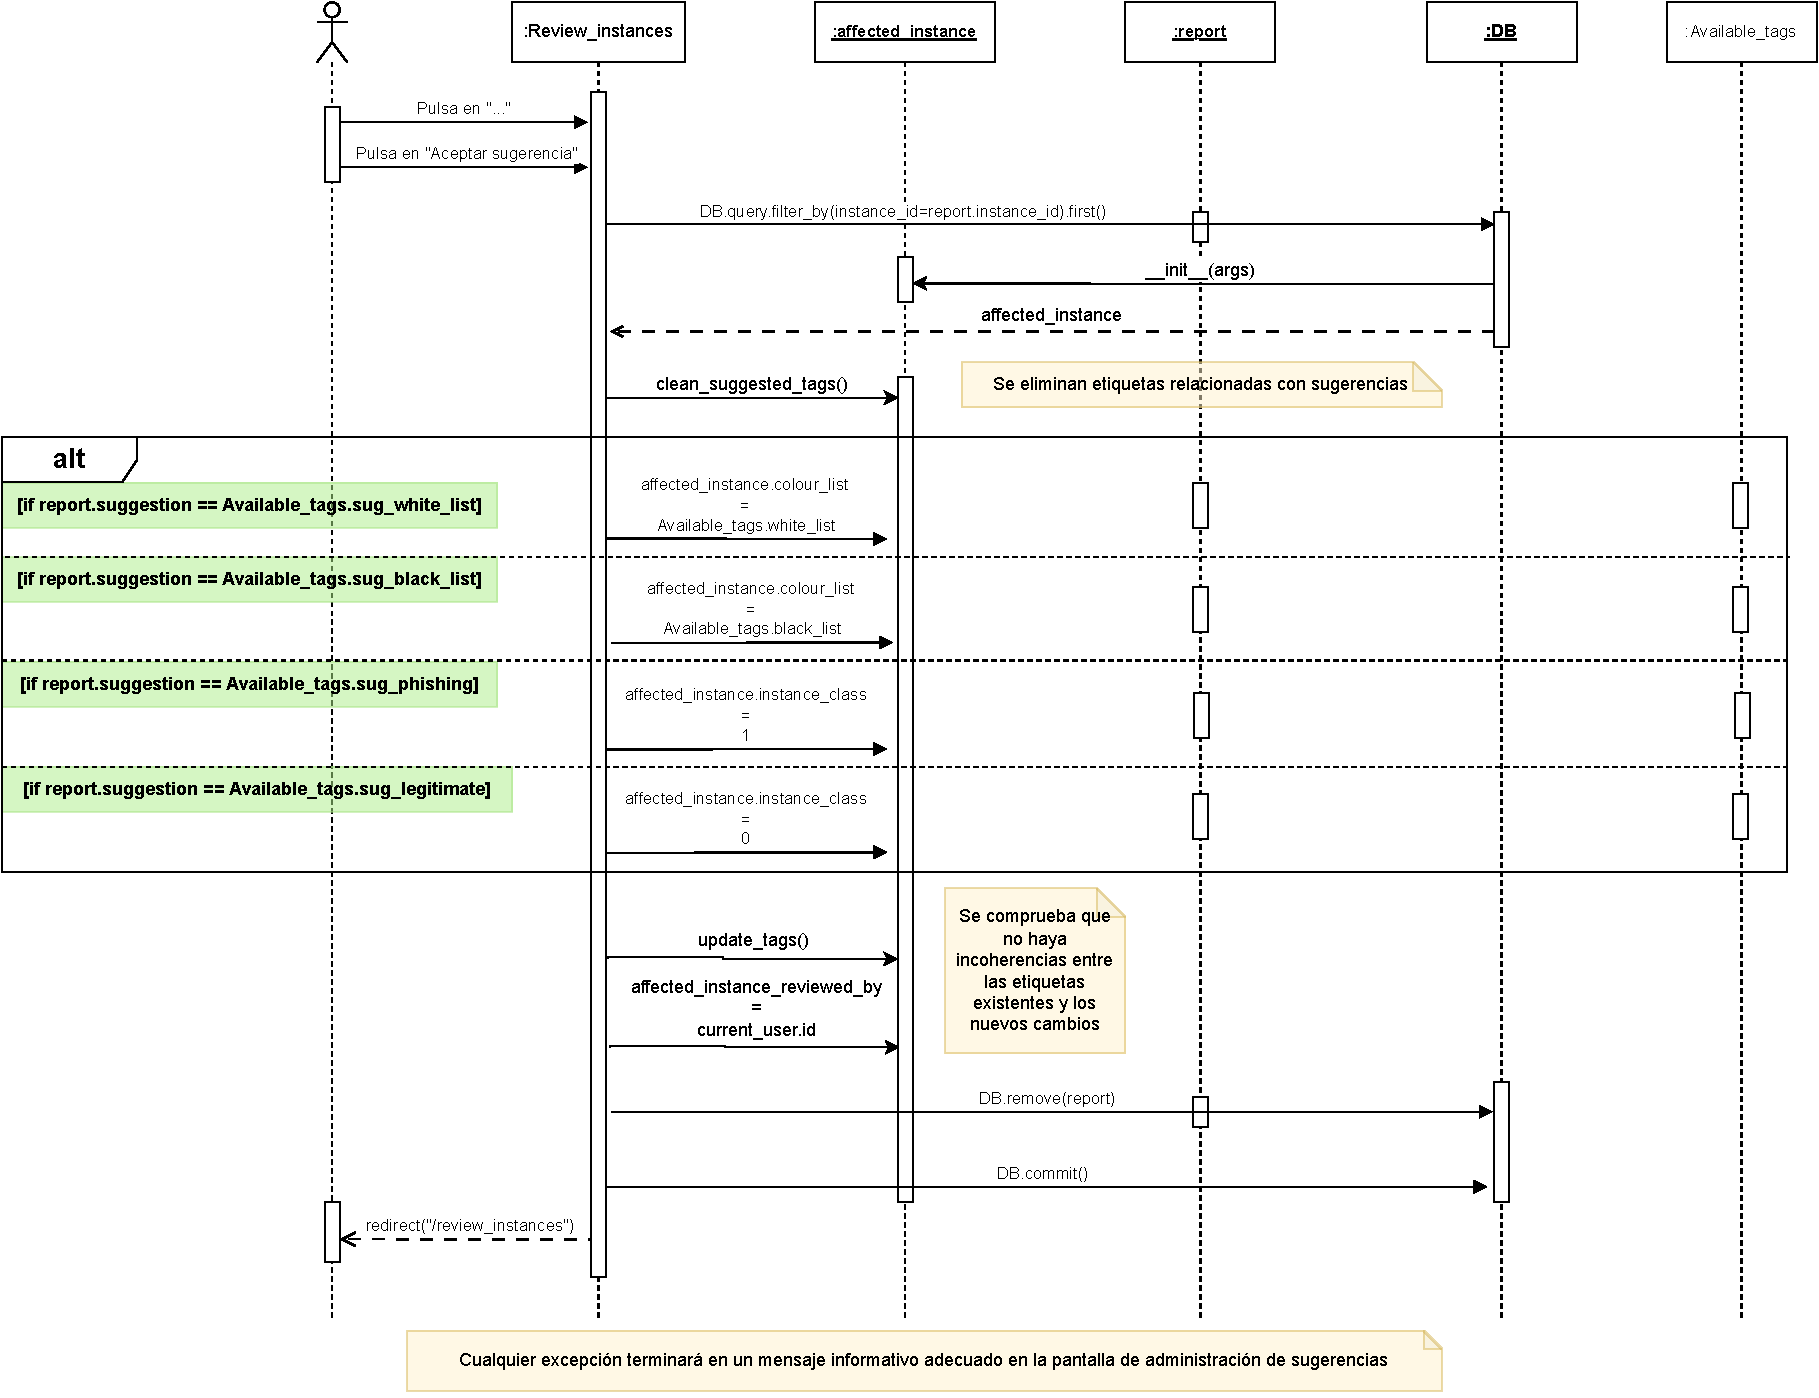
\includegraphics[scale=0.55]{../img/anexos/diagrams/sequence-accept_review}
			\label{c:diagrama-seq-accept-review}
		\end{figure}
	\end{landscape}

\section{Diseño arquitectónico}
\label{s:diseño-arquitectonico}

El diseño arquitectónico de \textit{software} es un proceso que implica la creación de una estructura sólida, funcional y coherente del sistema. Se distinguen dos apartados:

\subsection{Clases}

Un diagrama de clases es una herramienta visual utilizada en la programación orientada a objetos para ilustrar la estructura y las relaciones de clases en un sistema.

Debido a que, como se ha comentado anteriormente, Python es un lenguaje más flexible, en un primer lugar se muestra en el diagrama~\ref{c:classes-general} que representa, en alto nivel, como se relacionan algunas de las clases que controlan las funcionalidades principales de la \textit{web}. Es destacable que se ha utilizado una interpretación propia de UML, adoptando ciertas herramientas visuales pero no siendo estrictos en su uso.

\begin{figure}[h]
	\caption[Diagrama: lógica general]{Diagrama general de la lógica de negocio principal en la aplicación.}
	\centering
	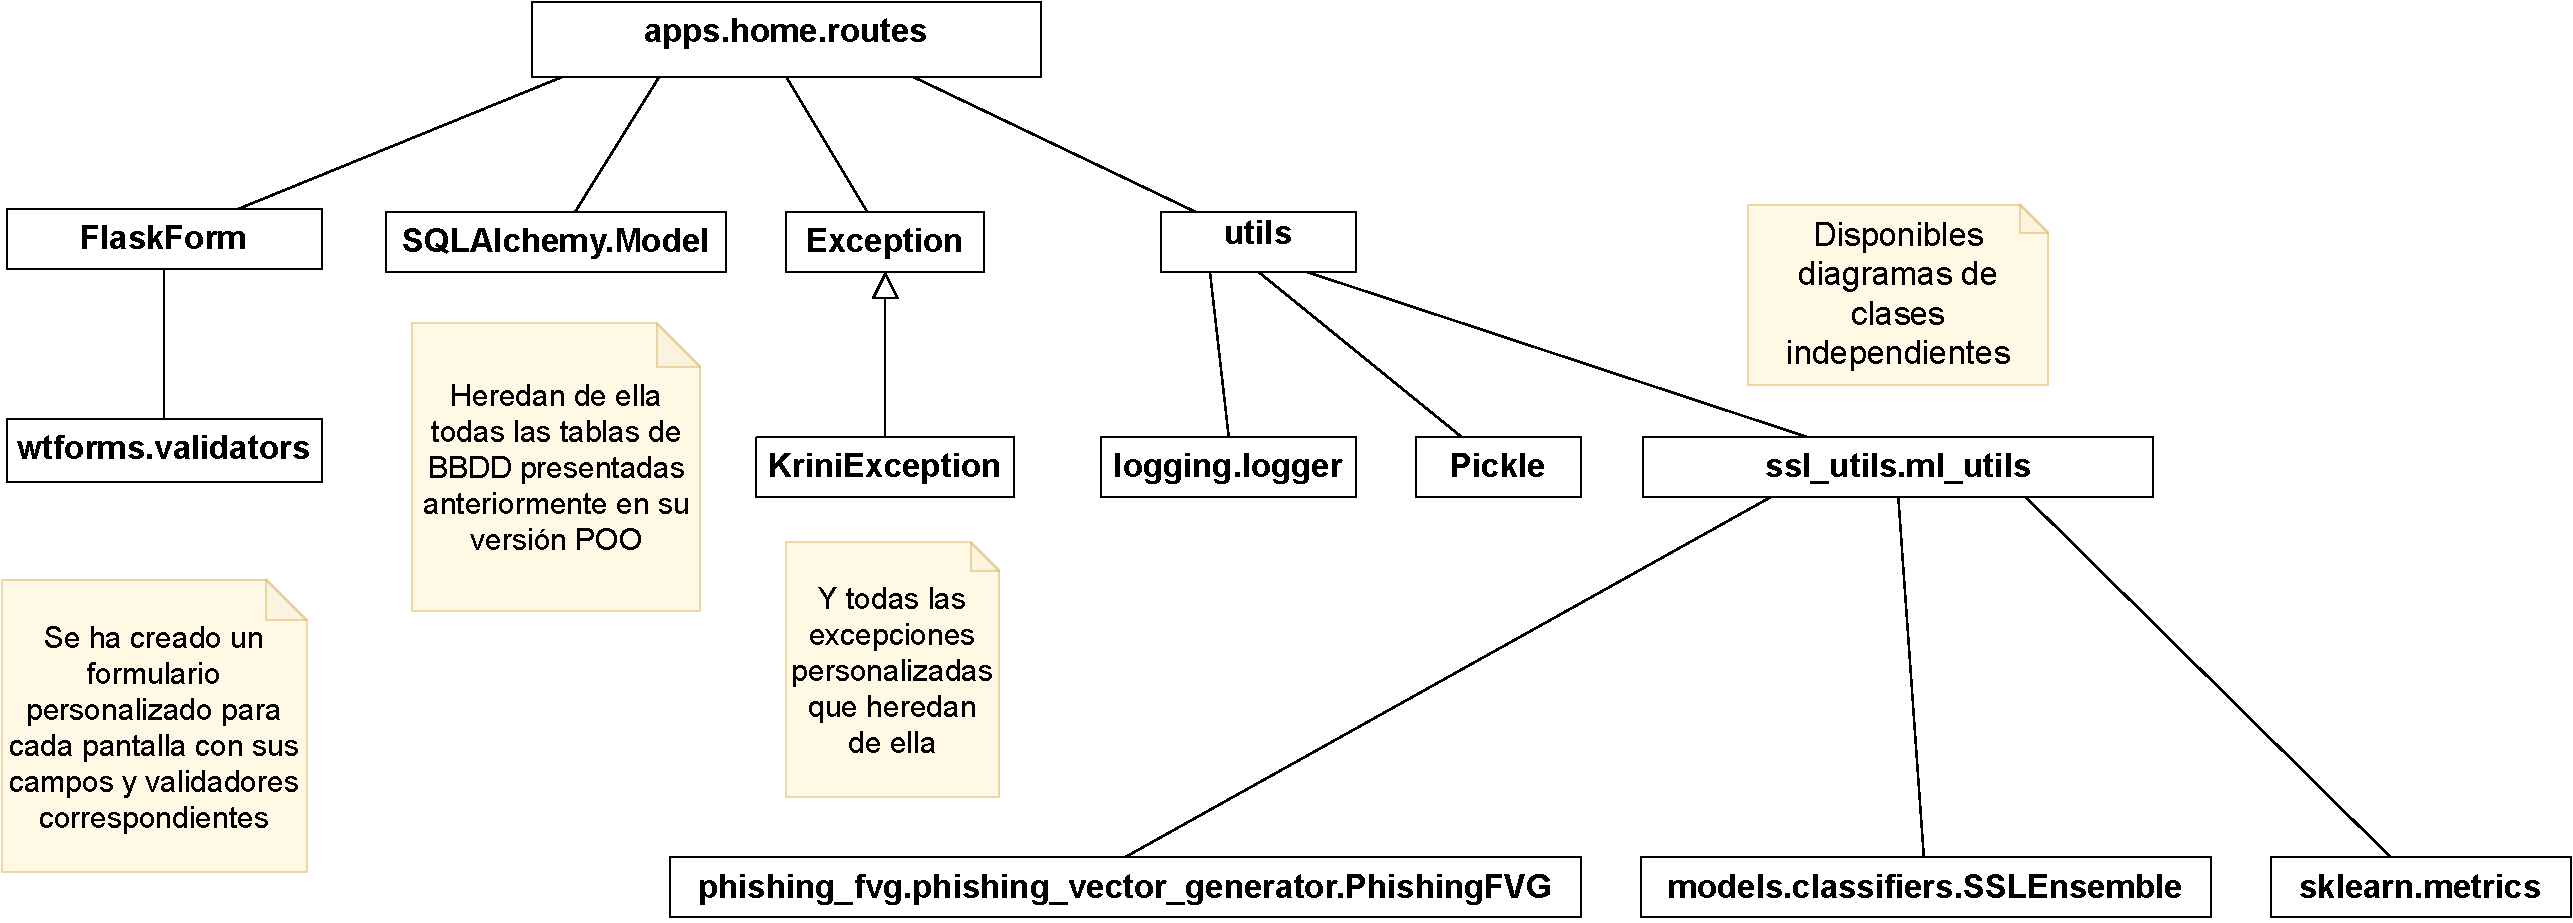
\includegraphics[width=\textwidth]{../img/anexos/diagrams/classes-general}
	\label{c:classes-general}
\end{figure}

Como se puede comprobar, la aplicación utiliza ciertas dependencias, como los formularios de \texttt{Flask}, modelos de datos de \texttt{SQLAlchemy} y excepciones personalizadas, entre otros. Con el fin de fraccionar lo máximo posible el código para facilitar su reutilización, se ha creado un archivo de utilidades que no es una clase (Python permite importar funciones independientes). Este achivo, entre otros, utiliza la clase \texttt{logging}, \texttt{Pickle} y otro archivo de utilidades propio (este en concreto relacionado con ML).

El segundo archivo de utilidades centraliza la lógica relacionada con la obtención de modelos y la gestión de vectores de características. Por eso se relaciona con clases como \texttt{SSLEnsemble} o \texttt{PhishingFVG}. Como estas dos sí son clases <<tradicionales>>, se han generado sus diagramas UML, que se visualizan en las imágenes~\ref{c:classes-ssl} y~\ref{c:classes-fvg} respectivamente.

\begin{figure}[h]
	\caption[Diagrama: clases (\texttt{SSLEnsemble})]{Diagrama de clases correspondiente a \texttt{SSLEnsemble}.}
	\centering
	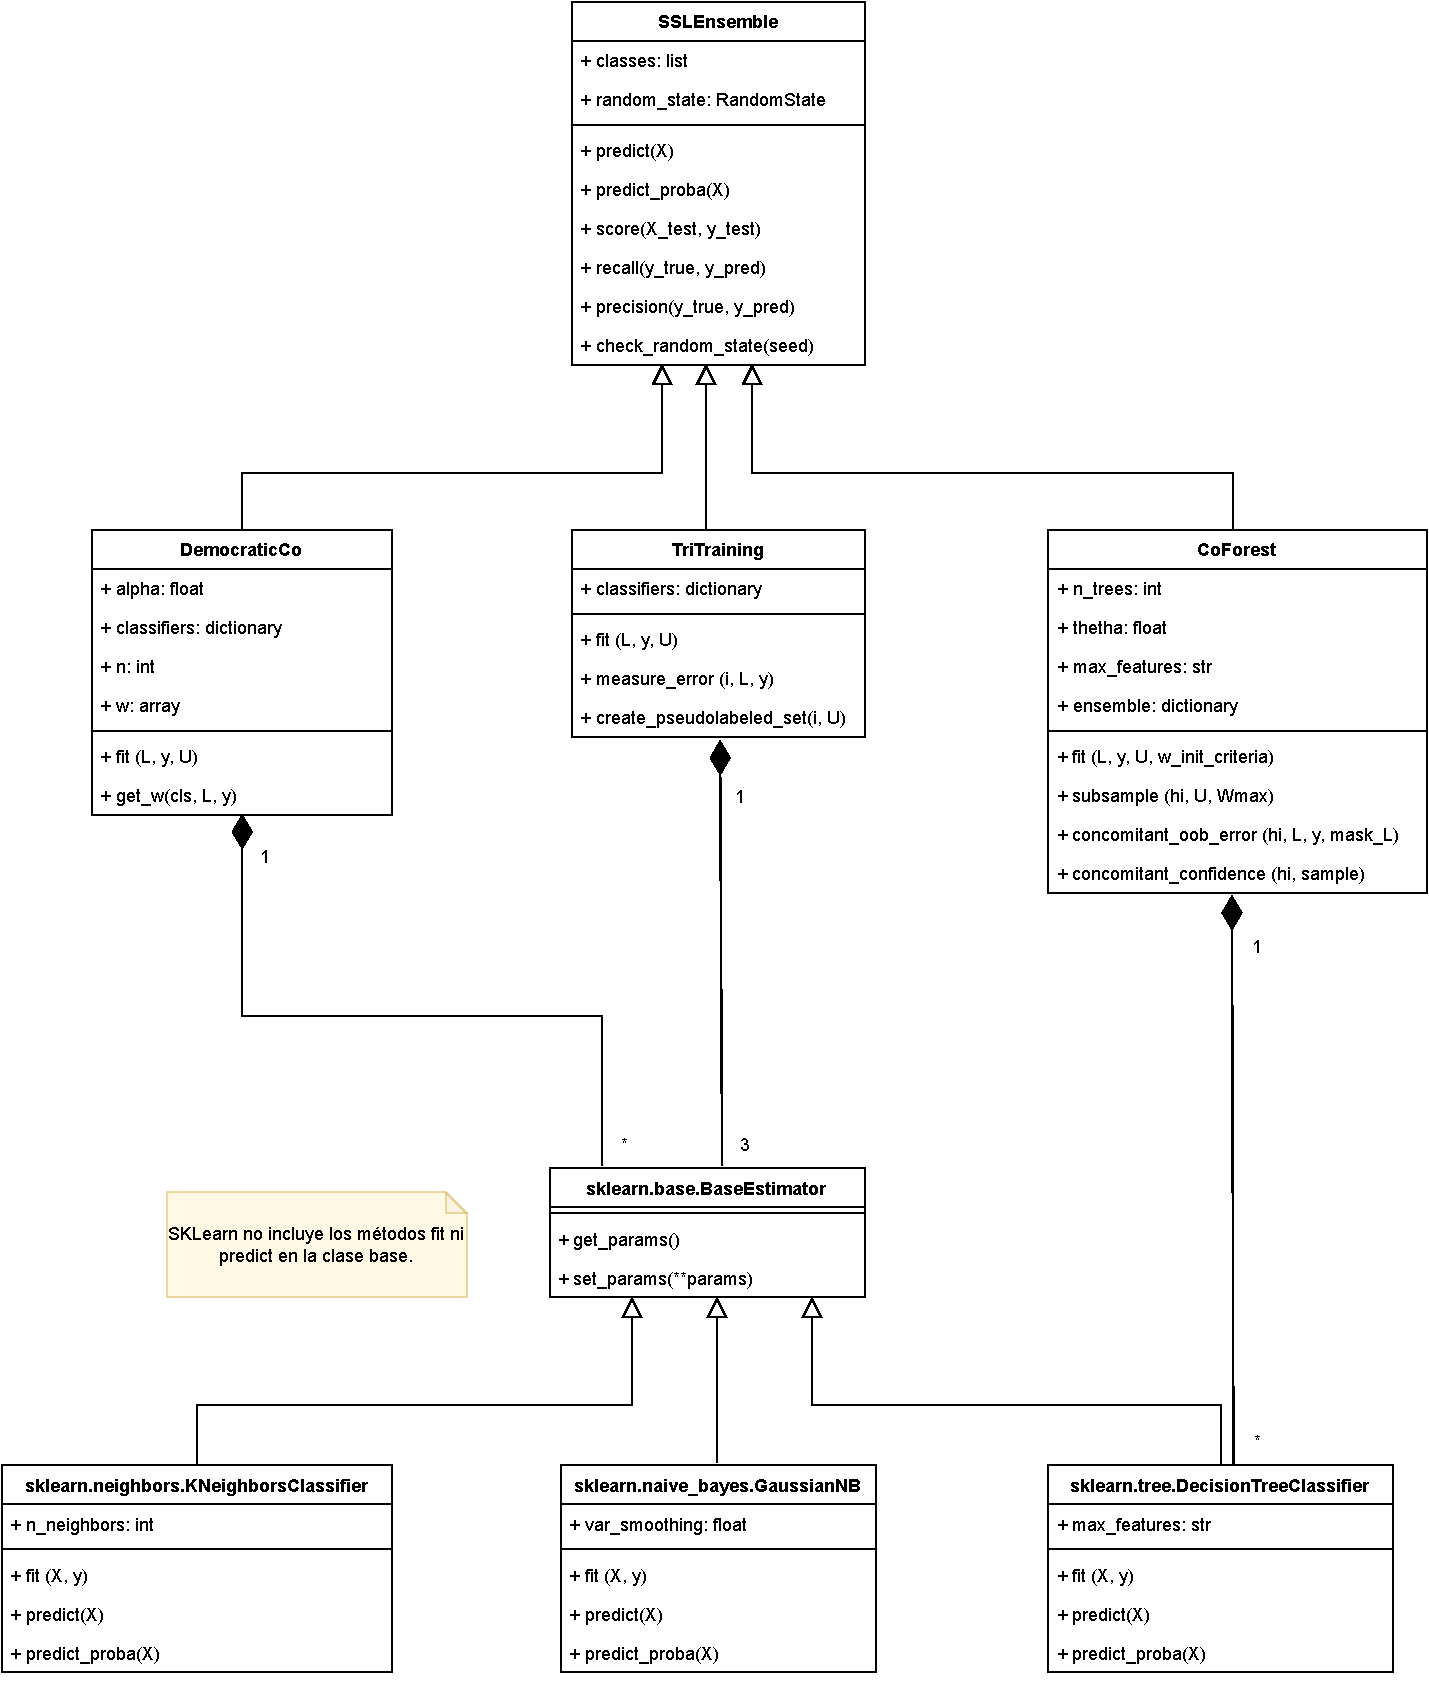
\includegraphics[width=\textwidth]{../img/anexos/diagrams/classes-ssl}
	\label{c:classes-ssl}
\end{figure}

En el diagrama~\ref{c:classes-ssl} se muestra cómo se han implementado los algoritmos de aprendizaje semisupervisado (nótese que no todos los métodos han sido incluidos en el diagrama por cuestiones de visualización). Además, se representa su relación con los clasificadores base de la API de \texttt{SKLearn}.

\begin{figure}[h]
	\caption[Diagrama: clases (\texttt{PhishingFVG})]{Diagrama de clases correspondiente a \texttt{PhishingFVG}.}
	\centering
	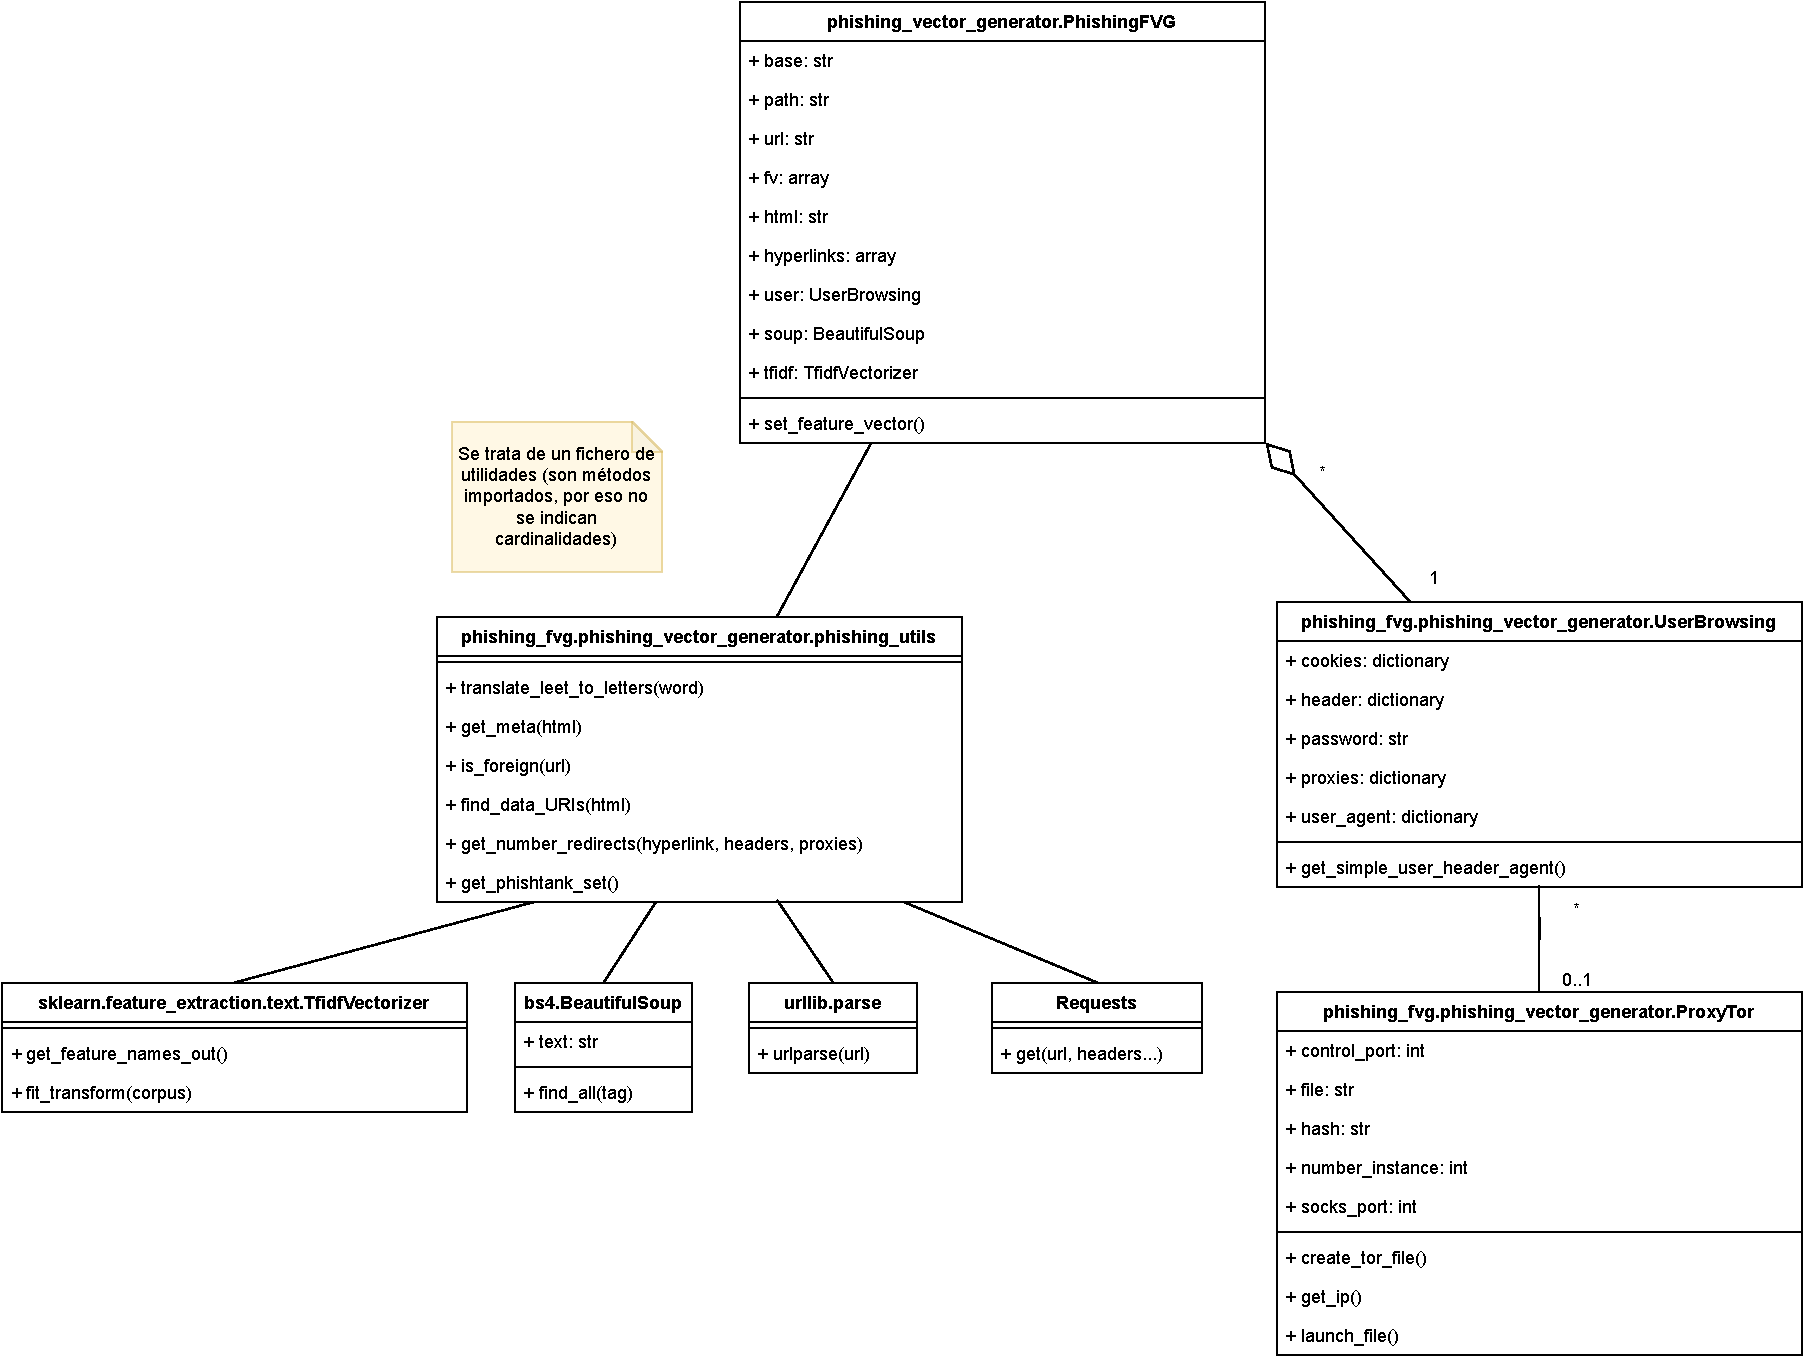
\includegraphics[width=\textwidth]{../img/anexos/diagrams/classes-fvg}
	\label{c:classes-fvg}
\end{figure}

Por último, en el diagrama~\ref{c:classes-fvg} se muestra cómo se ha implementado la extracción de vectores de características. Como se puede observar, hay una clase principal para cada URL analizable que se sirve de un nuevo archivo de utilidades. Este archivo se ha extraído debido a que las funciones que contiene (se muestran algunos ejemplos) son muy generales, por lo que se podrían reutilizar en otros contextos. Nuevamente, no se trata de una clase.

Por otro lado, se ha creado una clase que simula un usuario que navega en \textit{Internet} y almacena campos que pueden ser utilizados junto con la librería \texttt{request} para <<engañar>> las \textit{webs} que se están analizando. Por ejemplo, muchas de ellas son escépticas si les llega una petición sin un \texttt{user-agent} en el encabezado. Para facilitar la limpieza del código, se accede a este tipo de campos a través de la clase \texttt{UserBrowsing}.

Esta, además, está relacionada con la clase \texttt{ProxyTor}, ya que puede ser utilizado (o no) en las peticiones (generalmente se incluye como un parámetro (diccionario) en la petición y se levanta con el \textit{script} auxiliar \texttt{proxies\_launcher.py}). Por cuestiones de seguridad, esta opción es especialmente interesante cuando se genera un \textit{dataset} de \textit{phishing}.

\subsection{Despliegue}

En la figura~\ref{c:diagrama-deploy} se muestra el diagrama de despliegue de la aplicación. Como se puede comprobar, se ha optado por una arquitectura cliente-servidor. Además, se ha establecido un patrón de tres niveles, donde el cliente actúa como controlador de la vista de usuario, el servidor implementa la lógica de aplicación y, por último, el servidor de base de datos gestiona la capa de persistencia.

\begin{figure}[h]
	\caption[Diagrama: despliegue]{Diagrama de despliegue de la aplicación.}
	\centering
	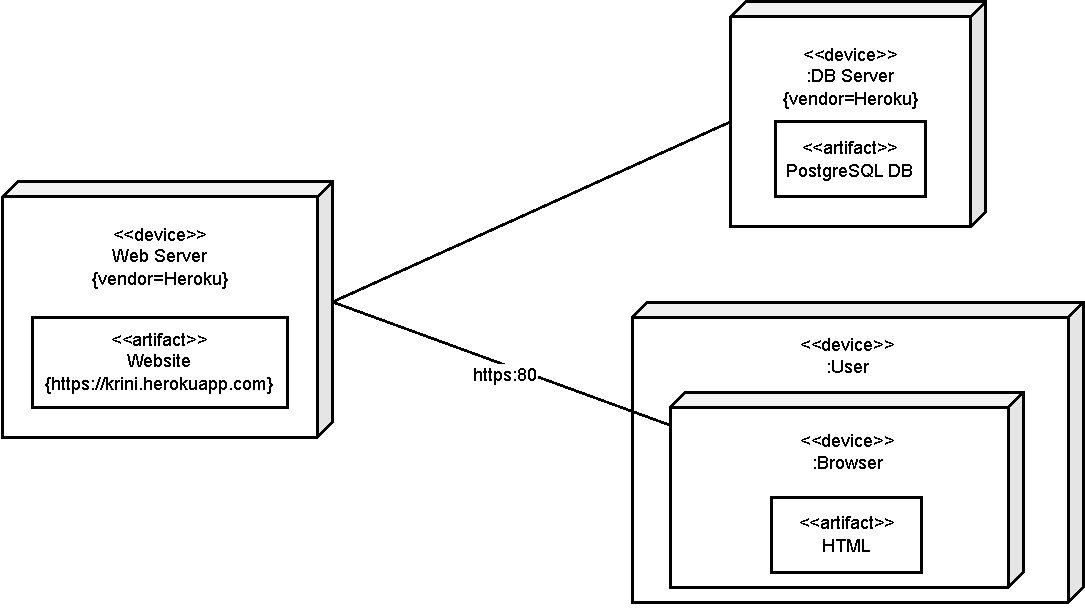
\includegraphics[width=\textwidth]{../img/anexos/diagrams/deploy}
	\label{c:diagrama-deploy}
\end{figure}
\apendice{Documentación técnica de programación}

\section{Introducción}

\section{Estructura de directorios}

\section{Manual del programador}

\section{Compilación, instalación y ejecución del proyecto}

\section{Pruebas del sistema}

\apendice{Documentación de usuario}

\section{Introducción}

En este anexo se pretende describir de forma concisa las características y funcionalidades de la \textit{web} desarrollada, además de los requisitos necesarios para su correcta renderización.

Es importante destacar que la \textit{web} ha sido desplegada en Heroku. Sin embargo, esta PaaS, tiene importantes restricciones en las versiones para estudiantes. En concreto, Krini se ve gravemente perjudicada ya que Heroku cancela toda petición que dure más de 30 segundos (lo que impide, en la mayoría de los enlaces, realizar un análisis completo).

Por este motivo, también se va a documentar cómo desplegar la aplicación en local (servidor de producción y base de datos) mediante contenedores de Docker.

\section{Requisitos de usuarios}

En este apartado se pretenden enumerar los requisitos necesarios para acceder correctamente a la \textit{web} desarrollada.

\subsection{Requisitos Heroku}
\label{s-e:requisitos-heroku}

Los requisitos en este caso vienen limitados por el uso de las bibliotecas \texttt{Chart.js} (v2.9.3) y \texttt{Bootstrap} (v4.4.1). En este caso, se necesita que la \textit{web} se renderice en navegadores con las siguientes versiones:

\begin{itemize}
	\item \textbf{Google Chrome:} todas las versiones modernas.
	\item \textbf{Mozilla Firefox:} todas las versiones modernas.
	\item \textbf{Safari:} todas las versiones modernas.
	\item \textbf{Microsoft Edge:} todas las versiones modernas.
	\item \textbf{Internet Explorer:} versión 10 o superior.
\end{itemize}

\subsection{Requisitos Docker}
\label{s-e:requisitos-docker}

Además de los requisitos expuestos en la sección~\ref{s-e:requisitos-heroku}, si se quiere ejecutar el contenedor de Docker en local, se ha de cumplir con las siguientes características en función del sistema operativo. Es relevante que, como se puede comprobar en el diagrama de despliegue de Docker (disponible en la ilustración~\ref{c:diagrama-deploy-docker}), los contenedores de la base de datos y de la \textit{web} son independientes. Por ello, se ha de contar con el \textit{plugin} \texttt{docker-compose}.

\begin{enumerate}
	\item \textbf{Windows}: se recomienda utilizar Docker Desktop por su simplicidad. Los requisitos completos se pueden consultar en su documentación oficial\footnote{Disponible en \url{https://docs.docker.com/desktop/install/windows-install/}}. Sin embargo, se resumen a continuación:
	
	\begin{itemize}
		\item \texttt{WLS}
		\item Procesador de 64 bits
		\item 4GB de memoria RAM
		\item 3GB de memoria para las imágenes
		\item El \textit{plugin} \texttt{docker-compose} viene por defecto con la versión de escritorio.
	\end{itemize}

	\item \textbf{Linux}: nuevamente, los requisitos completos se facilitan en la documentación\footnote{Disponible en \url{https://docs.docker.com/desktop/install/linux-install/}}. En resumen, se recomienda:
	\begin{itemize}
		\item Disponer de soporte para virtualización
		\item Procesador de 64 bits
		\item 4GB de memoria RAM
		\item 3GB de memoria para las imágenes
		\item Instalar el \textit{plugin} \texttt{docker-compose} mediante \texttt{\$ sudo apt-get install docker-compose-plugin} (en Ubuntu y Debian) o \texttt{\$ sudo yum install docker-compose-plugin} (en distribuciones basadas en RPM).
	\end{itemize}
\end{enumerate}



\section{Instalación}

La instalación de un producto \textit{software} es el proceso mediante el cual se configura y prepara un programa o aplicación para que pueda ser utilizado en un dispositivo objetivo.

Debido a que la aplicación desarrollada es una \textit{web}, no hace falta pasar por este proceso. Sin embargo y debido a las restricciones de Heroku anteriormente mencionadas, se va a explicar cómo desplegar la aplicación en local mediante Docker (con servidores de producción) para comprobar la funcionalidad al completo. Se recuerda que las instrucciones para levantar el servidor de desarrollo se encuentran en la sección~\ref{s-d:flask-deploy}.

\subsection{Acceso mediante Heroku}

Simplemente se ha de acceder mediante el navegador introduciendo la dirección \url{https://krini.herokuapp.com/}

\subsection{Despliegue en Docker}
\label{s-e:docker-deploy-users}

Para facilitar que cualquier usuario pueda desplegar un contenedor de Docker (en realidad, dos) y levantar su propio servidor de gunicorn en local sin tener conocimientos técnicos, se han preparado unos \textit{scripts} multiplataforma disponibles en \url{https://github.com/phf1001/semisupervised-learning-in-cibersecurity/tree/main/docker-deploy-kit}

De esta forma, tan solo se debe seleccionar el sistema operativo anfitrión, descargar los archivos (se facilita un comprimido con todos incluidos) y garantizar que se cumple con los requisitos de la sección~\ref{s-e:requisitos-docker}.

Para levantar el servidor en local y garantizar que la base de datos se rellena completamente, se han de seguir los siguientes pasos teniendo en cuenta que los \textit{scripts} en Linux se ejecutan mediante el comando \texttt{\$ sh nombre-script.sh} y en Windows mediante \texttt{\$ nombre-script.bat}.

\begin{enumerate}
	\item Ubicarse en la carpeta donde se encuentren los \textit{scripts}.
	\item Si es la primera vez que se ejecuta:
	\begin{enumerate}
	\item Lanzar el script \texttt{docker-first-time-1} y seguir las instrucciones (esperar 30 segundos y abrir el navegador cuando lo indique).
	\item Ejecutar el \textit{script} \texttt{docker-first-time-2} y respetar los pasos indicados (esperar 30 segundos antes de abrir el navegador).
	\end{enumerate}
	\item Si se quieren parar los contenedores para reutilizarlos luego, ejecutar el \textit{script} \texttt{docker-stop} y \texttt{docker-start} para volver a iniciarlos.
	\item Si se quieren borrar las imágenes y contenedores del sistema definitivamente, ejecutar el \textit{script} \texttt{docker-clean}
\end{enumerate}

\textbf{Importante}: iniciar el demonio de Docker antes de lanzar los \textit{scripts}. En Windows basta con ejecutar la aplicación de escritorio.

\section{Manual del usuario}

En este punto del manual se supone que todos los usuarios tienen acceso a la aplicación, ya sea mediante un contenedor de Docker o Heroku.

A continuación, se procede a ilustrar las funcionalidades básicas de la \textit{web}. Es destacable que no todos los usuarios cuentan con acceso a todas las funcionalidades (consultar diagrama de casos de uso~\ref{b:diagrama-cu}). Por ello, se recomienda probar el producto con una cuenta con permisos de administración.


\subsection{Analizador}
\label{s-e:analizador}

\begin{figure}[h]
	\caption[Manual de usuario: página principal]{Página principal de la aplicación.}
	\centering
	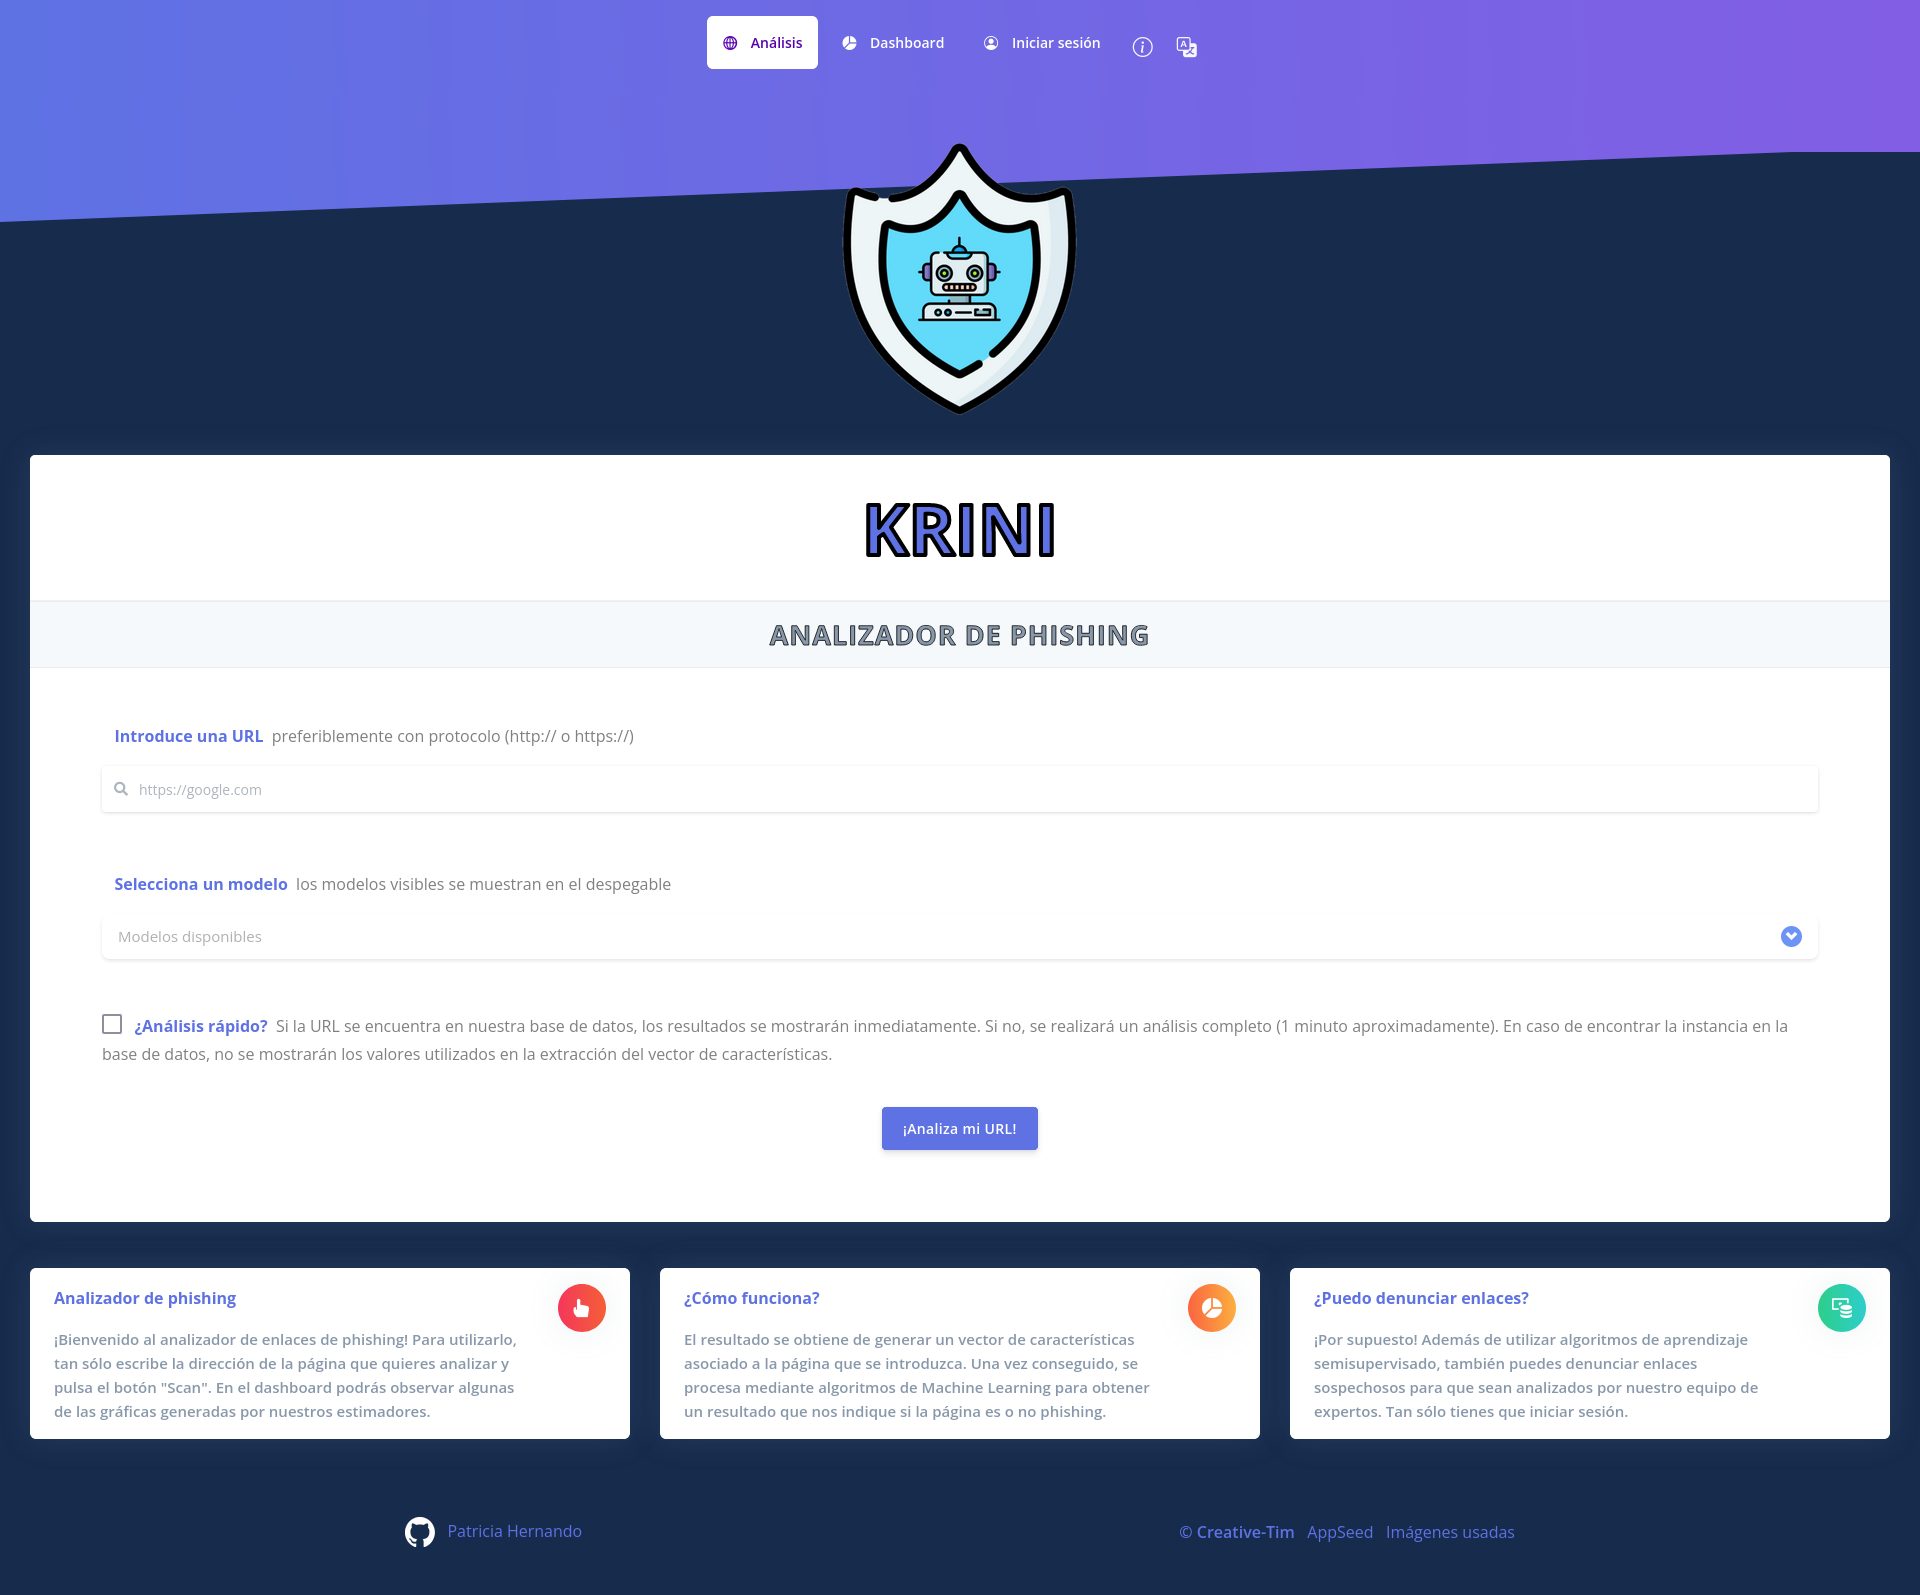
\includegraphics[width=\textwidth]{../img/anexos/user_guide/1_index}
	\label{e-1:index}
\end{figure}

En la ilustración~\ref{e-1:index} se muestra la página principal del analizador disponible para cualquier usuario. Para escanear una URL, basta con introducirla en el campo correspondiente. Es preferible introducir la dirección tal y como aparece en el navegador, pero si no es posible, la aplicación tratará de autocompletarla.

A continuación se pueden seleccionar los clasificadores que se deseen en el desplegable. Si no se selecciona ninguno, se analizará con el modelo por defecto, y en caso de que no exista, con uno aleatorio.

Opcionalmente se puede marcar la casilla <<análisis rápido>>. En este caso, no se extraerá el vector de características si ya existe en la base de datos\footnote{Para garantizar que la base de datos se autocompleta, cualquier vector de características nuevo que se extraiga por un usuario registrado se guardará en la sección de <<instancias>> (consultar sección~\ref{s-e:instances} del manual) con etiquetas adecuadas (\texttt{new-instance}, \texttt{auto-classified} y \texttt{recommendation-review}) (consultar imagen~\ref{e-6:more-labels}) y se incluirá una sugerencia para su revisión (\texttt{suggestion-review-new-scanned}).}.
 
Tras pulsar el botón de analizar, se mostrará una pantalla de carga mientras se extrae el vector de características correspondiente a la URL introducida (imagen~\ref{e-1:analysis}). En caso de error, se volverá a la página principal con un mensaje informativo.

\begin{figure}[h]
	\caption[Manual de usuario: página de carga]{Página de análisis de URL.}
	\centering
	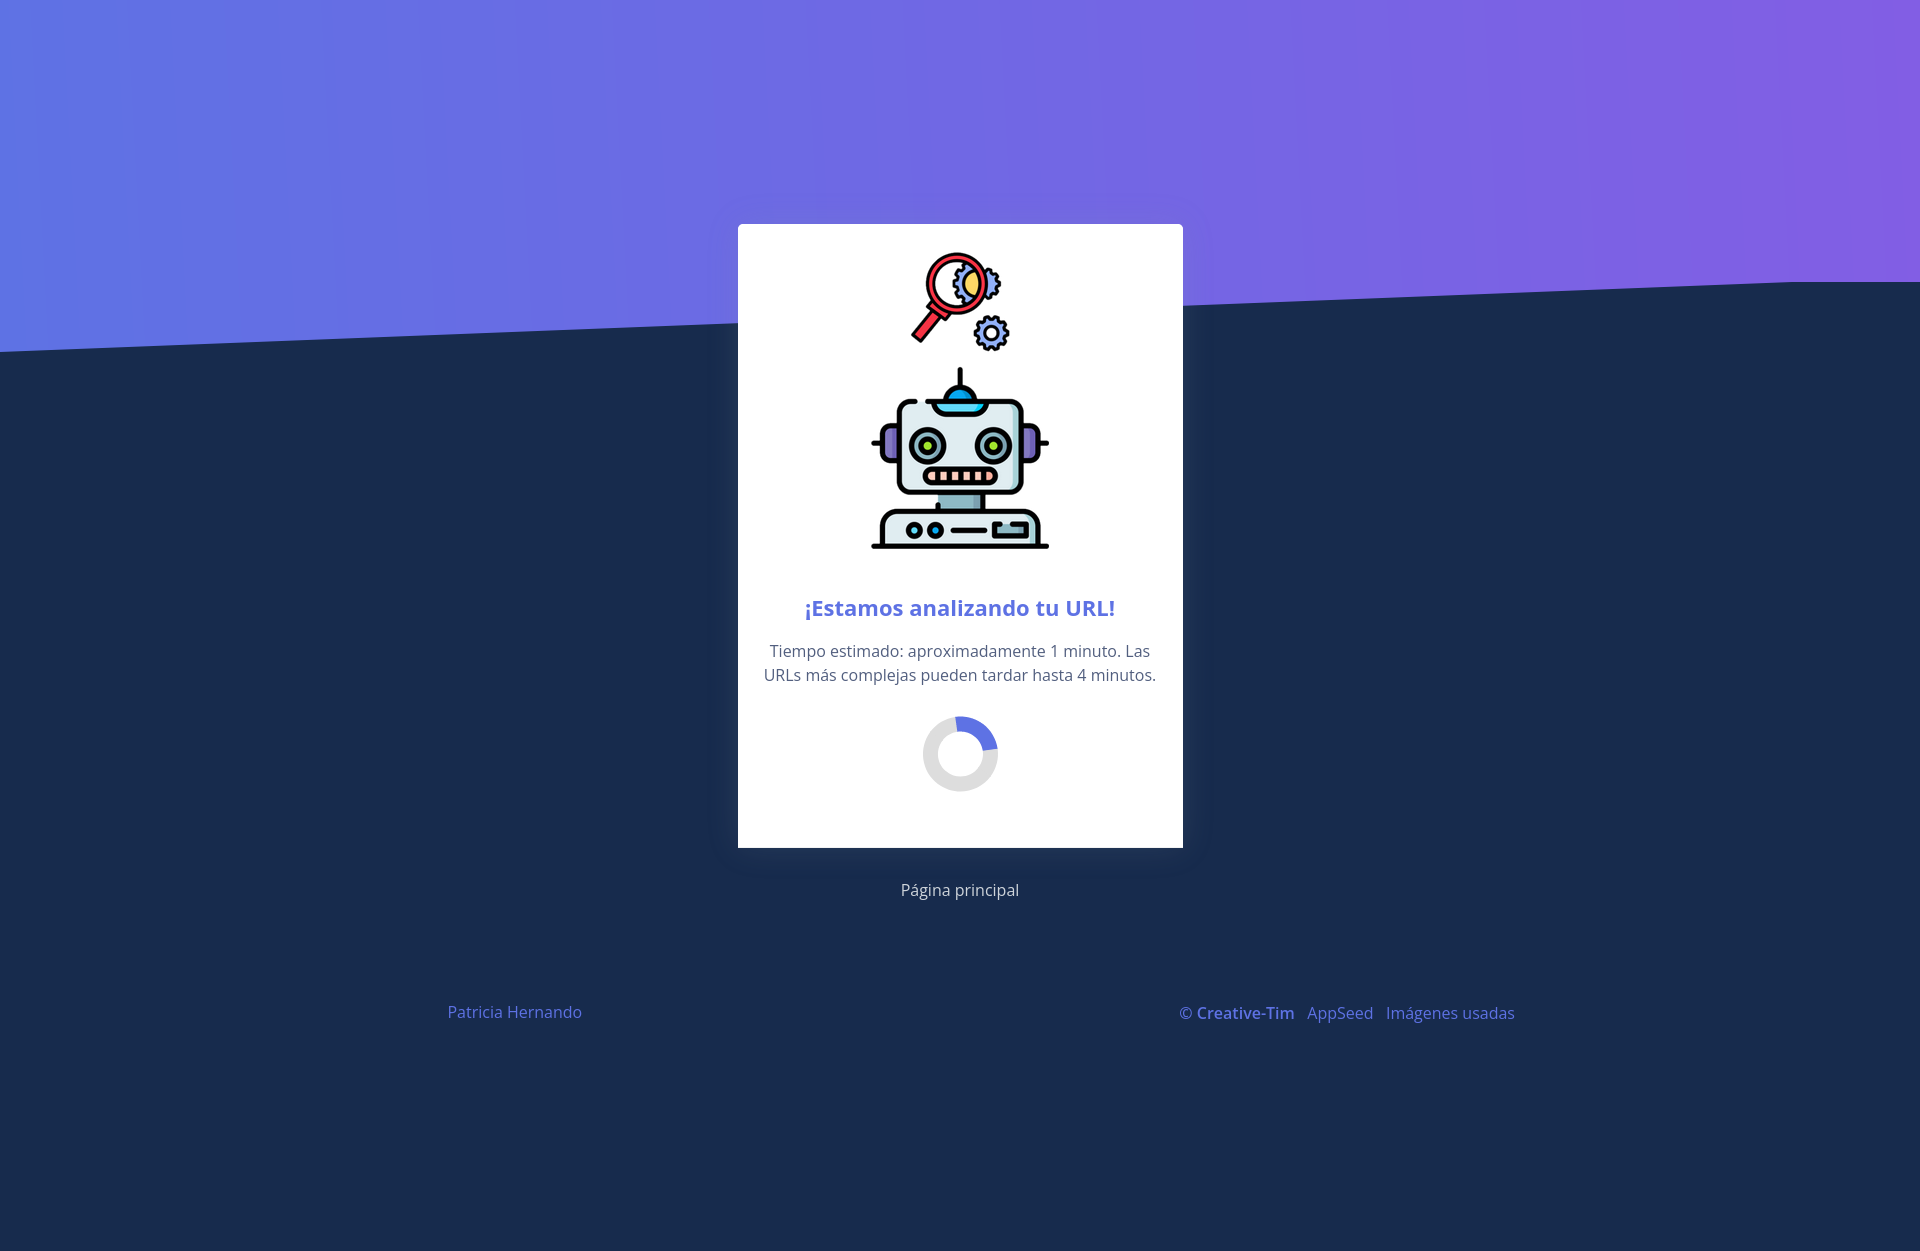
\includegraphics[width=\textwidth]{../img/anexos/user_guide/2_analysis}
	\label{e-1:analysis}
\end{figure}

\subsection{\textit{Dashboard}}
\label{s-e:dashboard}

En el \textit{dashboard} se pueden observar los resultados de analizar la URL introducida mediante los clasificadores seleccionados.

Las gráficas interactivas (imagen~\ref{e-3:dashboard-1}) se muestran tanto si se ha realizado un análisis rápido como si no. En un primer lugar se realiza una comparativa entre clasificadores. A continuación, se representa en un gráfico de tipo \textit{doughnut} las predicciones de todos los estimadores y en una tabla la seguridad de cada clasificador en la predicción. Por último, se pueden contemplar individualmente las estadísticas de cada clasificador en la gráfica giratoria (pulsar el botón <<siguiente>> para cambiar entre gráficas).

\begin{figure}[h]
	\caption[Manual de usuario: gráficas del \textit{dashboard}]{\textit{Dashboard} mostrado tras un análisis.}
	\centering
	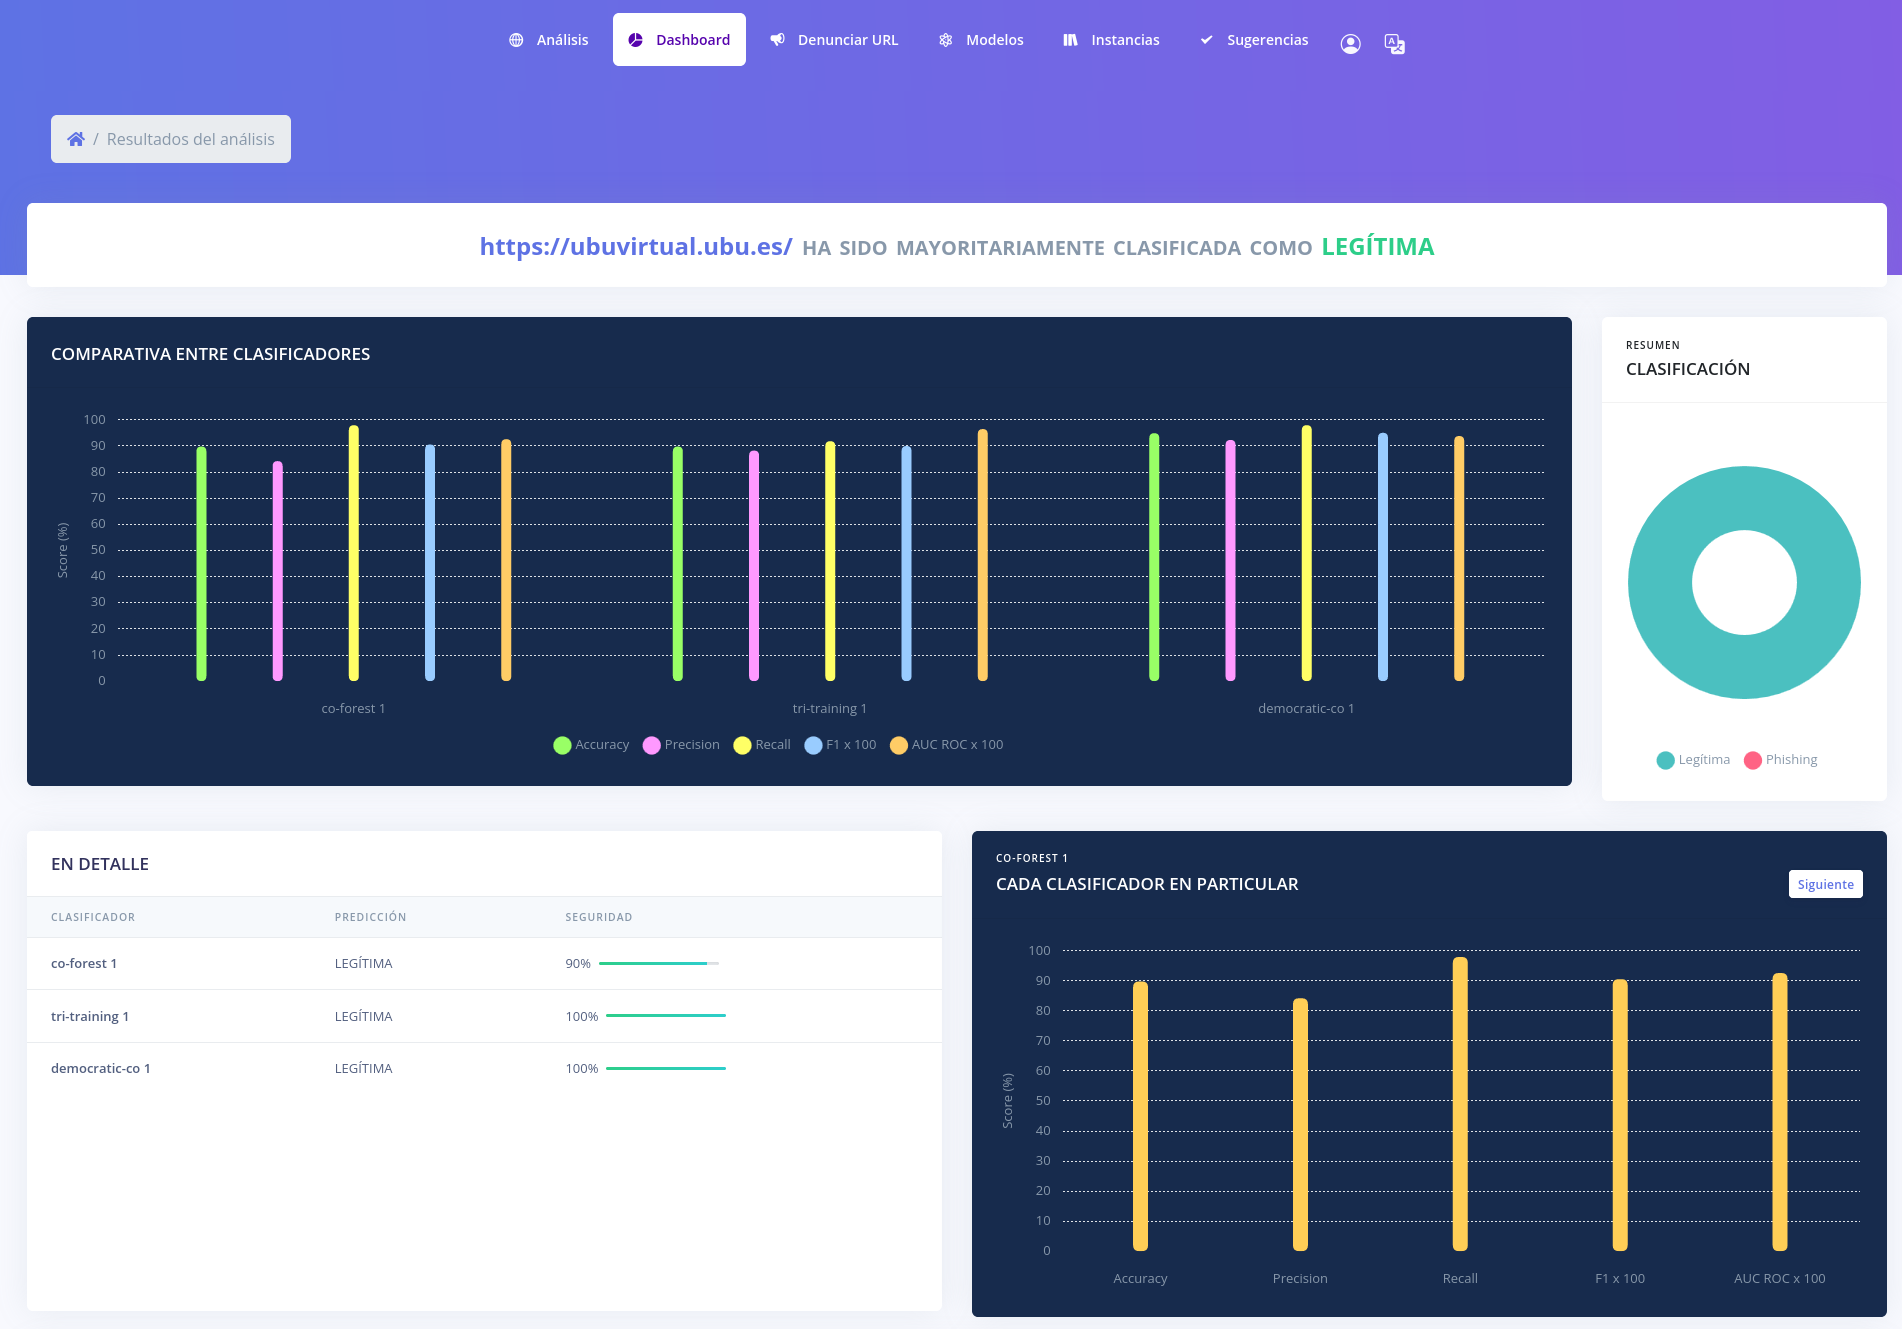
\includegraphics[width=\textwidth]{../img/anexos/user_guide/3_dashboard_1}
	\label{e-3:dashboard-1}
\end{figure}

Si no se ha realizado un análisis rápido, también se mostrará cómo se ha obtenido el vector de características de la URL. Un ejemplo se puede visualizar en la captura~\ref{e-3:dashboard-2}. Pulsando en el icono de la bombilla, se activará un desplegable que muestra información sobre cada característica.

\begin{figure}[h]
	\caption[Manual de usuario: vector de características en el \textit{dashboard}]{Análisis del vector de características mostrado en el dashboard.}
	\centering
	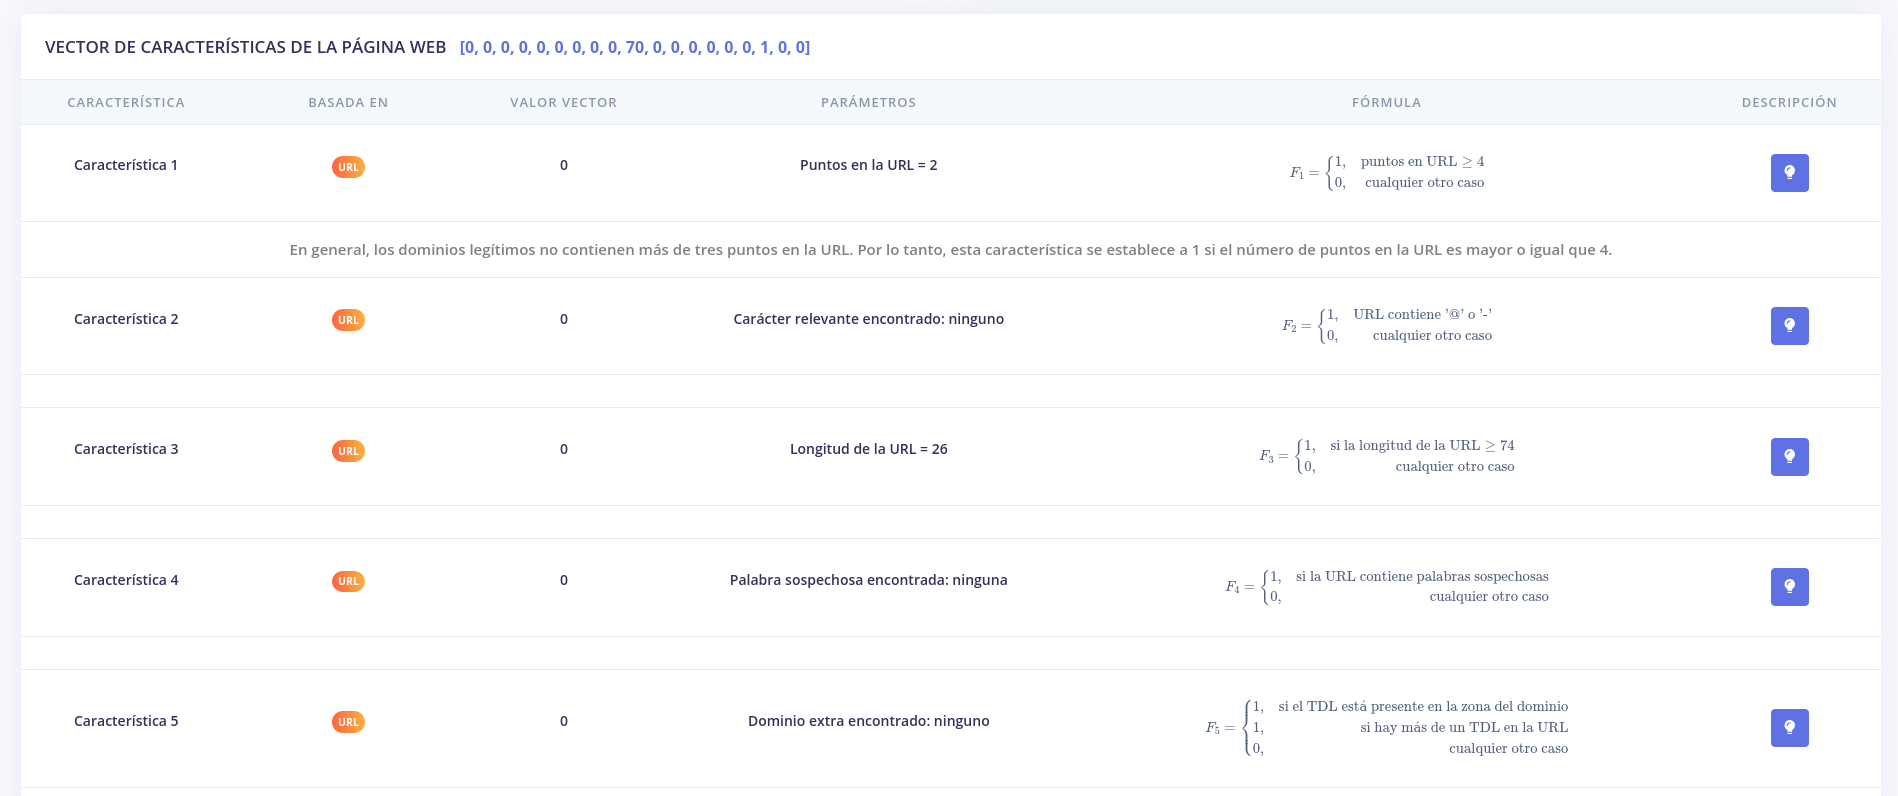
\includegraphics[width=\textwidth]{../img/anexos/user_guide/3_dashboard_2}
	\label{e-3:dashboard-2}
\end{figure}

\begin{figure}[h]
	\caption[Manual de usuario: reportar análisis erróneo]{Reportar análisis realizados erróneamente.}
	\centering
	
\includegraphics[width=\textwidth]{../img/anexos/user_guide/3_report_false_analysis}
	\label{e-3:report-false-analysis}
\end{figure}

\label{s-e:report-false-analy}
La última funcionalidad del \textit{dashboard} consiste en reportar análisis erróneos. Si se opina que una URL ha sido clasificada incorrectamente, se puede notificar a los administradores pulsando en el botón correspondiente (imagen~\ref{e-3:report-false-analysis}). Posteriormente, ellos podrán utilizar esta información para crear nuevos modelos o tomar las medidas que consideren oportunas. La notificación estará disponible en el apartado de <<sugerencias>> (consultar la sección~\ref{s-e:sugerencias} del manual).

\subsection{Denunciar URL}
\label{s-e:report-url}

Si se está seguro de que una URL pertenece a una lista blanca o negra (es decir, se trata de una página legítima o \textit{phishing} confirmada), se puede reportar para que sea revisada por los administradores (consultar la sección~\ref{s-e:sugerencias} del manual) en el formulario <<denunciar URL>>. Para ello, únicamente habrá que introducir la URL y el tipo de lista a la que pertenece como se muestra en la imagen~\ref{e-3:report-url}.

\begin{figure}[h]
	\caption[Manual de usuario: reportar pertenencia a lista]{Página para reportar pertenencia a lista blanca o lista negra.}
	\centering
	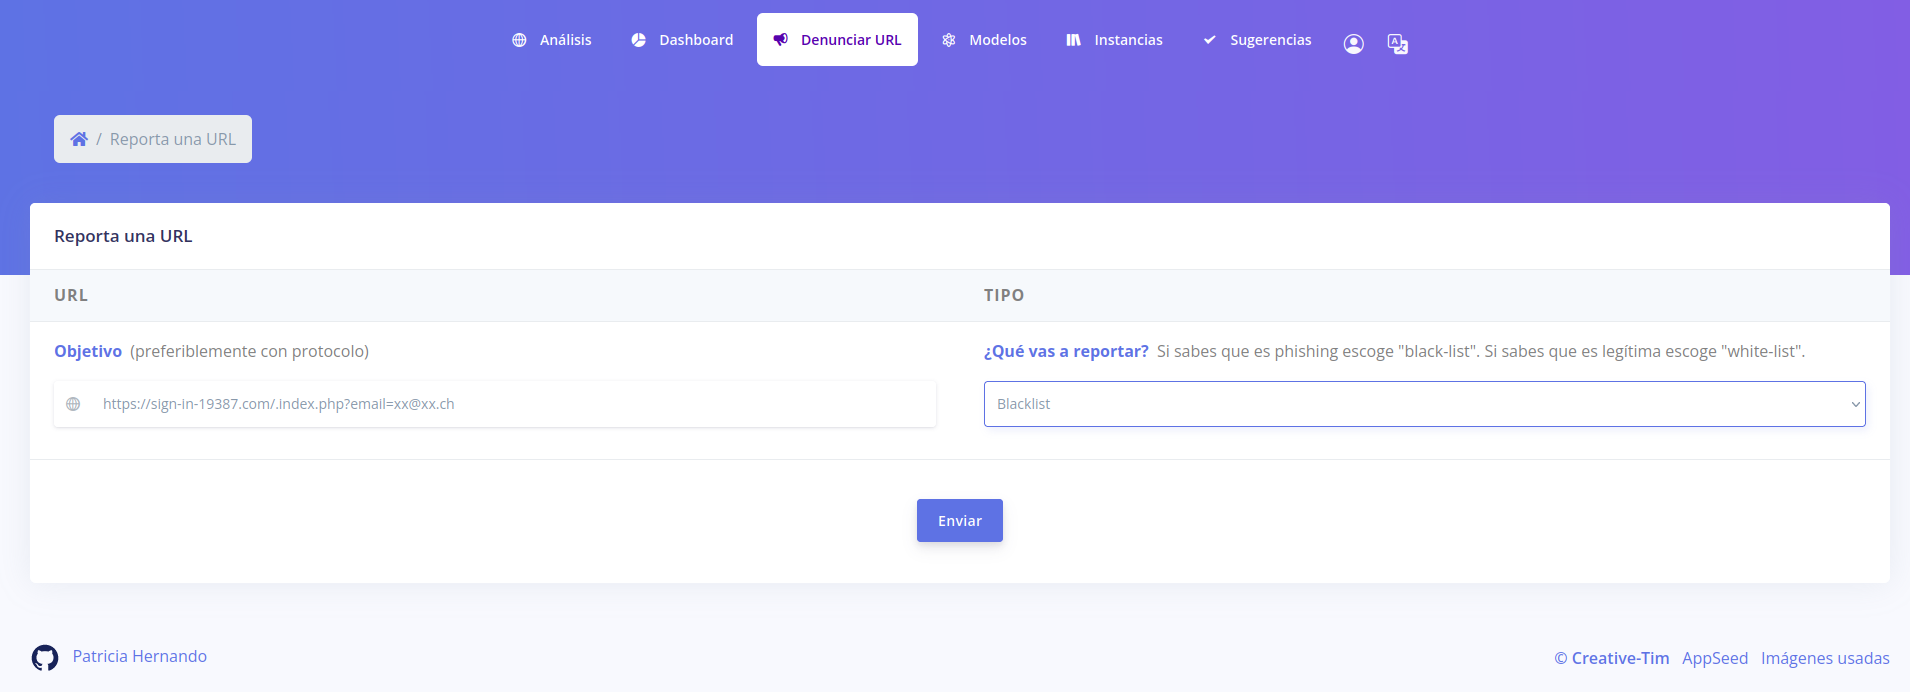
\includegraphics[width=\textwidth]{../img/anexos/user_guide/4_report_url}
	\label{e-3:report-url}
\end{figure}

En caso de que la URL no exista previamente, será incluida en la sección de <<instancias>> (consultar sección~\ref{s-e:instances} del manual), aunque no se generará su vector de características para evitar que el usuario tenga que esperar (como se muestra en la imagen~\ref{e-6:more-labels}) ni se asignará una etiqueta. Posteriormente los administradores podrán ejecutar esta tarea (y el campo \texttt{revisor} pasará a tener el nombre del administrador en lugar de <<?>>). Es destacable que las URL sin vector de características no podrán ser utilizadas para realizar análisis rápidos ni entrenar o evaluar modelos.

\begin{figure}[h]
	\caption[Manual de usuario: ejemplos de etiquetas]{Instancias con variedad de etiquetas. En esta imagen, \texttt{https://ubuvirtual.ubu.es/} ha sido analizada por un usuario registrado y guardada automáticamente por no existir previamente en la base de datos, mientras que \texttt{https://www.naturaselection.com/es/} es el resultado de una URL denunciada que no existía previamente (el reporte se encuentra en las <<sugerencias>> y por este motivo no dispone de vector ni clase). Debido a que no han sido comprobadas por ningún administrador, ambas contienen como revisor <<?>>.}
	\centering
	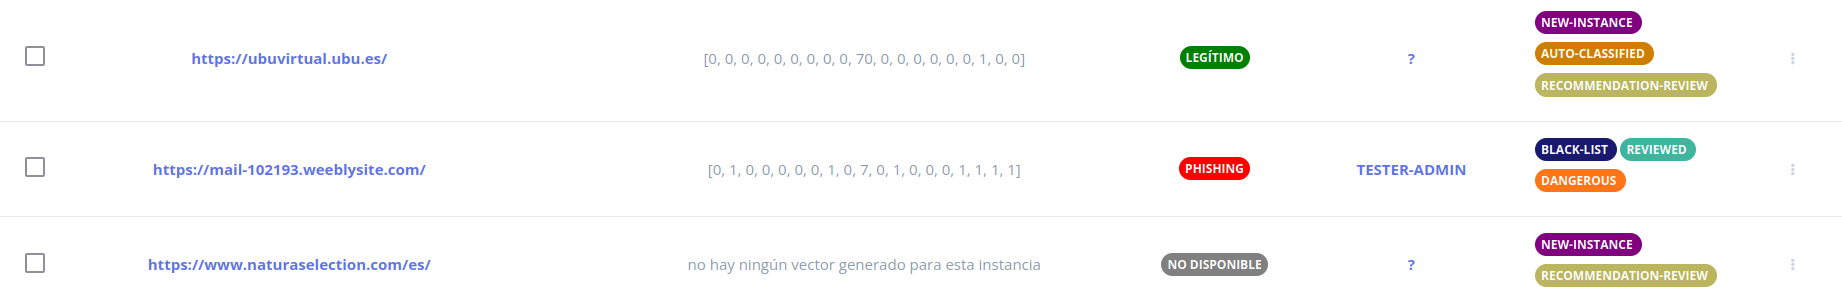
\includegraphics[width=\textwidth]{../img/anexos/user_guide/6_instances_more_labels}
	\label{e-6:more-labels}
\end{figure}


\subsection{Modelos}
\label{s-e:models}

Los administradores podrán gestionar todos los modelos de aprendizaje disponibles en la sección de <<modelos>> (imagen~\ref{e-5:models}).

\begin{figure}[h]
	\caption[Manual de usuario: página de modelos]{Página de administración de modelos.}
	\centering
	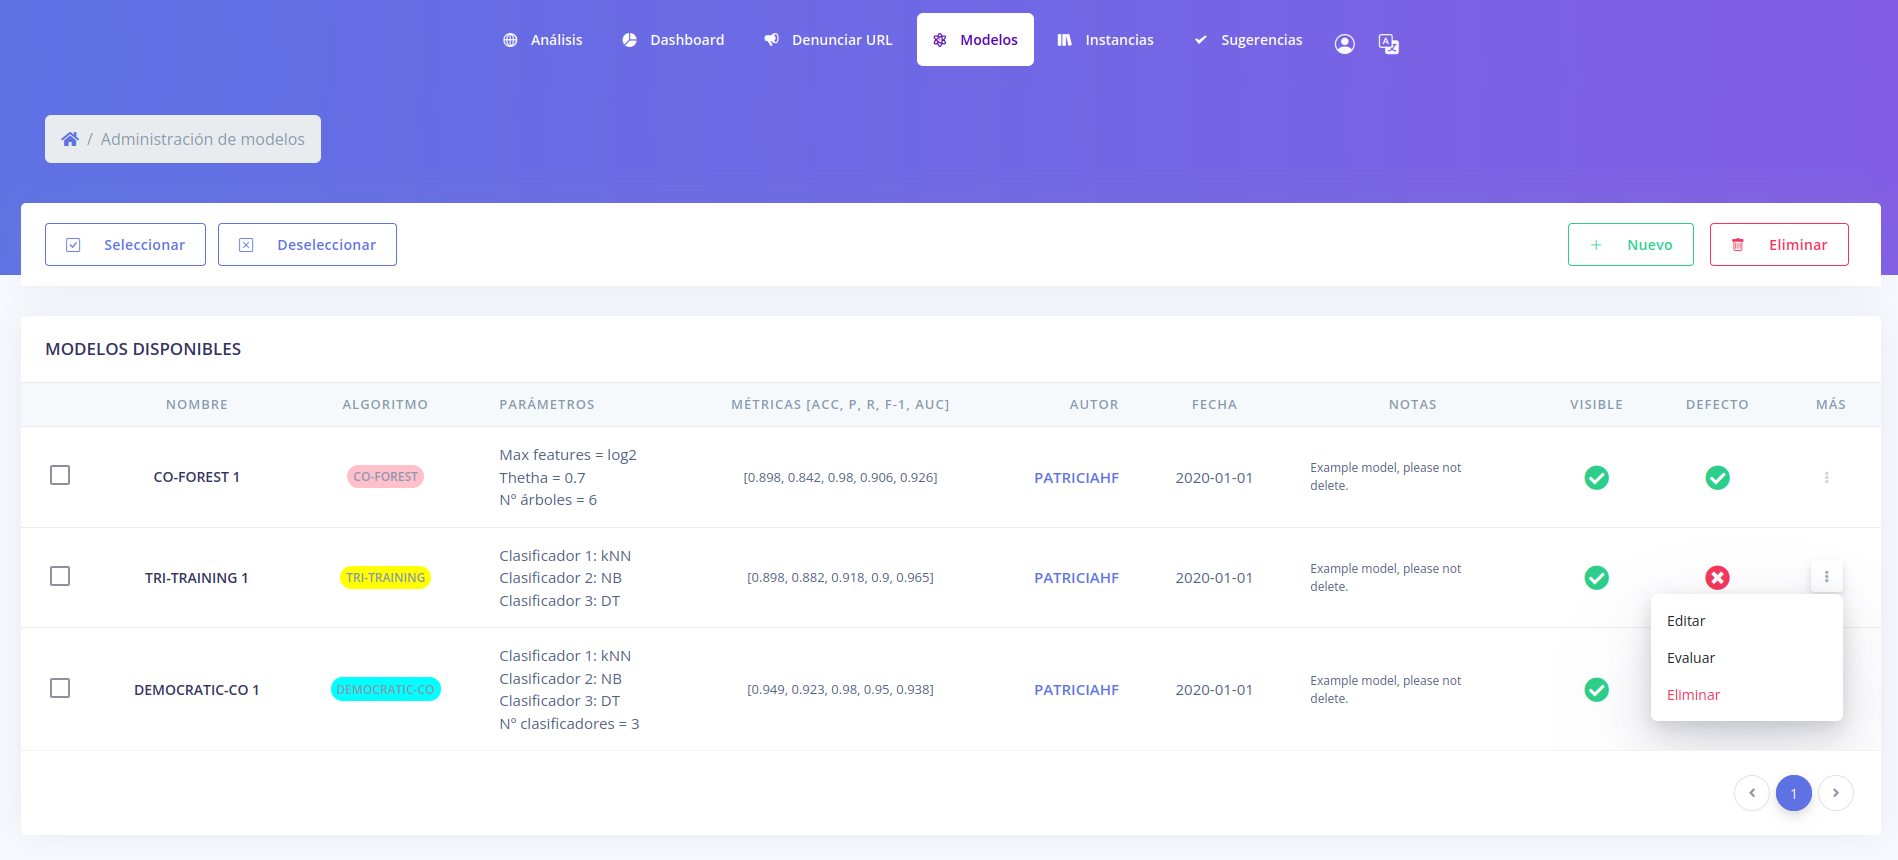
\includegraphics[width=\textwidth]{../img/anexos/user_guide/5_models}
	\label{e-5:models}
\end{figure}

\subsubsection{Nuevo modelo}
\label{s-e:nuevo-modelo}

\begin{figure}[h]
	\caption[Manual de usuario: nuevo modelo]{Formulario de creación de nuevos modelos.}
	\centering
	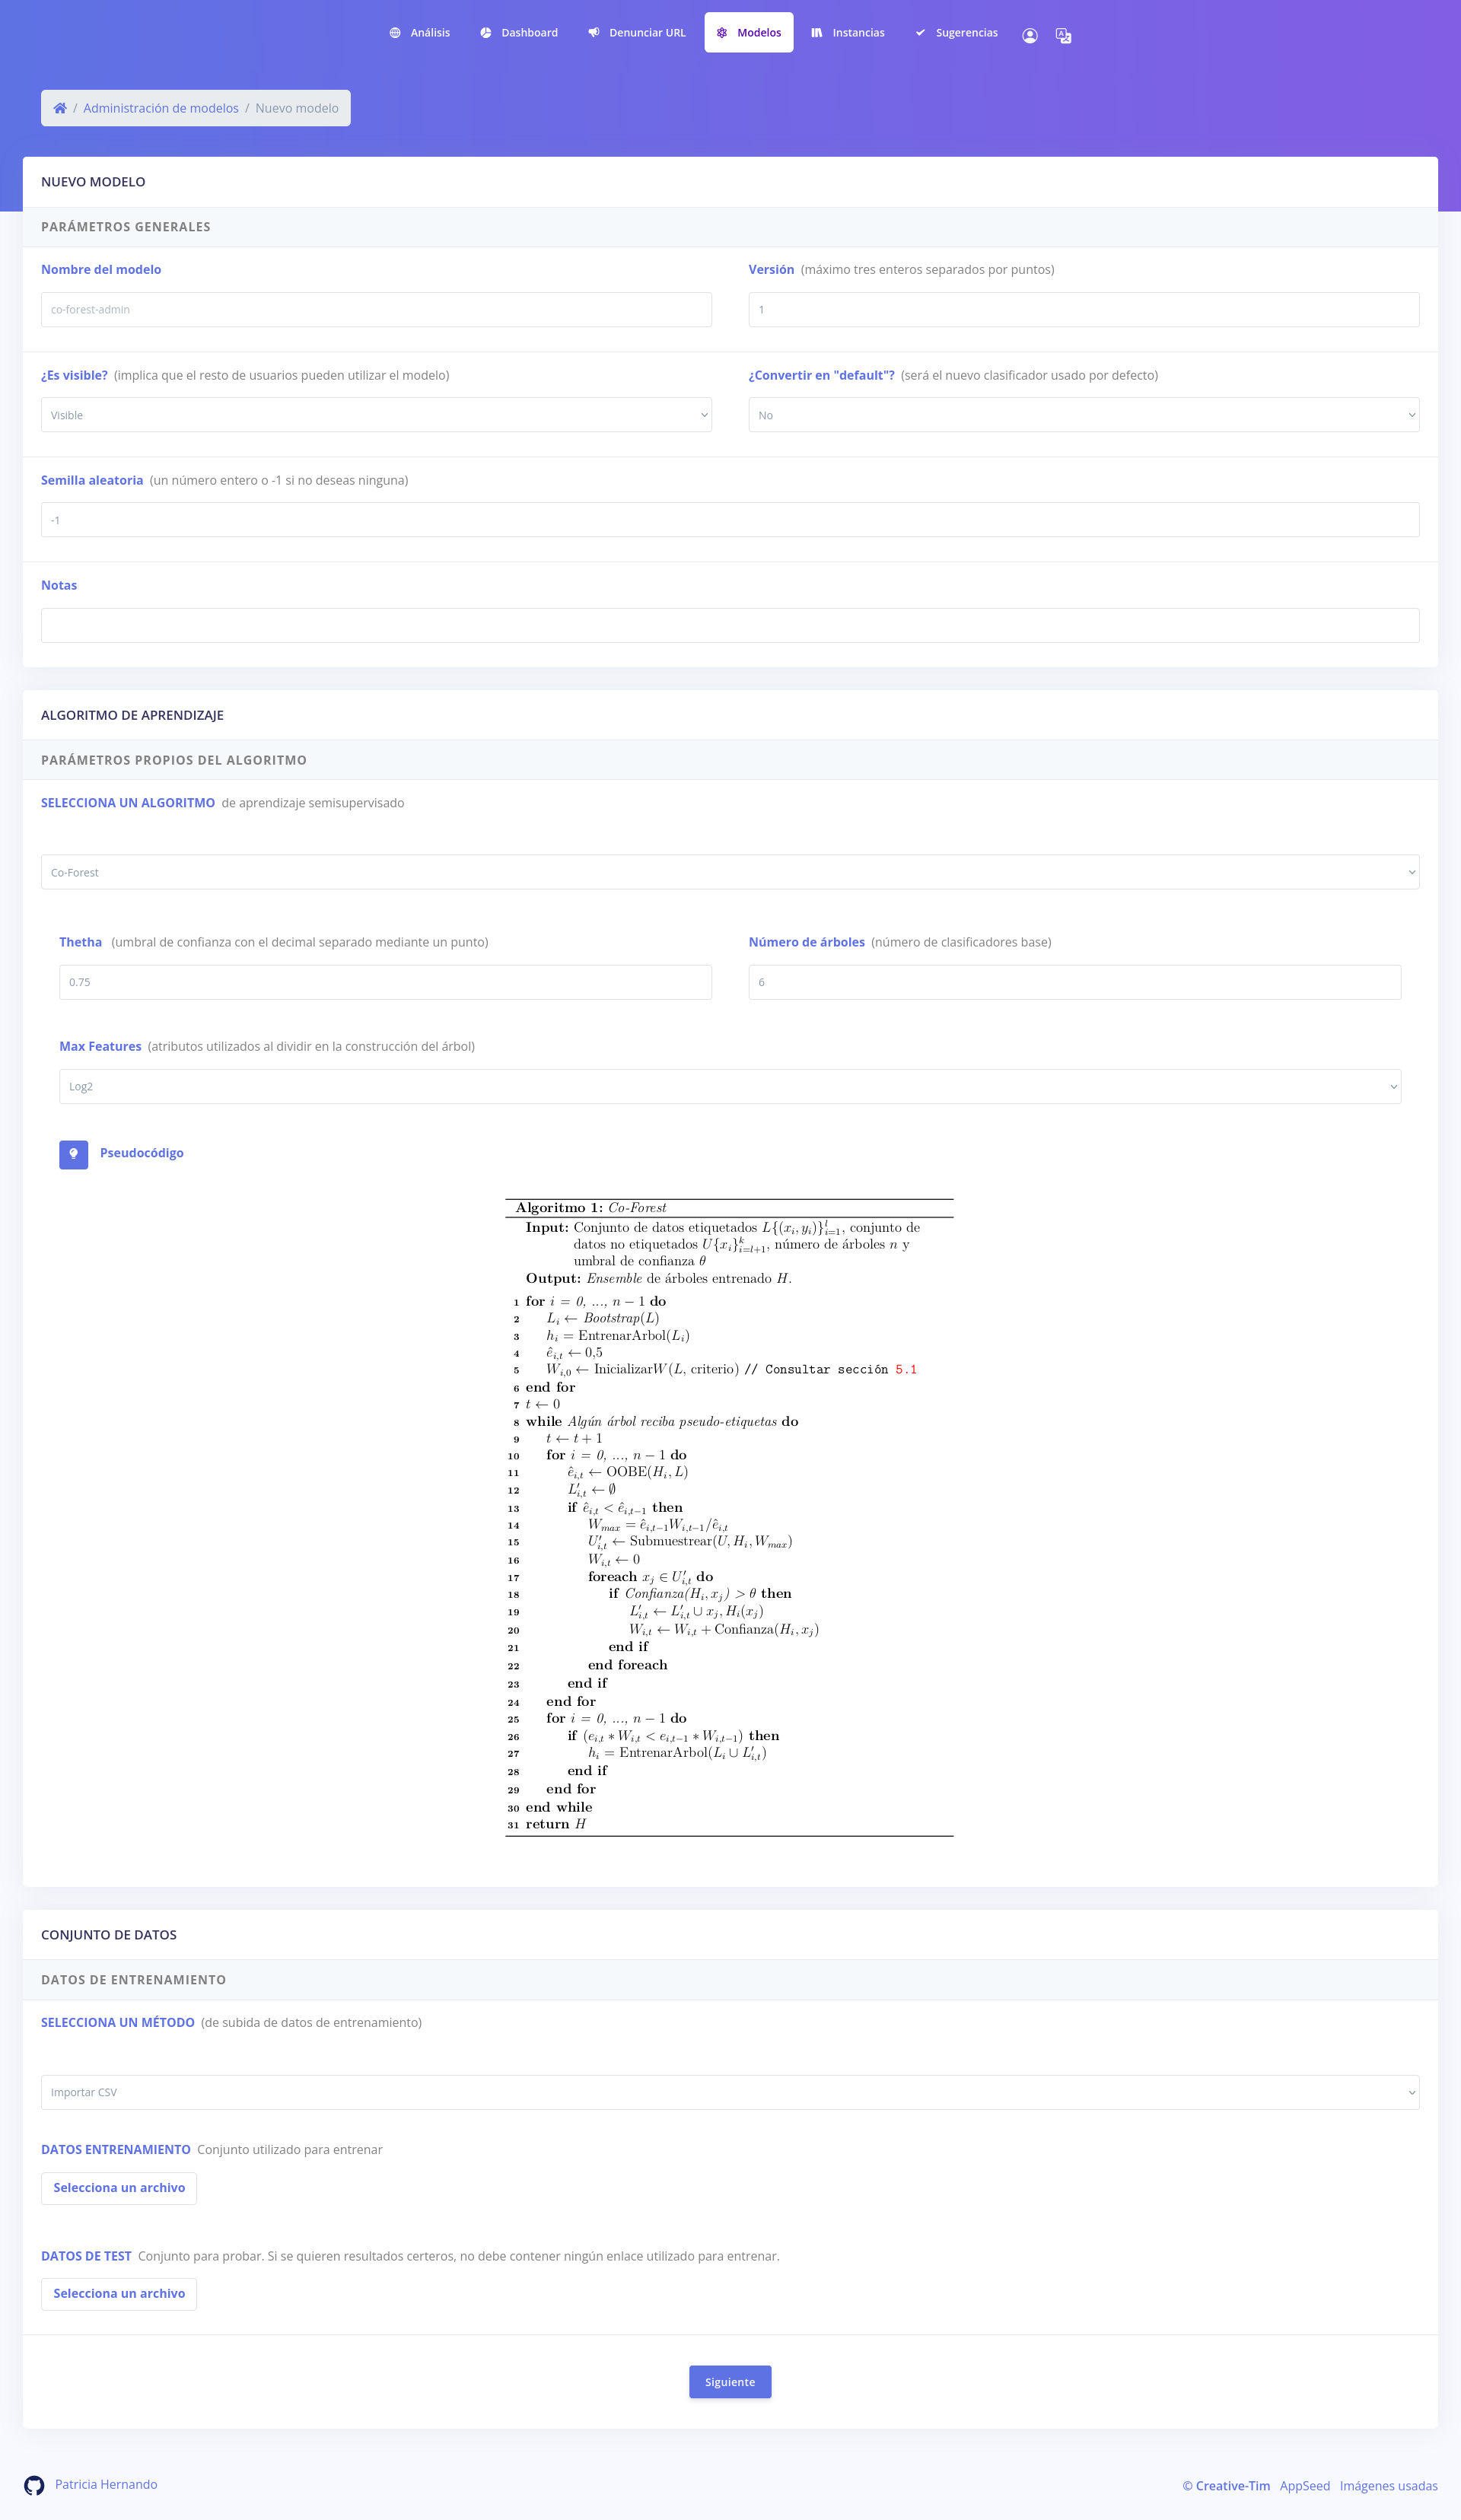
\includegraphics[scale=0.14]{../img/anexos/user_guide/5_new_model}
	\label{e-5:new-model}
\end{figure}

Para crear un modelo, basta con pulsar en el botón <<nuevo>>. Esta acción redirigirá al usuario a un formulario (imagen~\ref{e-5:new-model}) donde podrá personalizar los parámetros de el clasificador semisupervisado que quiera crear, además de seleccionar el algoritmo deseado. Pulsando en el botón <<bombilla>> se desplegará el pseudocódigo de los \textit{ensembles} disponibles.

Posteriormente se podrá elegir los datos de entrenamiento y \textit{test} con los que se quieren crea y evaluar el modelo. Se ofrecen dos opciones:

\begin{enumerate}
	\item \textbf{Subir un fichero \texttt{csv}}: en este caso, deberá tener el formato adecuado\footnote{El formato correcto consiste en 21 columnas por instancia correspondientes al identificador de la URL, los atributos del vector (\texttt{f1-f19}) y la etiqueta. Se recomienda descargar una URL en la sección <<instancias>> (apartado~\ref{s-e:instances}) para asegurar que el formato es correcto.} y no podrá contener valores <<perdidos>> en ninguna instancia. La ventaja principal es que se puede elegir las URLs a utilizar durante las fases de entrenamiento y \textit{test}.
	\item \textbf{Utilizar el \textit{dataset} de la aplicación}: en este caso, los conjuntos se crean aleatoriamente con el contenido de la base de datos. Se puede parametrizar el porcentaje total de las instancias destinadas a los conjuntos de entrenamiento y \textit{test}. Únicamente se tendrán en cuenta aquellas instancias que posean vector de características, etiquetas y hayan sido revisadas por un administrador.
\end{enumerate}

Es destacable que las instancias deben estar vinculadas mediante un identificador con la base de datos de la aplicación para garantizar que se pueda apartar las instancias ya vistas durante el entrenamiento de la evaluación en fases posteriores. Por ello, si se quiere subir un fichero \texttt{csv}, se recomienda que se haya descargado previamente utilizando la sección <<instancias>> (apartado~\ref{s-e:instances} del manual) de la aplicación.

\subsubsection{Editar modelo}

Como se muestra en la imagen~\ref{e-5:edit-model}, se pueden modificar ciertos parámetros de los modelos existentes. Otros atributos ocultos (como el nombre del fichero con el objeto serializado) se actualizarán automáticamente. Para facilitar la edición, se indica en naranja los valores anteriores al usuario.

\begin{figure}[h]
	\caption[Manual de usuario: editar modelo]{Formulario de edición de modelos existentes.}
	\centering
	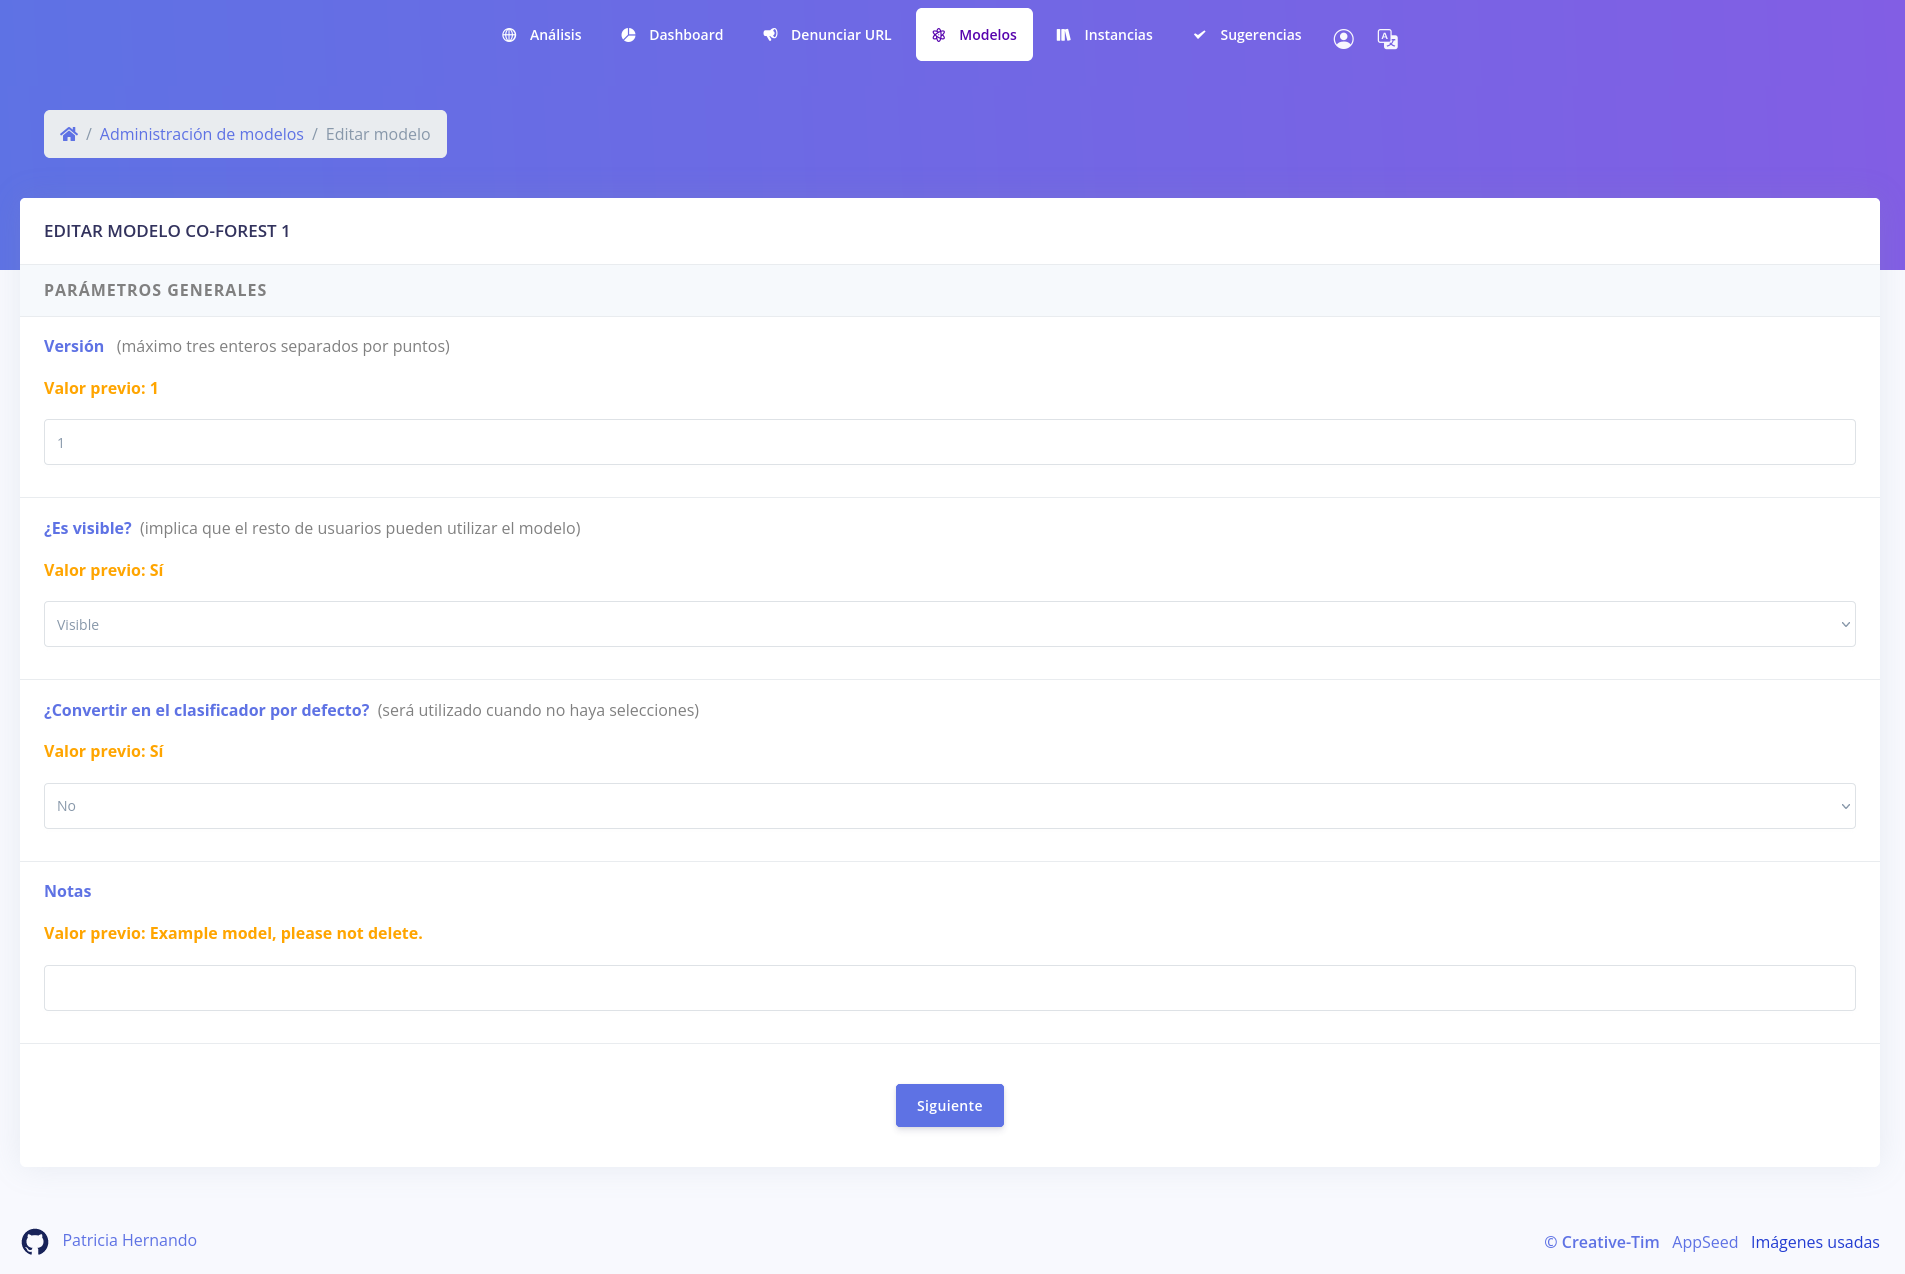
\includegraphics[scale=0.18]{../img/anexos/user_guide/5_edit_model}
	\label{e-5:edit-model}
\end{figure}


\subsubsection{Evaluar modelo}

\begin{figure}[h]
	\caption[Manual de usuario: evaluar modelo]{Página de evaluación de modelos existentes.}
	\centering
	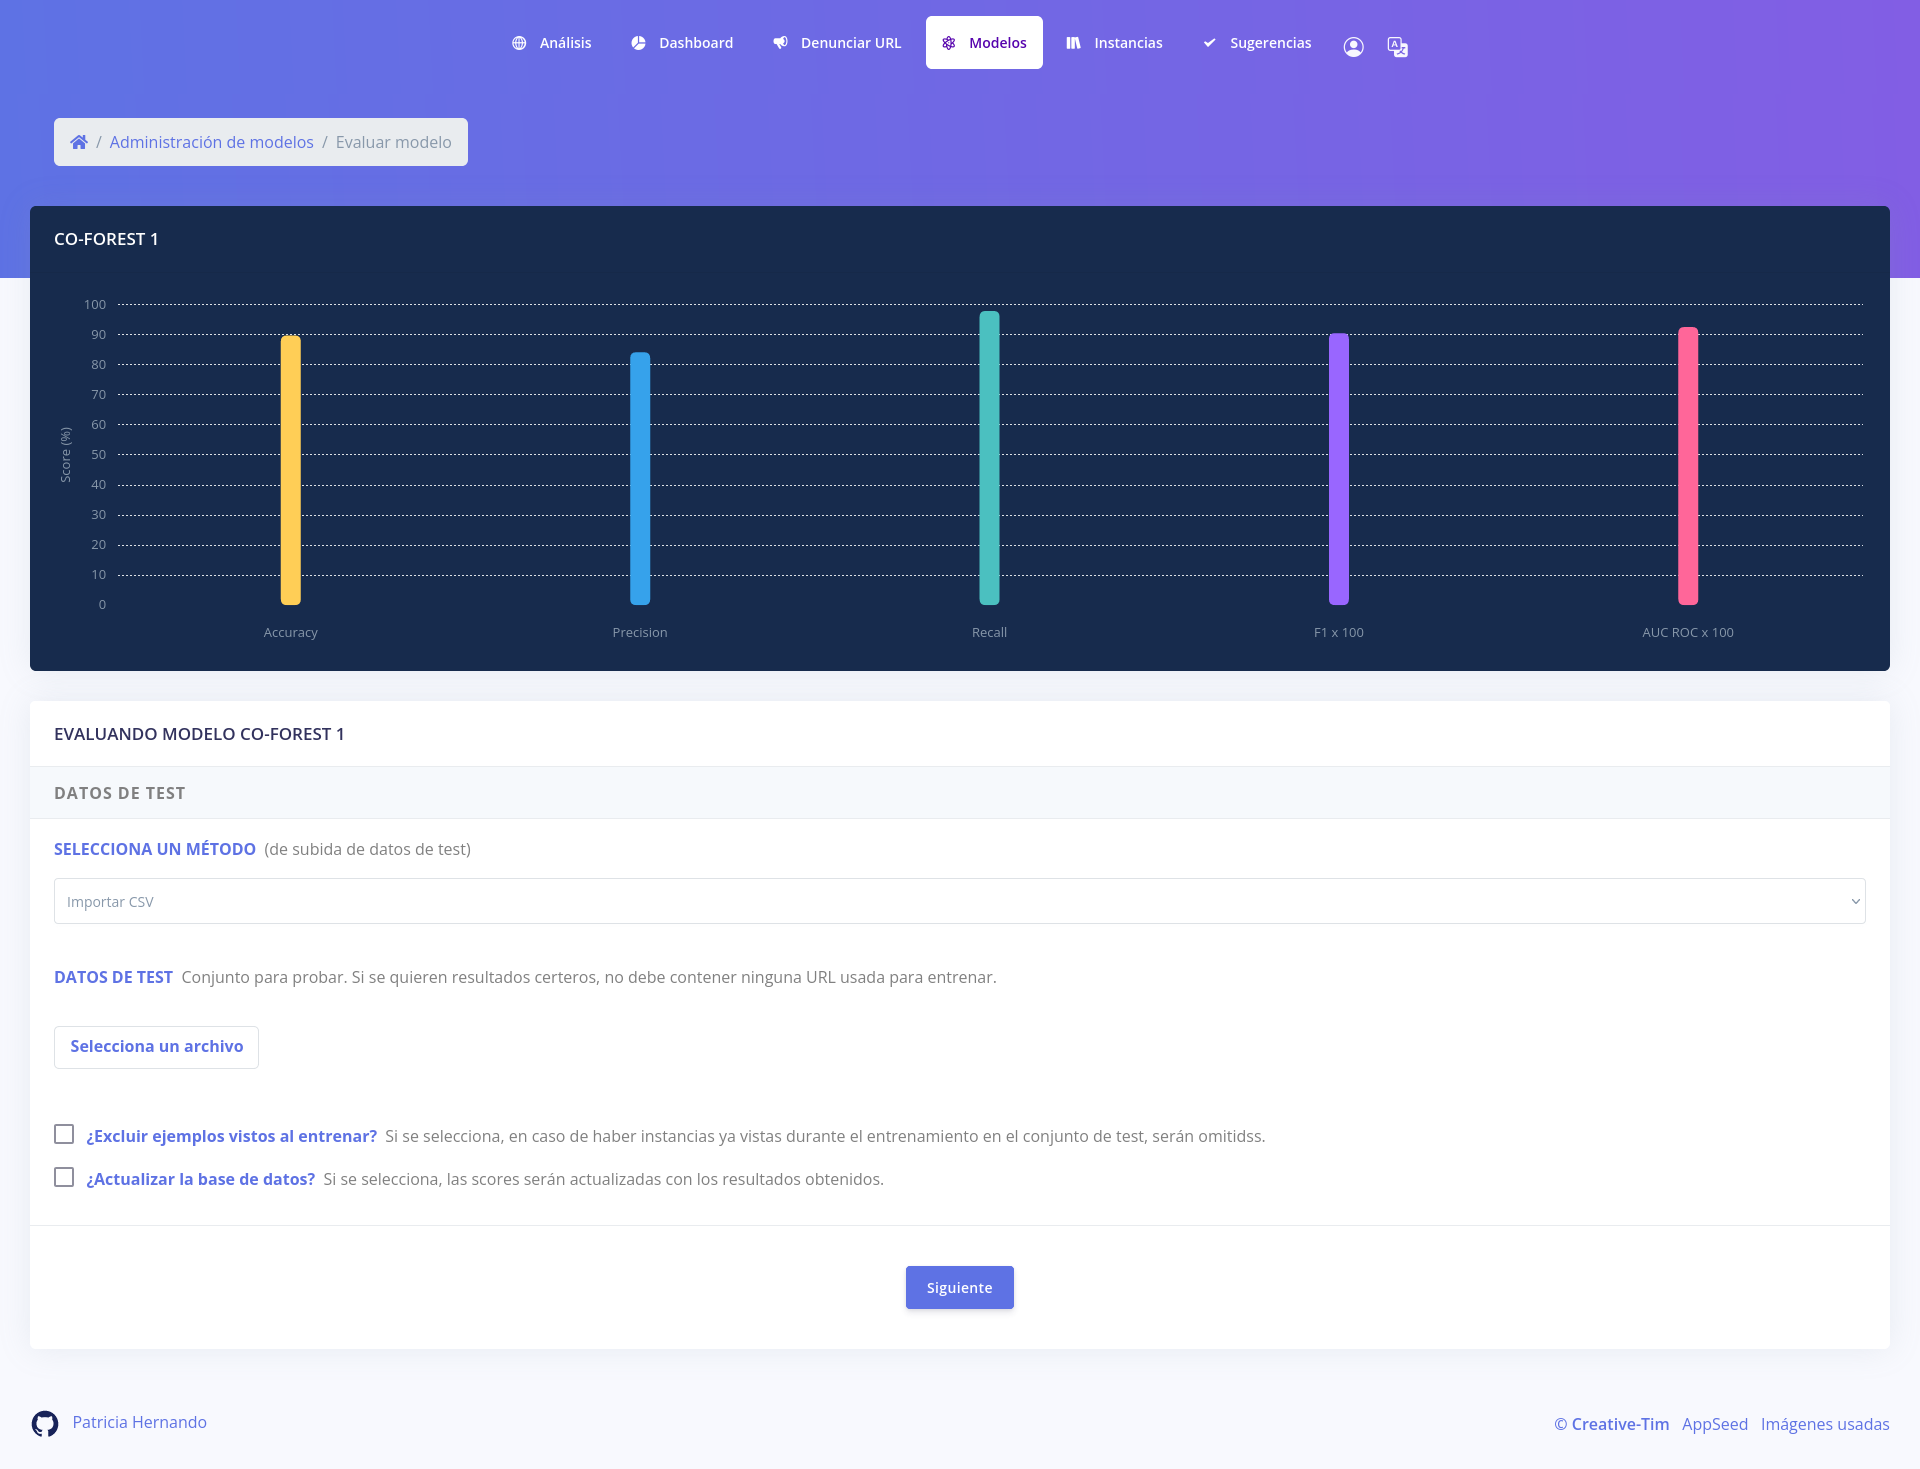
\includegraphics[scale=0.18]{../img/anexos/user_guide/5_test_model}
	\label{e-5:test-model}
\end{figure}


Si se quiere comprobar cómo un modelo reacciona ante nuevas instancias, se puede poner a prueba como se muestra en la imagen~\ref{e-5:test-model}. Para ello, sólo se ha de subir los datos con los que se quiera formar el conjunto de entrenamiento o indicar que se desea utilizar el \textit{dataset} de la aplicación.

Si se quieren actualizar las métricas almacenadas en la base de datos, se puede hacer seleccionando la opción <<actualizar base de datos>>. Se debe tener en cuenta que esto afectará a las gráficas de rendimiento mostradas en el \textit{dashboard}.

Por otro lado, es destacable que si se utilizan instancias vistas durante el entrenamiento para probar un clasificador, es posible que los resultados obtenidos sean optimistas. Por ello, se facilita la opción <<excluir ejemplos vistos durante el entrenamiento>>, de forma que aquellas URLs ya utilizadas serán eliminadas automáticamente de los conjuntos de \textit{test}.

\subsection{Instancias}
\label{s-e:instances}

Los administradores podrán gestionar todas las URLs disponibles en la sección de <<instancias>> (imagen~\ref{e-5:instances}).

\begin{figure}[h]
	\caption[Manual de usuario: página de instancias]{Página de administración de instancias.}
	\centering
	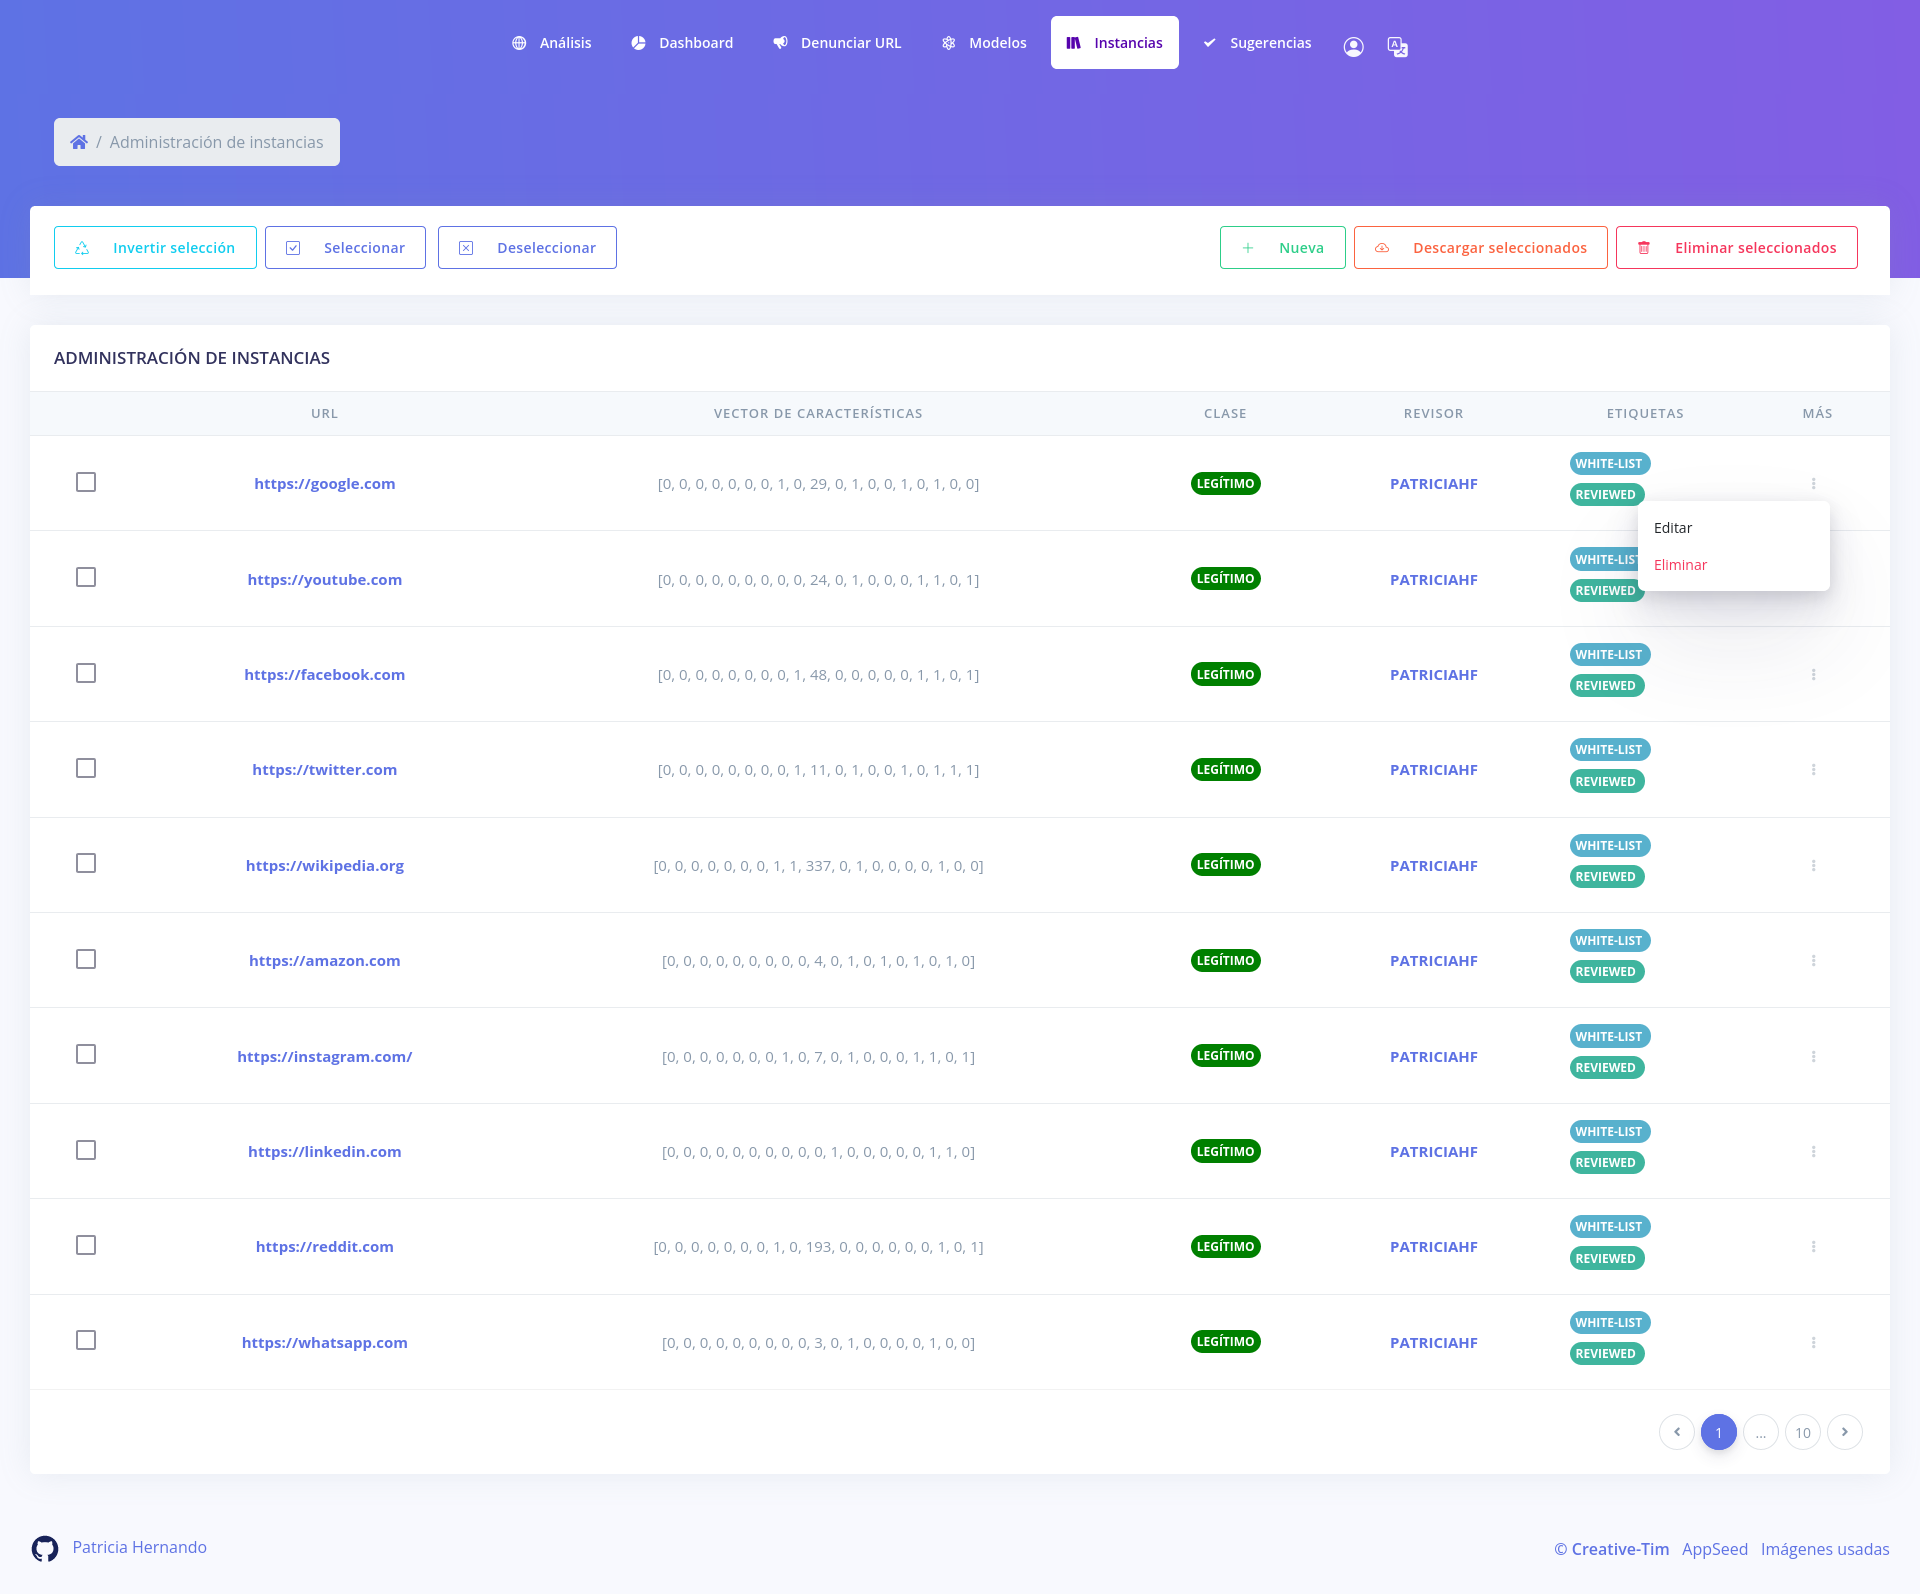
\includegraphics[width=\textwidth]{../img/anexos/user_guide/6_instances}
	\label{e-5:instances}
\end{figure}

\subsubsection{Generar conjuntos de entrenamiento y \textit{test}}

¡Generar conjuntos para entrenar y probar modelos es muy fácil utilizando la aplicación!

Si se selecciona la opción <<utilizar \textit{dataset}>>, (consultar sección~\ref{s-e:nuevo-modelo}), la creación es automática. Sin embargo, la partición se realiza aleatoriamente (con los tamaños indicados).

Si por el contrario se prefiere tener control sobre qué instancias pertenecen a cada conjunto, se recomienda descargar un fichero \texttt{.csv}. Para ello, tan sólo hay que seleccionar las instancias deseadas (se mantienen aunque haya desplazamiento entre páginas) y pulsar el botón de descargar. Se recomienda encarecidamente utilizar el botón <<invertir selección>> para construir el conjunto contrario, ya que pasarán a seleccionarse todas las instancias que antes no lo estaban y viceversa (sin solapamientos).

Se recuerda que aquellas instancias que no contengan vector de características o etiqueta de clase (\textit{phishing} o legítima) no serán descargadas.

\subsubsection{Nueva instancia}

\begin{figure}[h]
	\caption[Manual de usuario: nueva instancia]{Formulario de creación de nuevas instancias.}
	\centering
	\includegraphics[width=\textwidth]{../img/anexos/user_guide/6_new_instance}
	\label{e-5:new-instance}
\end{figure}

\begin{figure}[h]
	\caption[Manual de usuario: etiquetas predeterminadas]{Menú con las etiquetas predeterminadas.}
	\centering
	\includegraphics[scale=0.3]{../img/anexos/user_guide/6_labels}
	\label{e-6:labels}
\end{figure}

Pulsando en el botón de <<nueva>>, se mostrará un formulario que se facilita en la ilustración~\ref{e-5:new-instance}. Para crear una instancia, simplemente hay que rellenarlo. Hay algunas etiquetas predeterminadas que poseen colores propios (se muestran en la imagen~\ref{e-6:labels}). Sin embargo, los administradores pueden añadir las etiquetas que deseen escribiendo el nombre correspondiente y pulsando <<enter>>.

Es relevante destacar que no es necesario que la URL sea llamable para crear la instancia. Esta decisión se ha tomado debido a que muchas páginas de \textit{phishing} dejan de estar disponibles a los pocos días de su creación y, además, sólo los administradores pueden crear entradas (se entiende que son miembros de la organización y no van a introducir <<basura>>). Sin embargo, es destacable que una URL debe estar disponible para poder generar su vector de características y así poder ser utilizada para entrenar y evaluar modelos.

En cualquiera de los casos, se entiende que generar un vector es un proceso lento. Por ello, se puede posponer para más adelante (opción de <<editar instancias>>).

\subsubsection{Editar instancia}

\begin{figure}[h]
	\caption[Manual de usuario: editar instancia]{Formulario de edición de instancias existentes.}
	\centering
	\includegraphics[scale=0.18]{../img/anexos/user_guide/6_edit_instance}
	\label{e-5:edit-instance}
\end{figure}

Todas las instancias existentes pueden ser editadas a través del formulario que se muestra en la imagen~\ref{e-5:edit-instance}. Nuevamente, se muestran los valores anteriores en naranja para facilitar el proceso. Desde este menú, se puede elegir si regenerar el vector de características.

Es destacable que, en caso de conflicto de etiquetas (ejemplo: se selecciona pertenencia a una lista negra y se pone como etiqueta \texttt{white-list}), las menos prioritarias serán eliminadas.


\subsection{Sugerencias}
\label{s-e:sugerencias}

Cuando un usuario registrado reporta un análisis que considera erróneo (consultar sección~\ref{s-e:report-false-analy}) o denuncia una URL por pertenecer a una lista blanca o negra (consultar sección~\ref{s-e:report-url}), se crea una nueva entrada en la sección de <<sugerencias>>. También se crean nuevas sugerencias cuando un usuario registrado analiza una URL (para recordar al administrador que revise la nueva instancia).

\begin{figure}[h]
	\caption[Manual de usuario: administrar sugerencias]{Página de administración de sugerencias o \textit{reports}.}
	\centering
	\includegraphics[width=\textwidth]{../img/anexos/user_guide/7_reports}
	\label{e-7:reports}
\end{figure}

Cada sugerencia realizada contiene una etiqueta en función del tipo, y se pueden aceptar o descartar pulsando en <<más>> (como se muestra en la imagen~\ref{e-7:reports}).

Aceptar una sugerencia implica que se modifica la URL afectada. Es decir, si se acepta una sugerencia que indica \texttt{suggestion-white-list}, la instancia pasará a ser marcada como perteneciente a una lista blanca. Si se acepta una sugerencia cuya etiqueta es~\texttt{suggestion-phishing}, la URL afectada se clasificará como \textit{phishing}, aunque fuese legítima anteriormente. Todas las etiquetas que presenten conflicto con el nuevo estado serán eliminadas.

\subsection{Usuarios, perfil, inicio de sesión y registro}

Cualquier usuario visitante podrá crear una cuenta (imagen~\ref{e-8:register}) e iniciar sesión en la \textit{web} (imagen~\ref{e-8:login}) proporcionando las credenciales que considere. Sin embargo, únicamente los administradores tendrán acceso a la funcionalidad completa de la aplicación\footnote{Para saber qué usuario puede realizar cada acción, consultar el diagrama de casos de uso~\ref{b:diagrama-cu}.}.

\begin{figure}[h]
	\caption[Manual de usuario: crear nueva cuenta]{Página de creación de nuevas cuentas.}
	\centering
	\includegraphics[scale=0.25]{../img/anexos/user_guide/8_register}
	\label{e-8:register}
\end{figure}

\begin{figure}[h]
	\caption[Manual de usuario: inicio de sesión]{Página de inicio de sesión.}
	\centering
	\includegraphics[width=\textwidth]{../img/anexos/user_guide/8_login}
	\label{e-8:login}
\end{figure}

Los usuarios registrados podrán, además, visualizar su perfil pulsando en el icono de usuario de la barra de navegación (consultar imagen~\ref{e-9:navbar}) y posteriormente en <<perfil>>. Esto renderizará la información correspondiente como se representa en la imagen~\ref{e-8:profile}, además de ciertas estadísticas como el número de URLs que el usuario ha denunciado que han sido aceptadas y el número de URLs que se encuentran en revisión.

\begin{figure}[h]
	\caption[Manual de usuario: perfil]{Perfil de un usuario que ha iniciado sesión en la aplicación.}
	\centering
	\includegraphics[width=\textwidth]{../img/anexos/user_guide/8_profile}
	\label{e-8:profile}
\end{figure}

Según los permisos que tenga el usuario, la barra de navegación mostrará unas funcionalidades u otras. El menú más sencillo corresponde a los usuarios visitantes y se muestra (con el menú de internacionalización desplegado) en la imagen~\ref{e-9:navbar-2}, mientras que la barra más compleja pertenece a los administradores y se muestra en la imagen~\ref{e-9:navbar} (con el menú de usuario desplegado).
\begin{figure}[h]
	\caption[Manual de usuario: barra navegación (usuario iniciado)]{Barra de navegación correspondiente a un administrador}
	\centering
	\includegraphics[width=\textwidth]{../img/anexos/user_guide/9_navbar_init}
	\label{e-9:navbar}
\end{figure}

\begin{figure}[h]
	\caption[Manual de usuario: barra navegación (visitante)]{Barra de navegación correspondiente a un usuario visitante.}
	\centering
	\includegraphics[width=\textwidth]{../img/anexos/user_guide/9_navbar_no_init}
	\label{e-9:navbar-2}
\end{figure}


\subsection{Internacionalización}

Para cambiar el idioma de la aplicación, tan sólo se ha de pulsar en el icono correspondiente a idiomas en la barra de navegación. Esto abrirá un menú desplegable donde se podrá seleccionar el idioma deseado (consultar imagen~\ref{e-9:navbar-2}). Esta opción está disponible tanto para usuarios registrados como para visitantes.


\subsection{Pantallas de error}

Todos los errores que ocurran internamente son tratados para evitar que afecte a la experiencia del usuario. En caso de tratarse de excepciones, se mostrarán mensajes informativos adecuados. Por otro lado, los errores más graves tienen asociadas pantallas concretas (por supuesto, internacionalizadas) en función del tipo de código de error. Algunos ejemplos se muestran en las imágenes \ref{e-0:error-403}, \ref{e-0:error-404}, \ref{e-0:error-408} y~\ref{e-0:error-500}.

\begin{figure}[h]
	\caption[Manual de usuario: error 403]{Página de error 403.}
	\centering
	\includegraphics[scale=0.27]{../img/anexos/user_guide/0_error_403}
	\label{e-0:error-403}
\end{figure}

\begin{figure}[h]
	\caption[Manual de usuario: error 404]{Página de error 404.}
	\centering
	\includegraphics[scale=0.27]{../img/anexos/user_guide/0_error_404}
	\label{e-0:error-404}
\end{figure}

\begin{figure}[h]
	\caption[Manual de usuario: error 408]{Página de error 408. Correspondiente a los \textit{timeouts} de Heroku.}
	\centering
	\includegraphics[scale=0.27]{../img/anexos/user_guide/0_error_408}
	\label{e-0:error-408}
\end{figure}

\begin{figure}[h]
	\caption[Manual de usuario: error 500]{Página de error 500.}
	\centering
	\includegraphics[scale=0.27]{../img/anexos/user_guide/0_error_500}
	\label{e-0:error-500}
\end{figure}


\subsection{Responsividad y dispositivos móviles}

La página \textit{web} diseñada está adaptada para ser ejecutada en dispositivos móviles y para adaptarse a las medidas de las pantallas más pequeñas. Un ejemplo de como se visualiza el \textit{dashboard} en un dispositivo móvil se muestra en la imagen~\ref{e-0:dashboard-mobile}. La navegación, en este caso, se convierte en un menú <<hamburguesa>> (imagen~\ref{e-0:menu-mobile}).

\begin{figure}[h]
	\caption[Manual de usuario: \textit{dashboard} (versión móvil)]{\textit{Dashboard} visualizado desde el navegador de un teléfono.}
	\centering
	\includegraphics[scale=0.1]{../img/anexos/user_guide/0_dashboard_mobile}
	\label{e-0:dashboard-mobile}
\end{figure}

\begin{figure}[h]
	\caption[Manual de usuario: menú (versión móvil)]{Menú de navegación visualizado desde un dispositivo móvil.}
	\centering
	\includegraphics[scale=0.1]{../img/anexos/user_guide/0_menu_mobile}
	\label{e-0:menu-mobile}
\end{figure}


\bibliographystyle{plain}
\bibliography{bibliografiaAnexos}

\clearpage
\thispagestyle{empty}
\newenvironment{bottompar}{\par\vspace*{\fill}}{\clearpage}
\begin{bottompar}
\begin{figure*}[b]
	\centering
	\includegraphics[scale=0.3]{../img/cc}
\end{figure*}
\end{bottompar}
\end{document}
